\chapter{The Large Hadron Collider}
\label{lhc_overview}

\begin{figure}[h]
   \centering
  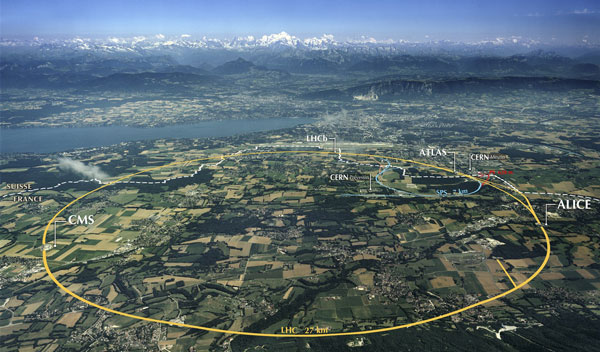
\includegraphics[width=1.0\textwidth]{Figures/LHC_Diagrams/LHC_Aerial_View.jpg}
  \caption{Aerial view of the LHC complex, spanning the French-Swiss border~\cite{LHC:Aerial_View}} \label{fig:lhc_aerial_with_labels}
\end{figure}

\par The \acrfull{lhc}, is a superconducting, proton-proton,
accelerator and collider operated by the \acrfull{cern} laboratory in
Geneva, Switzerland~\cite{lhc:machine_description}.  Figure
\ref{fig:lhc_aerial_with_labels} shows an aerial view of the LHC
complex, with the main laboratory campus being labeled as CERN, with
four of the detector experiments being labeled as ALICE, ATLAS, CMS,
and LHCb.  Three smaller experiments, not pictured, also use the LHC
ring, and are TOTEM, LHCf, and MOeDAL.  It was designed to elucidate
the mechanism of electroweak symmetry breaking and explore \TeV scale
of particle physics.  As such, it is required to produce a large
number of high center-of-mass energy events.  The high center-of-mass
energy allows the creation of heavy particles, while a large
luminosity allows for the creation of rare processes.  The number of events
produced at a collider is a product of the luminosity of the collider
and the total cross-section for the objects being collided.  

\begin{equation}\label{eq:Nevents}
N_{events} = L\sigma_{event}
\end{equation}

\noindent  The cross-section, $\sigma_{event}$, can be estimated from the
theory of the Standard Model as described in section
\ref{qft_overview} and validated by measurement at detectors, such as
CMS, as shown in section \ref{ttH_backgrounds_overview}.  The
luminosity is a control of the experiment, and for Gaussian
distributed beams, is given by the equation:

\begin{equation}\label{eq:lumi}
L = \frac{ N_{b}^{2}n_{b}f_{rev}\gamma_{r}
}{ 4\pi\epsilon_{n}\beta^{\ast} }F
\end{equation}

\noindent The parameters of this equation and their value for the LHC
is as follows:
\begin{itemize}
\item $N_{b}$ - Number of of particles per bunch, squared since there
  are two beams.  The mechanism of achieving such high energies is
  based in Radio-Frequency (RF) cavity technology, which clusters the
  protons together into packets, which are all accelerated and
  collided together.  For the LHC, $N_{b} = 1.15 \times 10^{11}$.
\item $n_{b}$ - Number of bunches per beam.  The maximum design for
  the LHC allows for $n_{b} = 2808$ bunches, however in practice,
  lower number of bunches have been run with in order to create more
  time between bunch crossings.  
\item $f_{rev}$ - Revolution frequency of the protons in the LHC
  ring.  This is determined by ring circumference, and for the LHC,
  $f_{rev} = 11.2$ kHz. 
\item $\gamma_{r}$ - This is the relativistic gamma-factor, determined
  by the speed, and thus the center of mass energy of the collisions.  
\item $\epsilon_{n}$ - This is the normalized transverse emmitance of
  the beam, which describes the RMS spread of the beam in its
  transverse plane.  For the LHC $\epsilon_{n} = 3.75~\mu$m.  
\item $\beta^{\ast}$ - Is the minimum of the $\beta$ function, which
  is defined as the square of the transverse beam-size divided by
  $\epsilon_{n}$.  It is minimized at interaction regions, where the
  beams are being squeezed into the smallest region possible, to
  maximize the probability of protons colliding during each bunch
  crossing.  For the LHC, $\beta^{\ast} = 0.55$ 
\item $F$ - This is the efficiency for having the two beams head-on,
  and is determined by the crossing angle at which the two
  counter-rotating beams meet each other.  
\end{itemize}

\noindent The LHC is designed to deliver a maximum luminosity of L =
10$^{34}$cm$^{-2}$s$^{-1}$ to the CMS and ATLAS experiments, with a
maximum center-of-mass energy of $\sqrt{s}=14\TeV$.  


\begin{figure}[h]
   \centering
  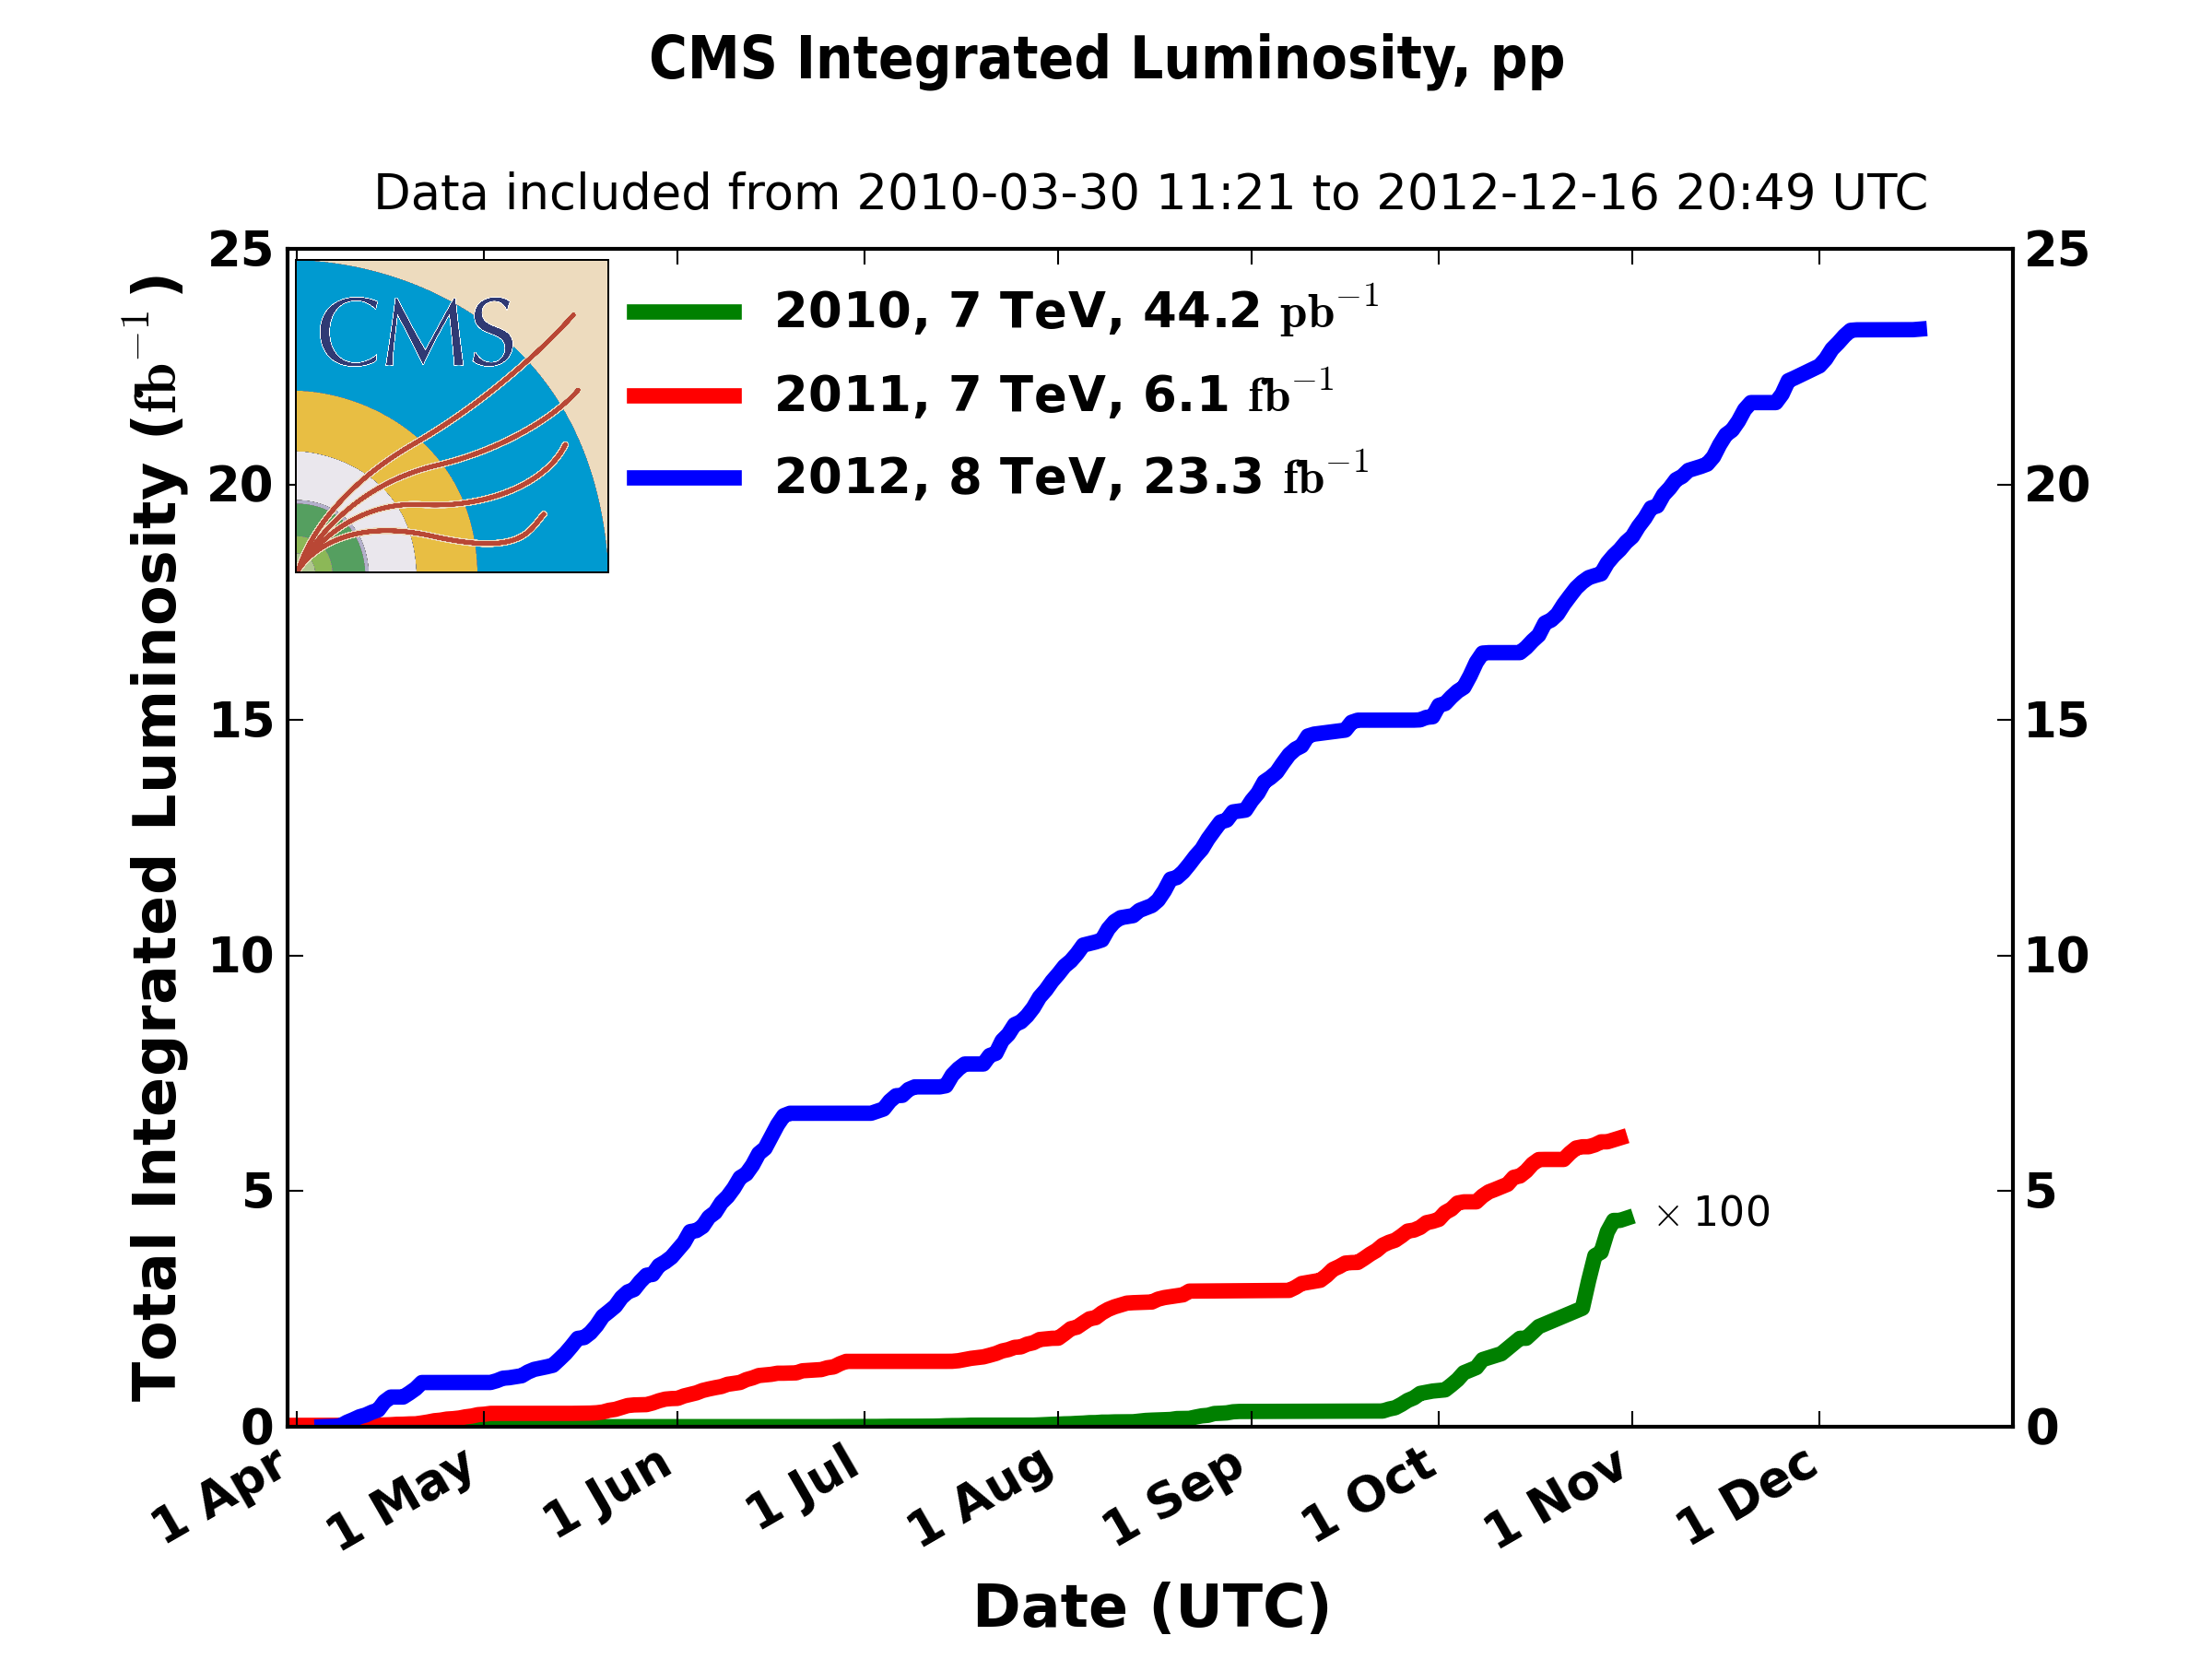
\includegraphics[width=0.8\textwidth]{Figures/Experimental_Results/CMS__int_lumi_cumulative_pp_2.png}
  \caption{Integrated Luminosity delivered to the CMS experiment from
    2010-12 \cite{LHC:Lumi_delivered}} \label{fig:cms_integrated_lumi}
\end{figure}

\par In 2010-11, the LHC ran at center-of-mass energy,
$\sqrt{s}=7\TeV$ and delivered $\sim6\fbinv$ of data to the CMS
experiment.  In 2012, it ran at $\sqrt{s}=8\TeV$ and collected
$\sim23\fbinv$.  Figure \ref{fig:cms_integrated_lumi} shows a diagram of
the luminosity collected as a function of time for each year running.  

\par The next sections will describe the LHC accelerator complex, the
chain of events leading up to collisions of protons at the LHC, and
the associated technologies that allow for the control and operation
of the high-energy, high-luminosity beams that allow the CMS and ATLAS
experiments to search for heavy particles and rare-processes.  


\section{The LHC Accelerator Complex}
\label{lhc_injection_chain}

\par The main LHC ring is a 26.7 km tunnel, that is 45 m to 170 m
underneath the surface of the earth, with 1.4$\%$ slope towards Lake
Leman.  It extends across the French-Swiss border, into the French
countryside.  The tunnel was originally constructed between 1984 and 1989 for
the Large Electron Positron (LEP) experiment that is famous for it's
precision measurements of several Standard Model
parameters~\cite{lhc:machine_description}.  The choice to build the
ring underground was driven by real estate costs, but the underground
setting also provides natural radiation shielding from the beam-line
and greatly reduces the impact of cosmic radiation on the detectors.  

\begin{figure}[h]
   \centering
  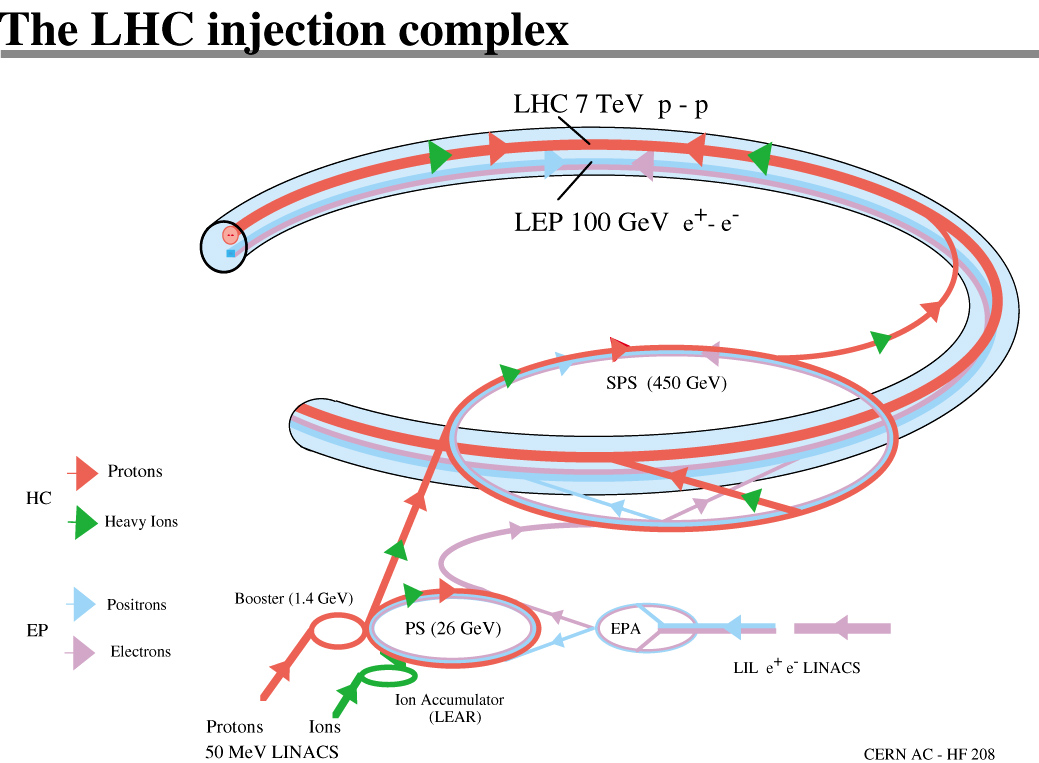
\includegraphics[width=0.8\textwidth]{Figures/LHC_Diagrams/LHC_injection_complex.jpg}
  \caption{The LHC accelerator complex, taking protons from a bottle
    of Hydrogen at the Linac2, all the way to the LHC
    ring \cite{Jean-Luc:841568}} \label{fig:lhc_accelerator_complex}
\end{figure}

\par The LHC also utilizes the existing accelerator complex from the
LEP experiment, which is shown in figure
\ref{fig:lhc_accelerator_complex}.  The complex is composed a series
of increasingly powerful accelerators that gradually increase the
energy of the protons.  

\begin{figure}{h}
    \centering
    \begin{subfigure}[h]{0.4\textwidth}
        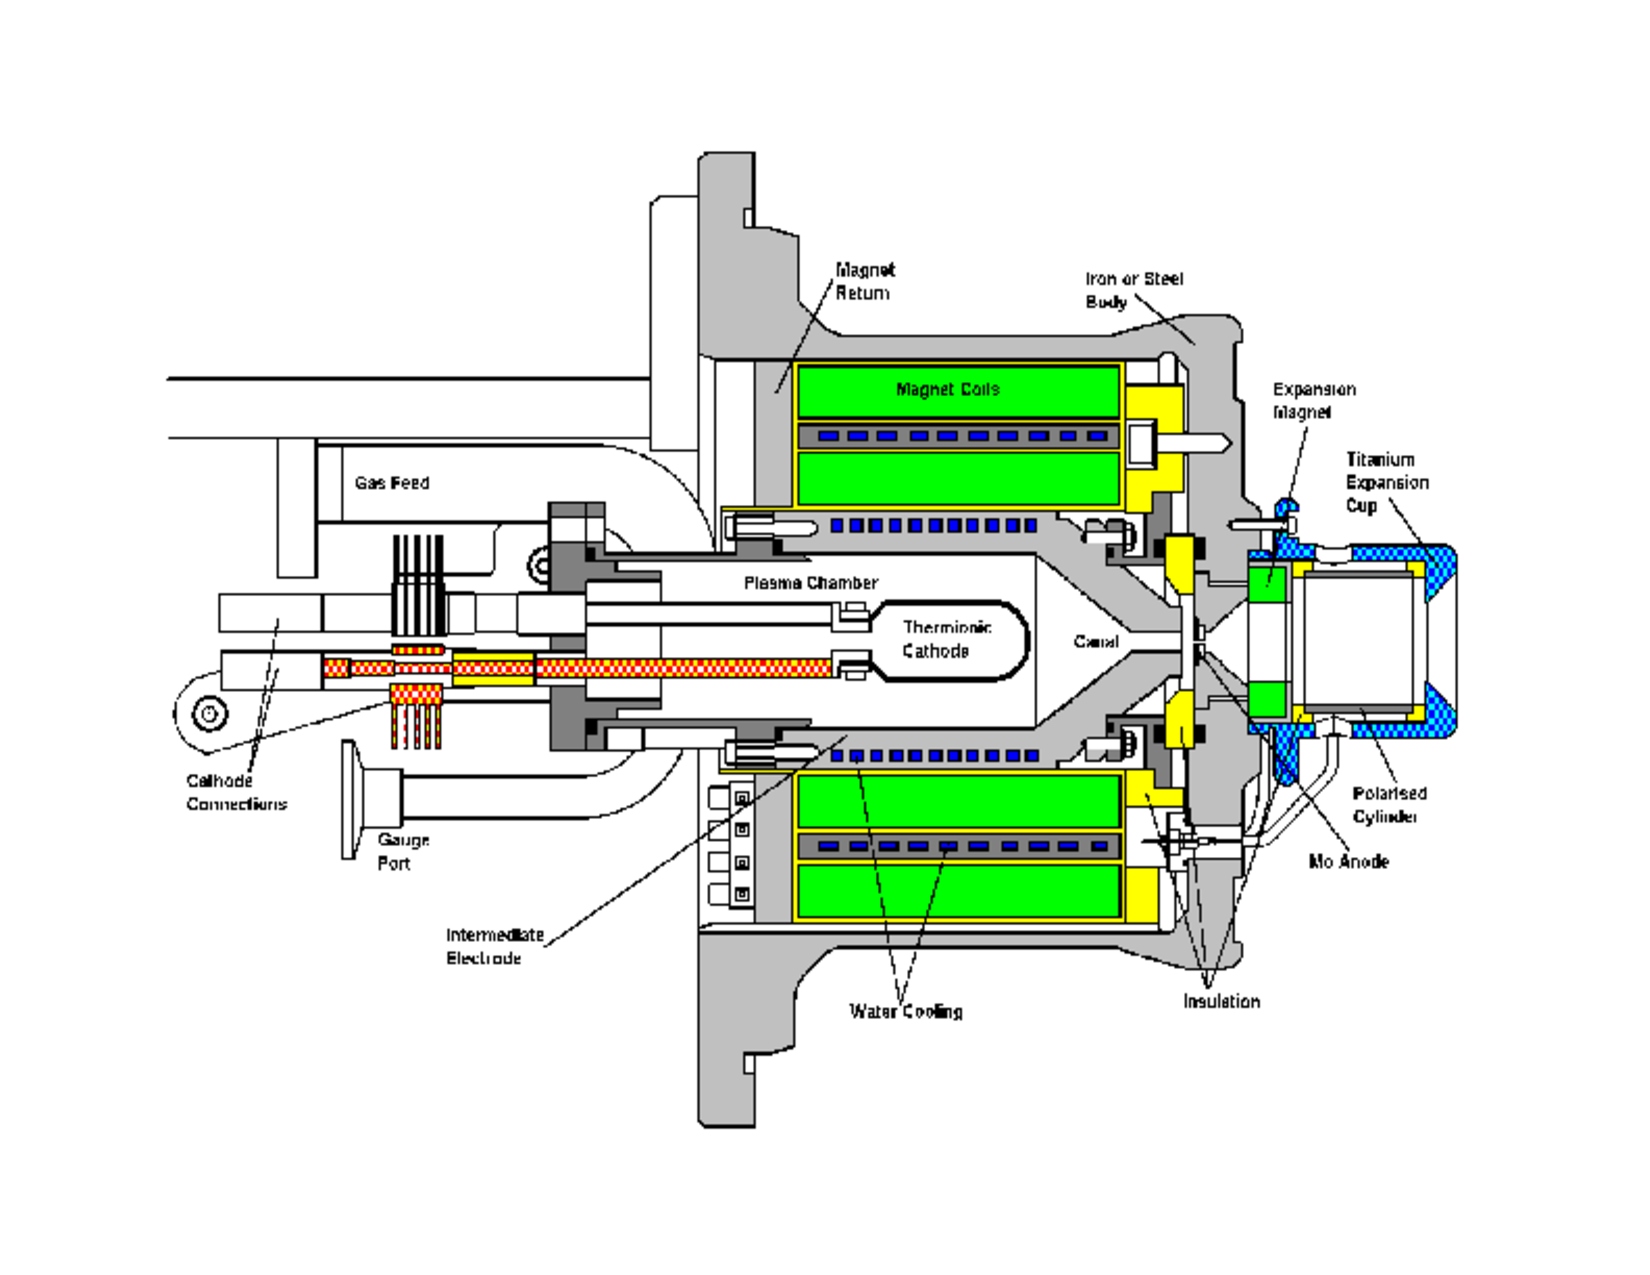
\includegraphics[width=\textwidth]{Figures/LHC_Diagrams/LHC__Linac2__Duoplasmatron_Schematic.pdf}
        \caption{Schematic of the duoplasmatron ion source, which
          creates a proton beam from source bottle of Hydrogen \cite{LHC:LHC_linac2_duoplasmatron_schematic}}\label{fig:duoplasmatron_schematic}
      \end{subfigure}
      ~ %add desired spacing between images, e. g. ~, \quad, \qquad, \hfill etc.
      % (or a blank line to force the subfigure onto a new line)
      \begin{subfigure}[h]{0.4\textwidth}
        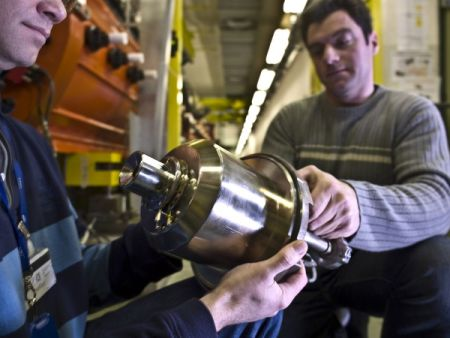
\includegraphics[width=\textwidth]{Figures/LHC_Diagrams/LHC__Linac2__Duoplasmatron__CF002521-ProtonSourceDuoplasmatronRichardChristianss.jpg}
        \caption{The Duoplasmatron used in the Linac2 at CERN, the
          source of the LHC proton beam \cite{LHC:LHC_linac2_duoplasmatron_image}}\label{fig:duoplasmatron_actual}
      \end{subfigure}
       ~ %add desired spacing between images, e. g. ~, \quad, \qquad, \hfill etc.
      % (or a blank line to force the subfigure onto a new line)
      \begin{subfigure}[h]{0.4\textwidth}
        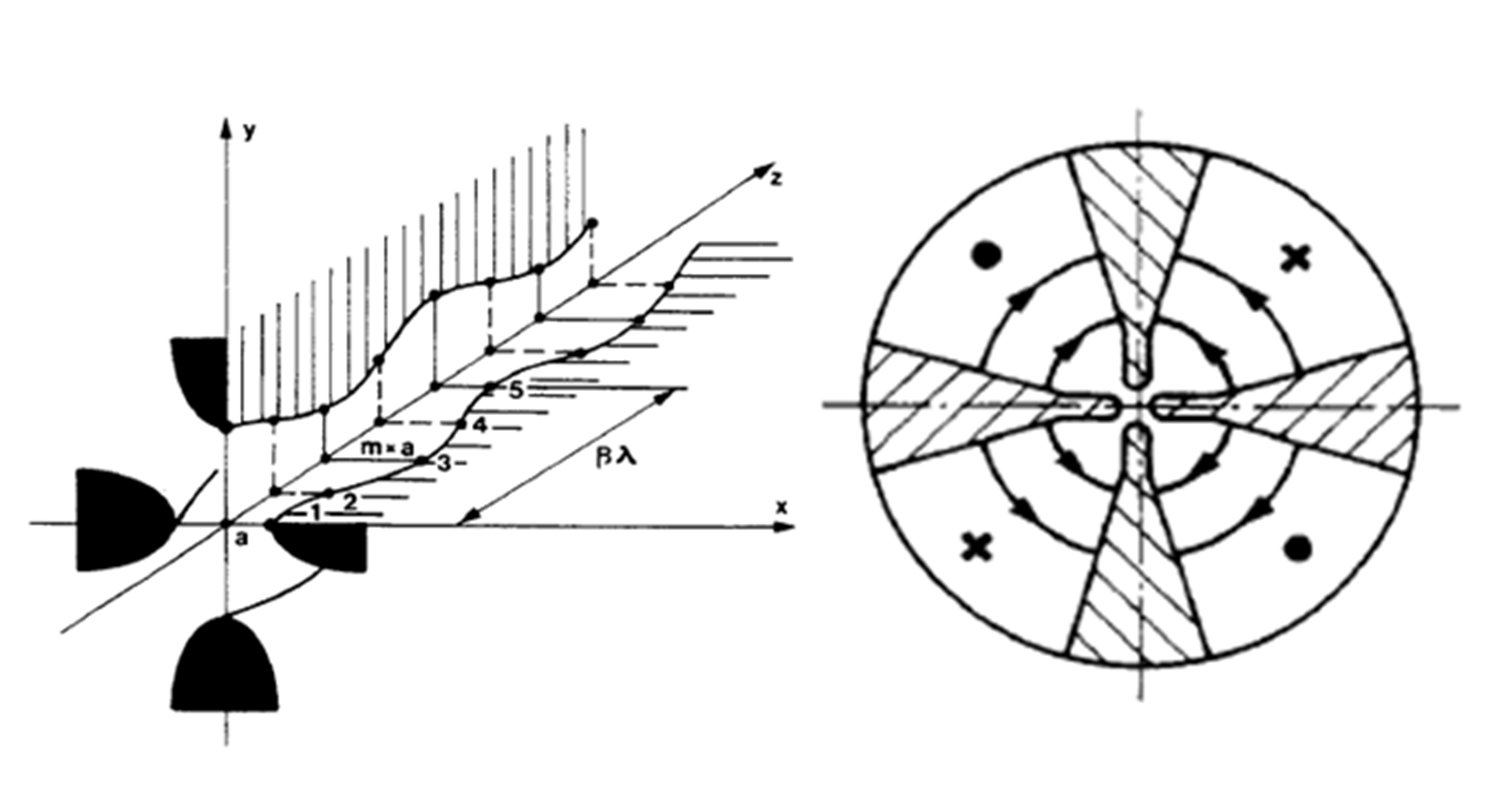
\includegraphics[width=\textwidth]{Figures/LHC_Diagrams/LHC__Linac2__RFQ_schematic.jpg}
        \caption{A schematic of a RFQ, showing the modulation of the
          flanges in the longitudinal direction \cite{LHC:LHC_linac2_rfq_schematic}}\label{fig:rfq_schematic}
      \end{subfigure}
       ~ %add desired spacing between images, e. g. ~, \quad, \qquad, \hfill etc.
      % (or a blank line to force the subfigure onto a new line)
      \begin{subfigure}[h]{0.4\textwidth}
        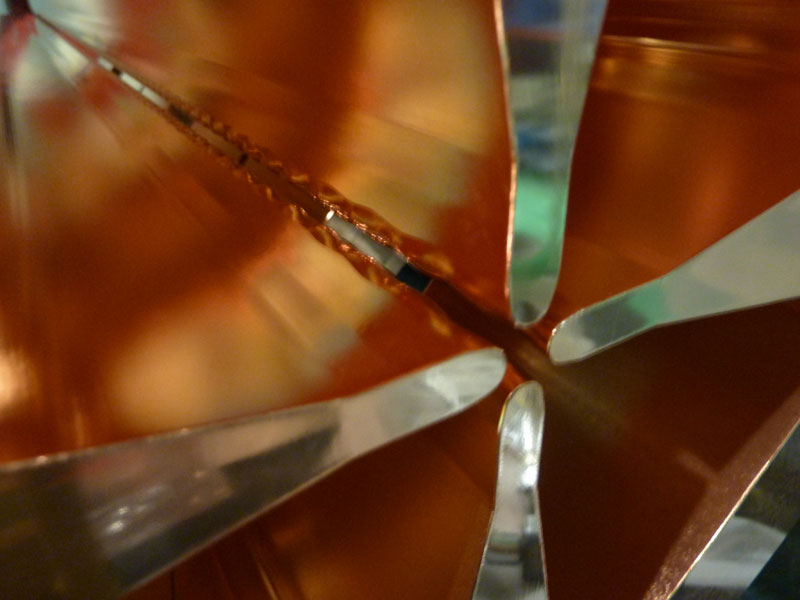
\includegraphics[width=\textwidth]{Figures/LHC_Diagrams/LHC__Linac2__RFQ.jpg}
        \caption{A close-up image of a RFQ, showing the precise
          machining of the longitudinal modulation of the flanges \cite{LHC:LHC_linac2_rfq_image}}\label{fig:rfq_actual}
      \end{subfigure}
      ~ %add desired spacing between images, e. g. ~, \quad, \qquad, \hfill etc.
      % (or a blank line to force the subfigure onto a new line)
      \begin{subfigure}[h]{0.4\textwidth}
        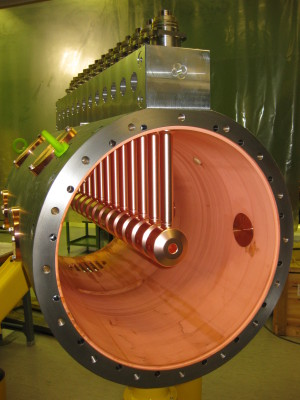
\includegraphics[width=\textwidth]{Figures/LHC_Diagrams/LHC__Linac2__AlvarezTube_Inside__DTL_proto_assembled_image.jpg}
        \caption{The inside of an Alvarez tank, showing the central
          drift tubes, where the protons are accelerated at each gap
          between successive drift tubes \cite{LHC:LHC_linac2_alvarezChambersInside_image}}\label{fig:alvarez_tank_inside}
      \end{subfigure}
      ~ %add desired spacing between images, e. g. ~, \quad, \qquad, \hfill etc.
      % (or a blank line to force the subfigure onto a new line)
      \begin{subfigure}[h]{0.4\textwidth}
        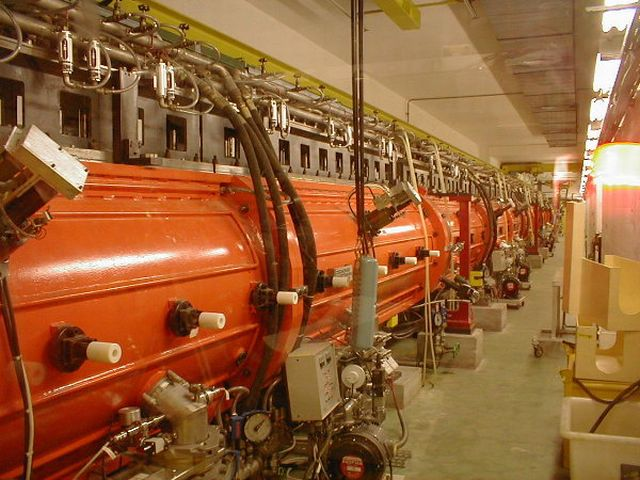
\includegraphics[width=\textwidth]{Figures/LHC_Diagrams/LHC__Linac2__AlvarezTubes.jpg}
        \caption{The Alvarez tanks at the Linac2 \cite{LHC:LHC_linac2_alvarezChambers_image}}\label{fig:alvarez_tank_actual}
      \end{subfigure}
      \caption{Features of the Linac2, the first stage of
        acceleration in the LHC injection chain} \label{fig:linac2}
\end{figure}

\par Protons are initially accelerated by the Linac2 linear accelerator
up to 50
\MeV~\cite{LHC:TDR_Vol3_InjectionChain_Benedikt}~\cite{LHC:LHIC_linac2_lhcTests_Hill}.
A bottle of Hydrogen is attached to a duoplasmatron source.  This
device ionizes the Hydrogen, and creates a 300 mA beam of protons,
through a high-voltage anode, and a geometry designed to focus and
collimate the beam as it leaves the device.  Figure
\ref{fig:linac2}(\subref{fig:duoplasmatron_schematic}) shows a
schematic for this device, showing the gas input on the left, and
proton beam leaving to the right.  Figure
\ref{fig:linac2}(\subref{fig:duoplasmatron_actual}) shows the actual
device used in the Linac2 at CERN.  The proton beam then enters the
Radio-Frequency Quadrupole (RFQ) system, which accelerates and bunches
the protons up to 750 keV.  The RFQ is a waveguide with four flanges,
which have been machined with a sinusoidal modulation in the
longitudinal direction, which creates an standing electric wave in
this direction, accelerating the protons.  Figure
\ref{fig:linac2}(\subref{fig:rfq_schematic}) shows a schematic of this
modulation, and figure \ref{fig:linac2}(\subref{fig:rfq_actual}) is a
close-up image of this modulation in an actual RFQ. The last stage of
acceleration is provided by three Alvarez tanks.  Each Alvarez tank
holds a series of electrically isolated cylinders, known as drift
tubes, coaxial with the main tank, with gaps in between them. An
alternating electric field is present in the gaps, and space between
each drift tube and the walls of the tank.  Protons passing through
the center of the drift tubes feel no electric field, but the gaps are
located such that, a proton will always see an accelerating field in
the gap, and are thus receive a boost of energy from each gap as it
traverses the length of the three tanks.  Figure
\ref{fig:linac2}(\subref{fig:alvarez_tank_inside}) shows an image of
the inside of an Alvarez tank, and figure
\ref{fig:linac2}(\subref{fig:alvarez_tank_actual}) shows the tanks at
the Linac2 at CERN.  The final product is a 180 mA, 50 \MeV proton
beam, which is steered to the Proton Synchrotron Booster for the next
stage of acceleration.

\begin{figure}{h}
    \centering
    \begin{subfigure}[h]{0.4\textwidth}
        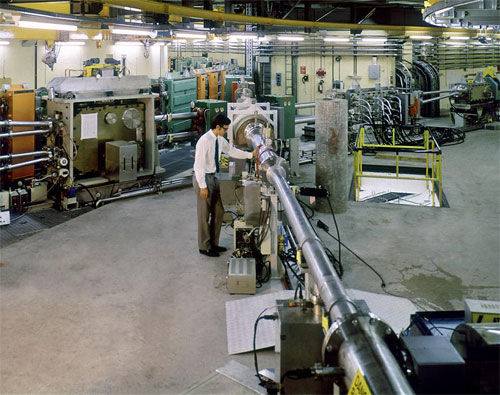
\includegraphics[width=\textwidth]{Figures/LHC_Diagrams/LHC__PSbooster__psb_injection.jpg}
        \caption{The Injection site from the Linac2 into the PS booster
        \cite{LHC:LHC_psbooster_injection_image}}\label{fig:linac2_to_psbooster_injection}
      \end{subfigure}
      ~ %add desired spacing between images, e. g. ~, \quad, \qquad, \hfill etc.
      % (or a blank line to force the subfigure onto a new line)
      \begin{subfigure}[h]{0.4\textwidth}
        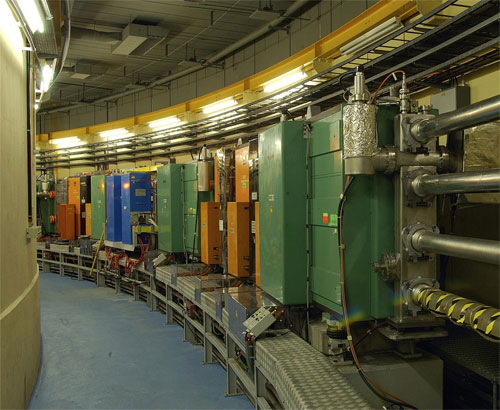
\includegraphics[width=\textwidth]{Figures/LHC_Diagrams/LHC__PSbooster__psb_4_beamLines_shown.jpg}
        \caption{A section of the PS booster, with the four stack
          synchrotron beam-lines shown in the lower right hand side of
          the picture \cite{LHC:LHC_psbooster_4stacks_image}}\label{fig:psbooster_4stacks}
      \end{subfigure}
       ~ %add desired spacing between images, e. g. ~, \quad, \qquad, \hfill etc.
      % (or a blank line to force the subfigure onto a new line)
      \begin{subfigure}[h]{0.4\textwidth}
        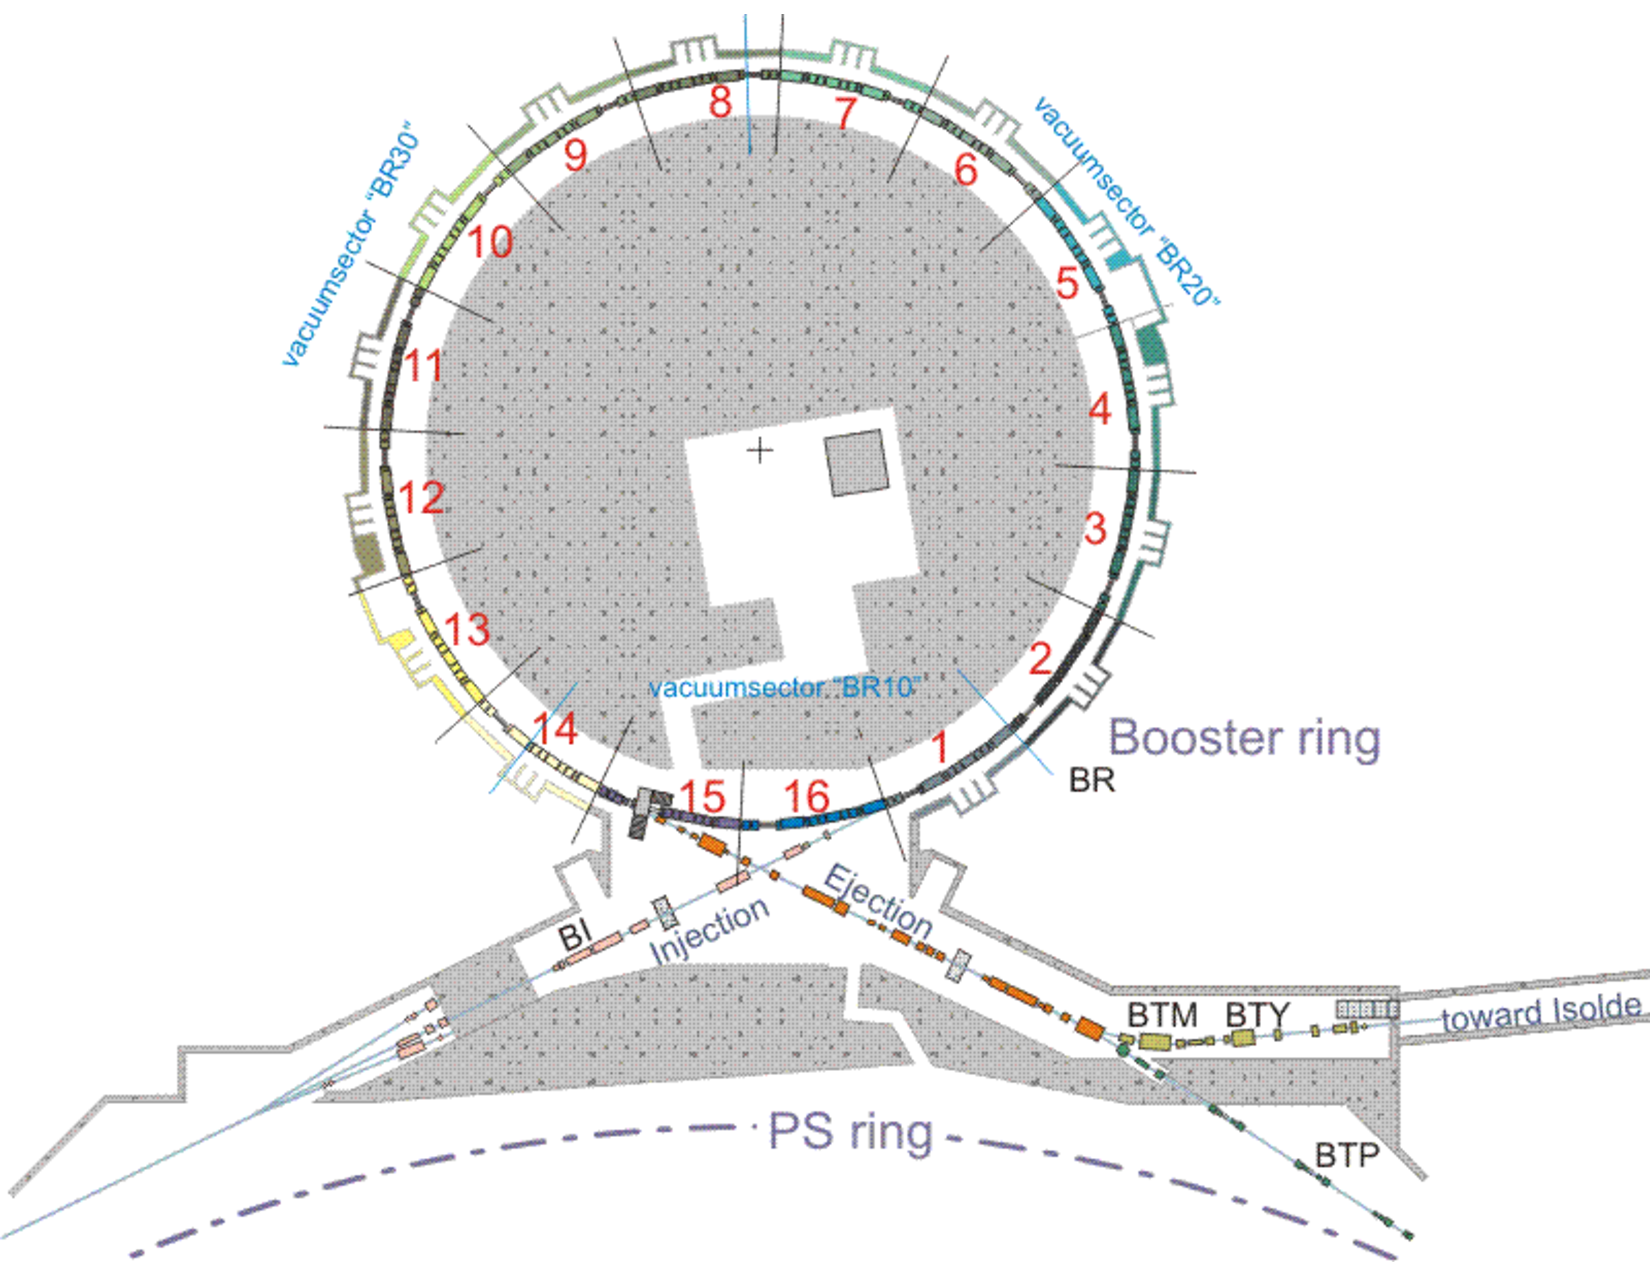
\includegraphics[width=\textwidth]{Figures/LHC_Diagrams/LHC__PSbooster__Layout.pdf}
        \caption{A drawing of the 16 sections of the PS booster \cite{LHC:LHC_psbooster_layout_image}}\label{fig:psbooster_16sections}
      \end{subfigure}
       ~ %add desired spacing between images, e. g. ~, \quad, \qquad, \hfill etc.
      % (or a blank line to force the subfigure onto a new line)
      \begin{subfigure}[h]{0.4\textwidth}
        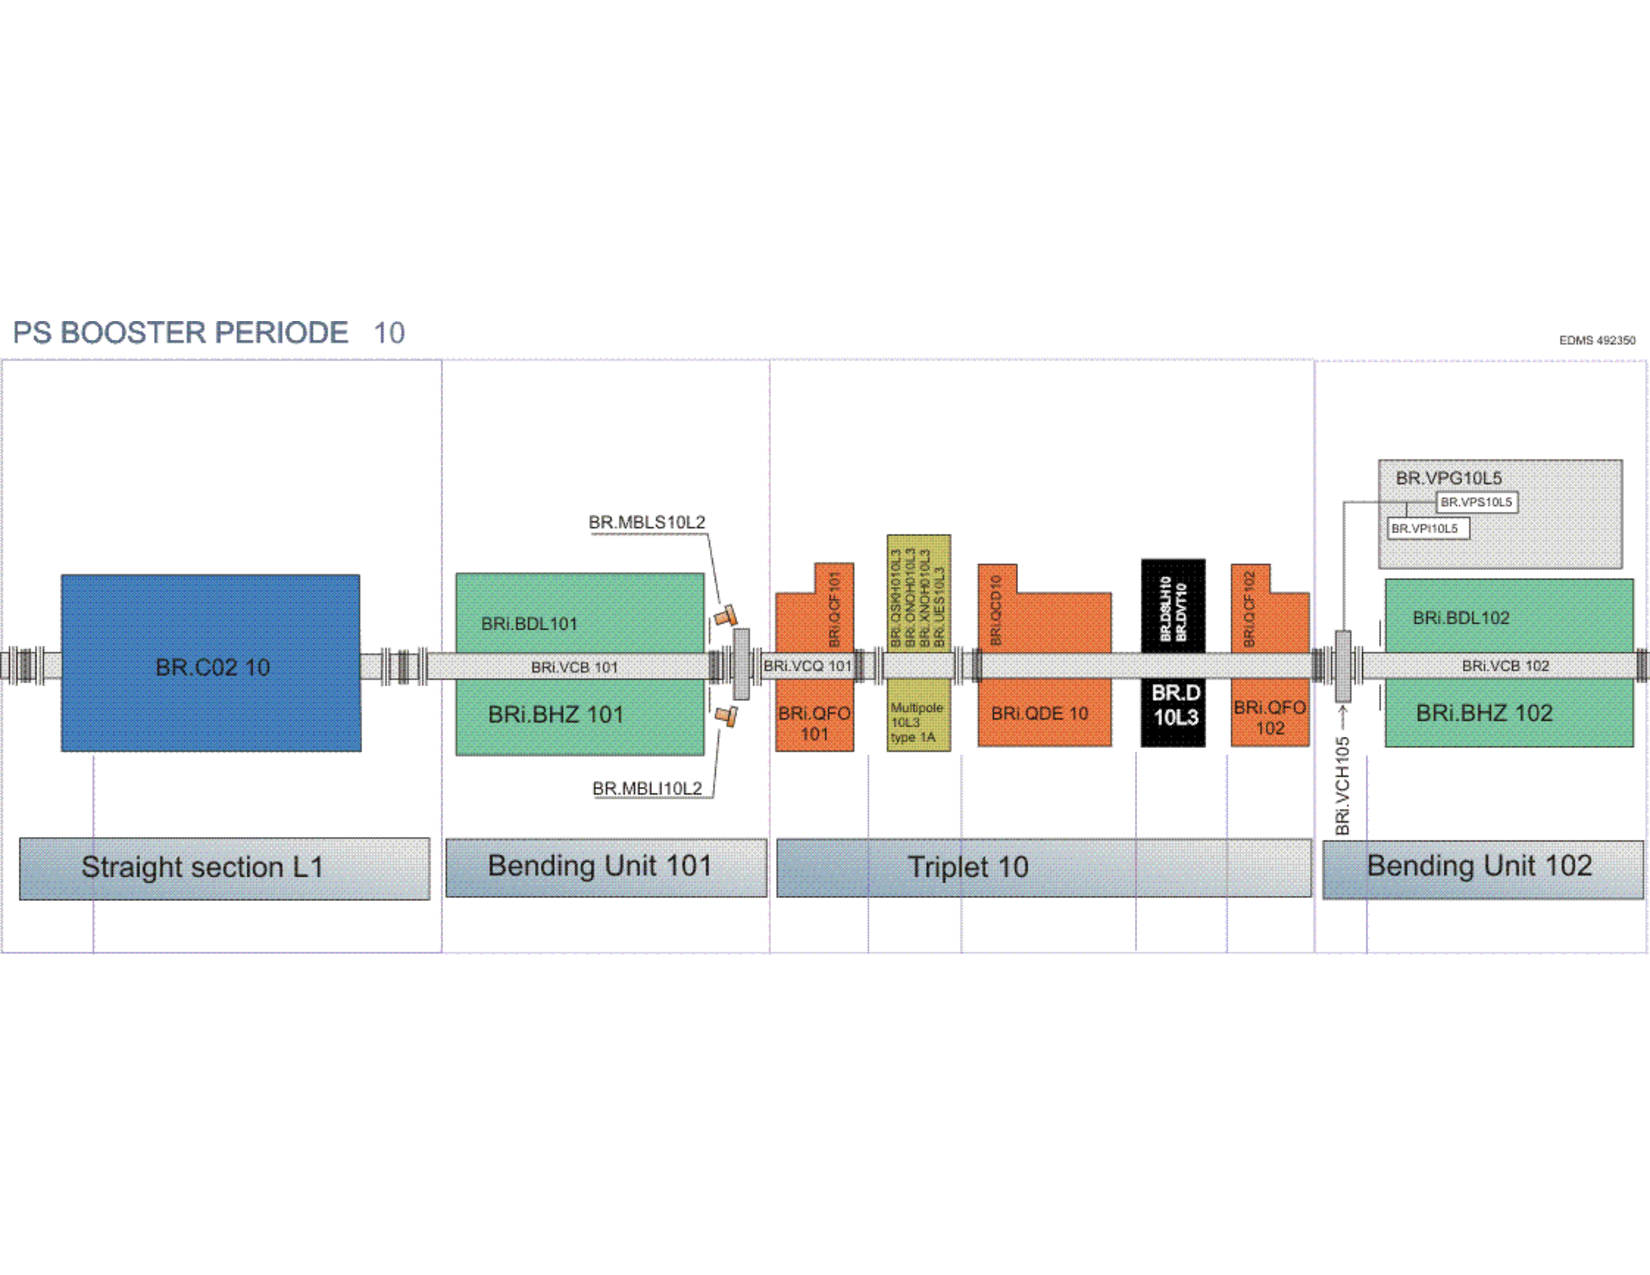
\includegraphics[width=\textwidth]{Figures/LHC_Diagrams/LHC__PSbooster__sect10.pdf}
        \caption{Section 10 of the PS booster.  This begins with the
          CO2 cavity, the main driver of the acceleration; followed by
        a dipole magnet, a triplet of focusing magnets, and a second
        dipole magnet \cite{LHC:LHC_psbooster_section10_layout_image}}\label{fig:psbooster_section10}
      \end{subfigure}
      ~ %add desired spacing between images, e. g. ~, \quad, \qquad, \hfill etc.
      % (or a blank line to force the subfigure onto a new line)
      \begin{subfigure}[h]{0.4\textwidth}
        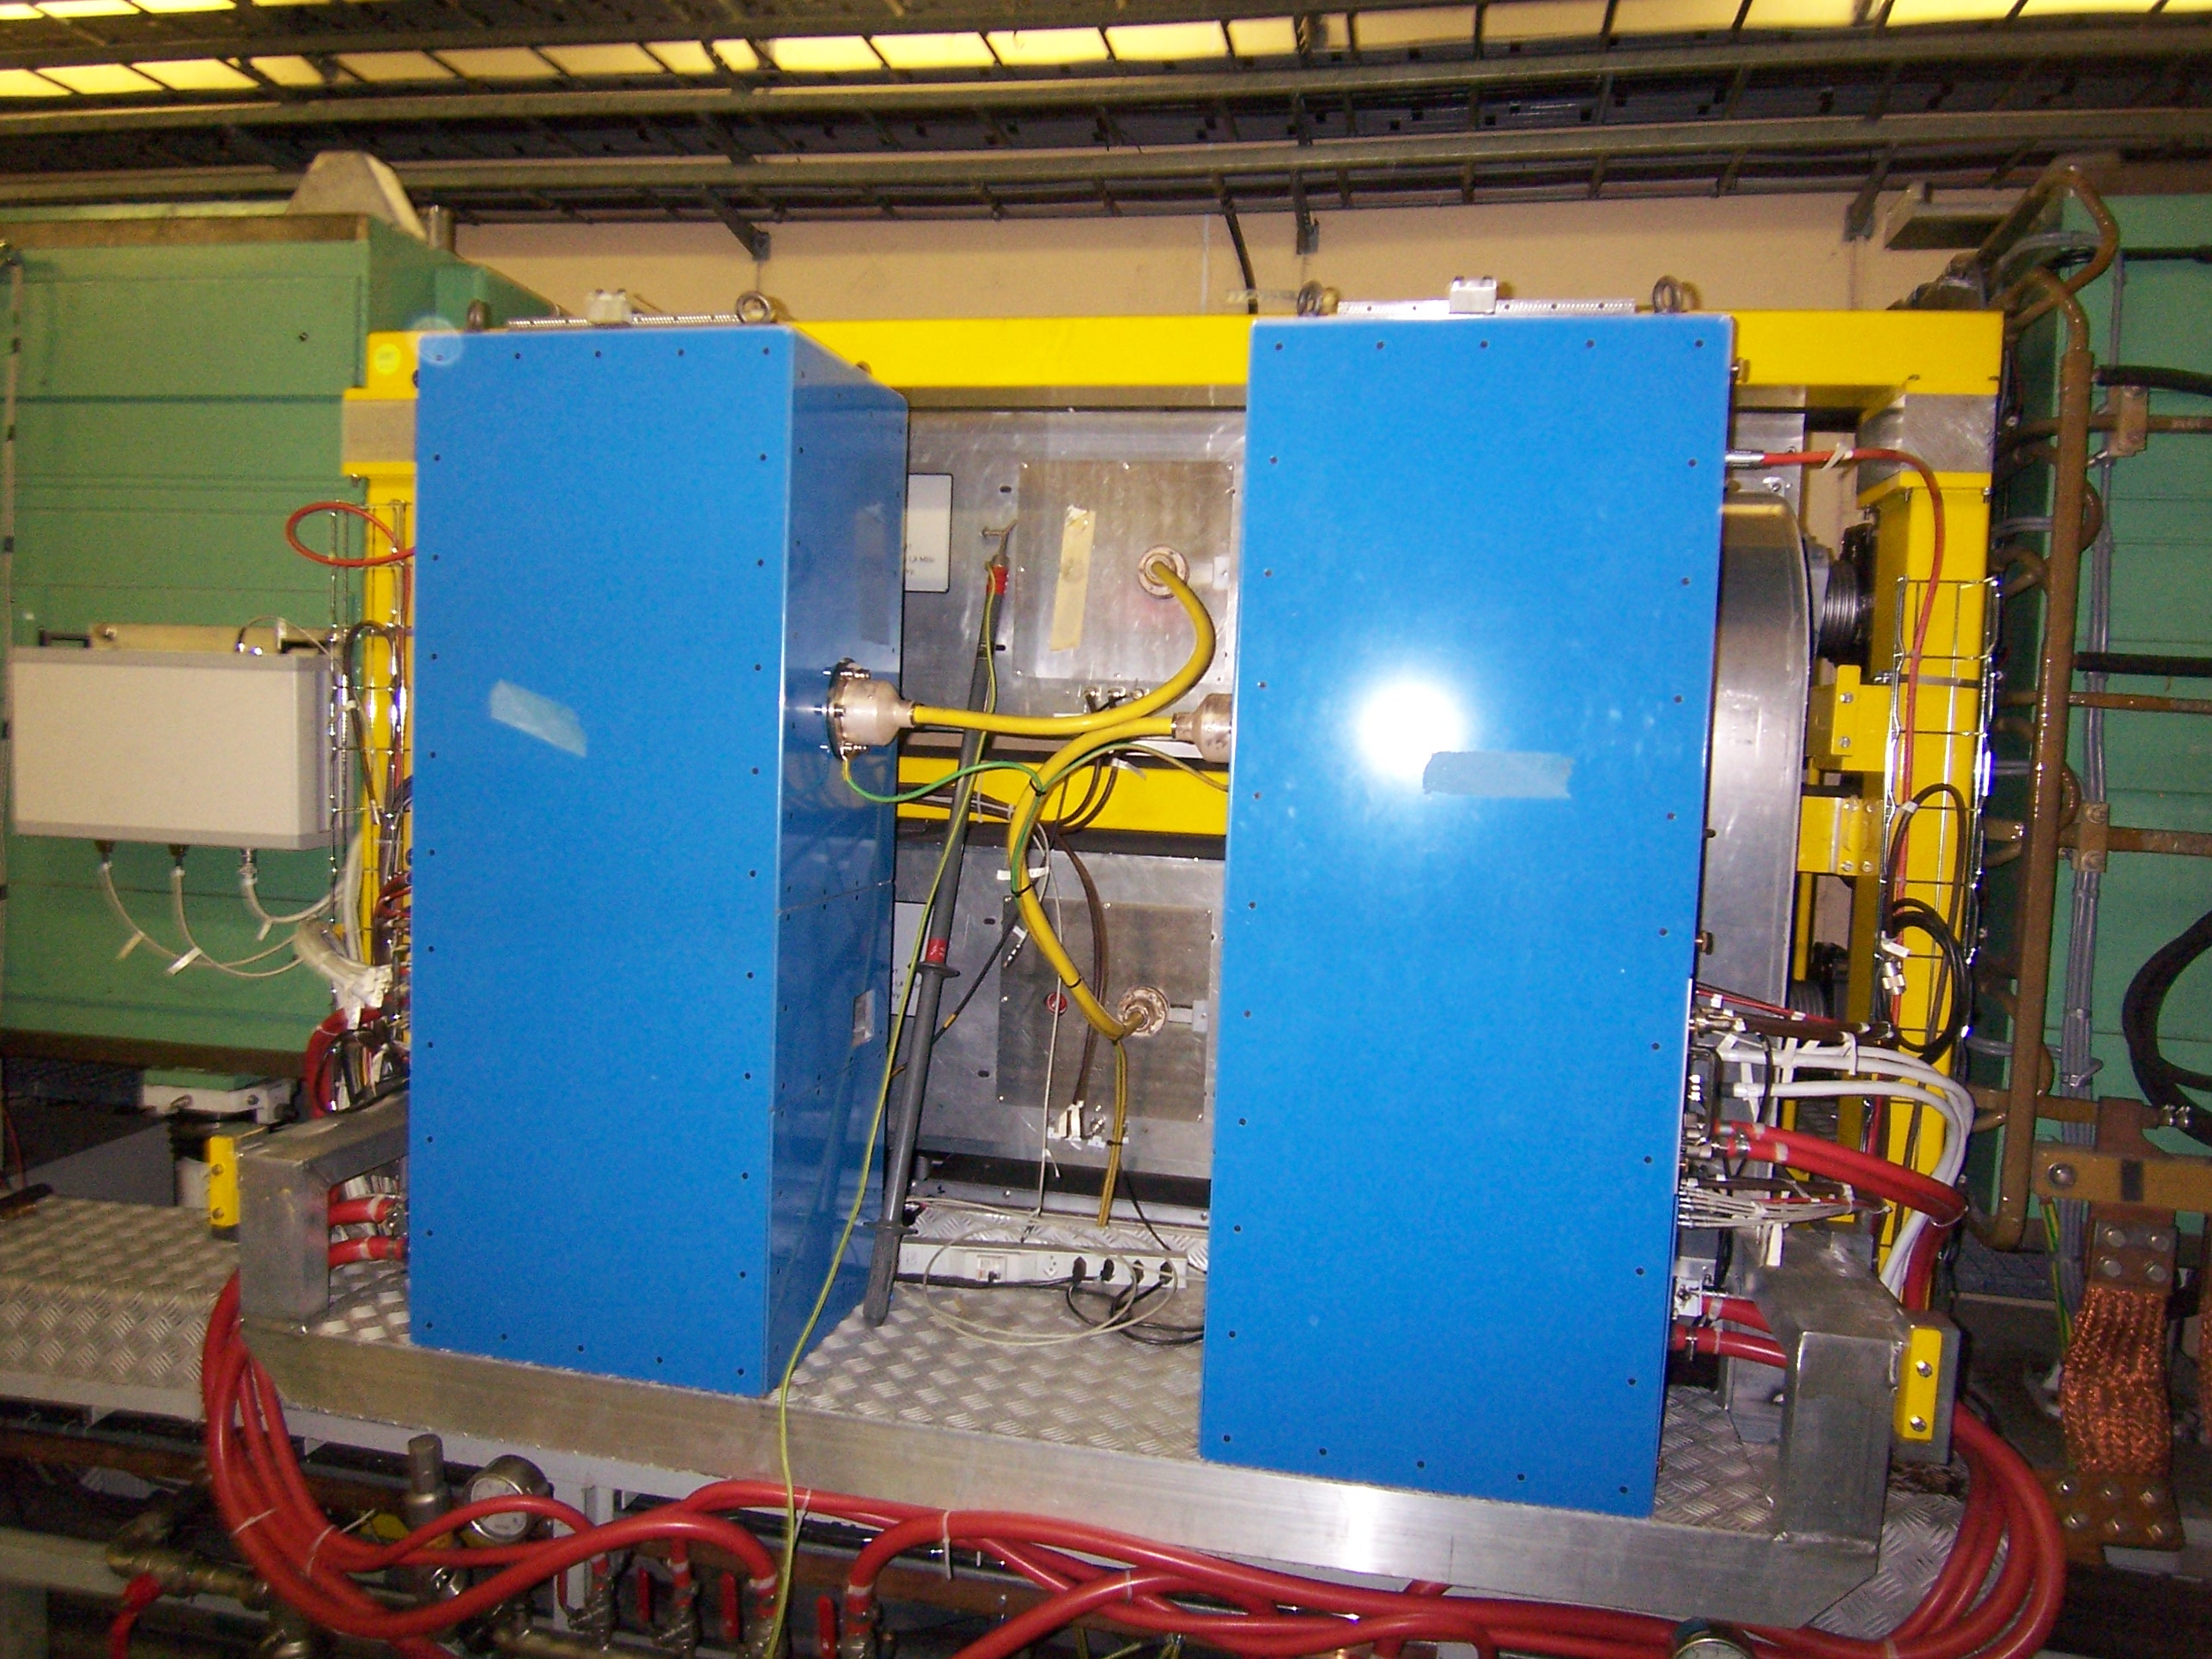
\includegraphics[width=\textwidth]{Figures/LHC_Diagrams/LHC__PSbooster__CO2_RFCavity__P10L1.JPG}
        \caption{A picture of the CO2 RF Cavity, which provides the
          principle acceleration for the protons in the PS booster \cite{LHC:LHC_psbooster_CO2_RF_Cavity_image}}\label{fig:psbooster_CO2_RFCavity}
      \end{subfigure}
      ~ %add desired spacing between images, e. g. ~, \quad, \qquad, \hfill etc.
      % (or a blank line to force the subfigure onto a new line)
      \begin{subfigure}[h]{0.4\textwidth}
        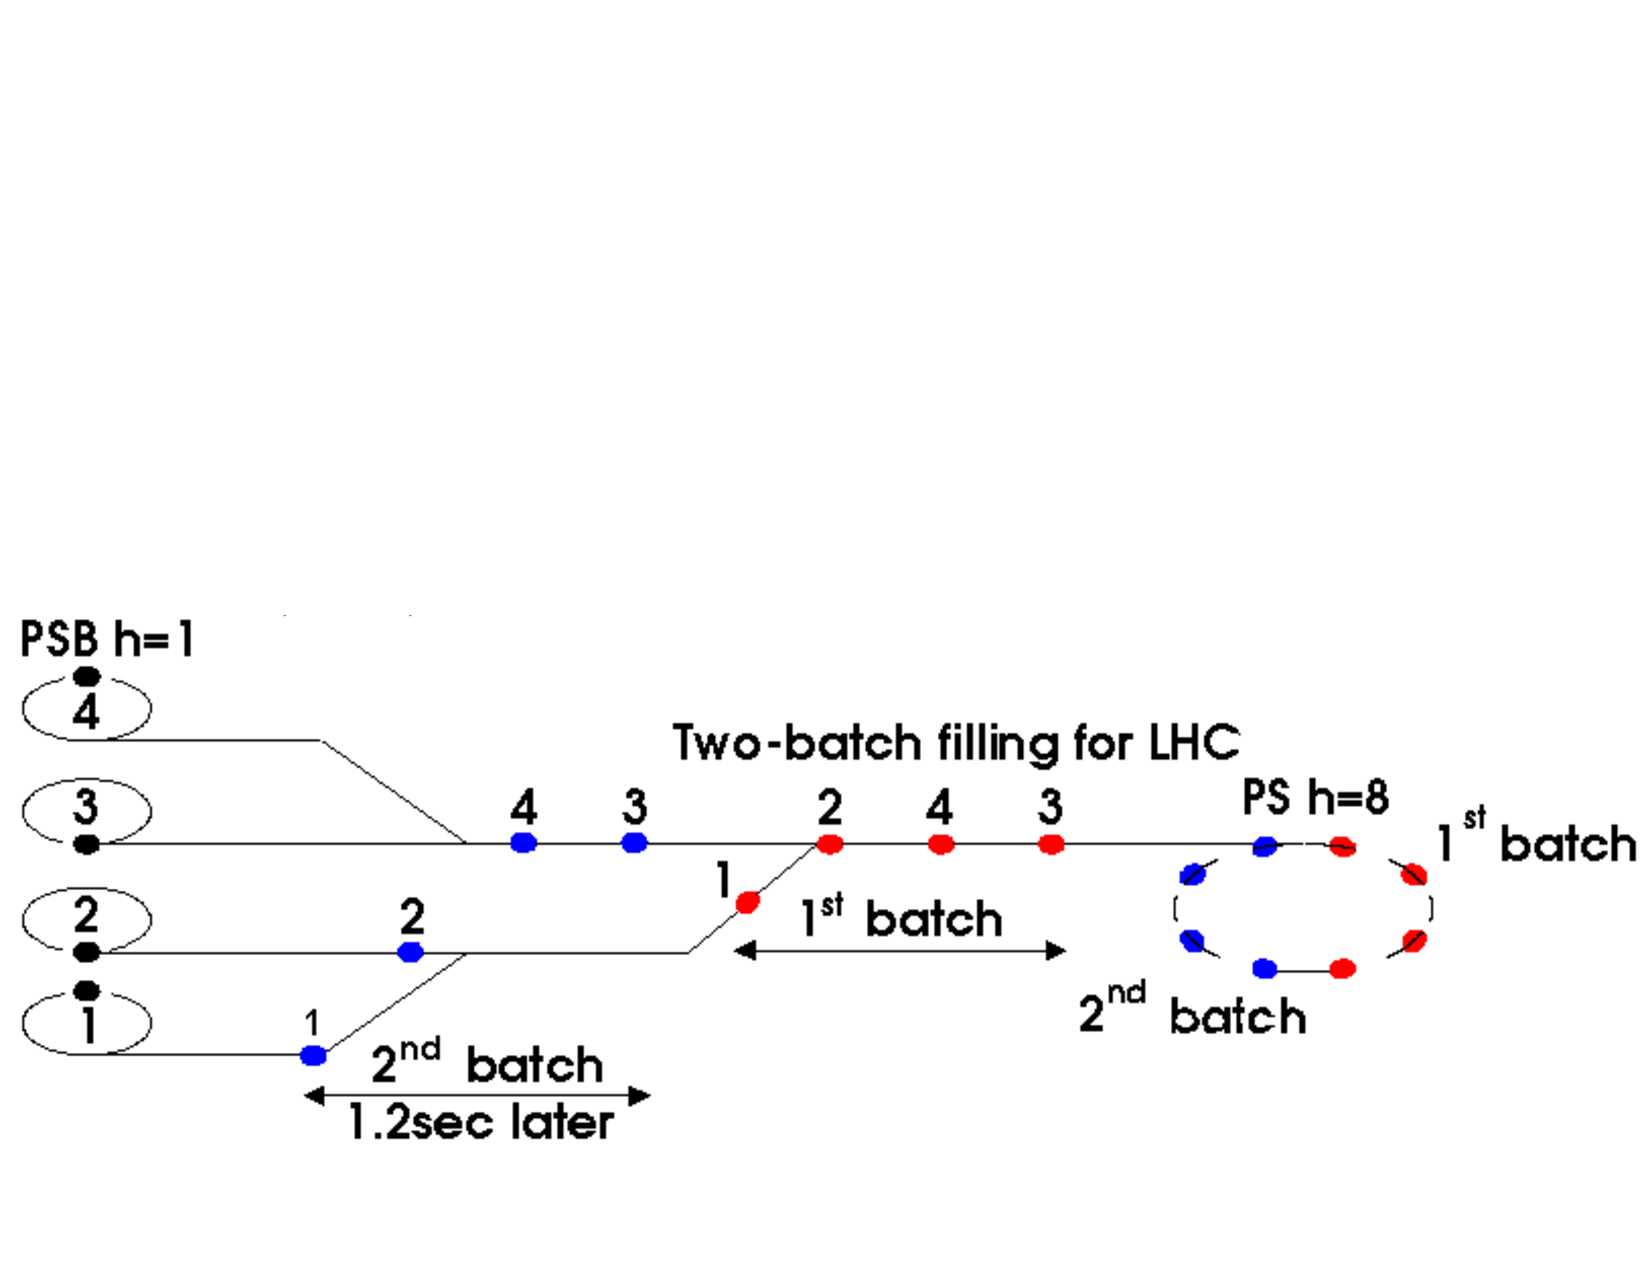
\includegraphics[width=\textwidth]{Figures/LHC_Diagrams/LHC__PSbooster__2batchFillingScheme__schindlrf.pdf}
        \caption{The two batch filling scheme for the PS.  It takes
          1.2 s for each batch to be accelerated from 50 \MeV to 1.4
          \GeV \cite{LHC:LHC_psbooster_2batchScheme_image}}\label{fig:psbooster_2batchScheme}
      \end{subfigure}
      \caption{Features of the PS booster, the second stage of
        the LHC injection chain}\label{fig:psbooster}
\end{figure}

\par The Proton Synchrotron Booster (PS booster) complex accelerates
the protons up to 1.4
\GeV~\cite{LHC:TDR_Vol3_InjectionChain_Benedikt}.  The complex takes
the proton beam from the Linac2 and splits the beam into four
separate, synchrotrons, stacked on top of one another.  Figure
\ref{fig:psbooster}(\subref{fig:linac2_to_psbooster_injection}) shows the
injection site of the proton beam from the Linac2 into the PS booster.
The right side of figure
\ref{fig:psbooster}(\subref{fig:psbooster_4stacks}) shows the four
synchrotron beam pipes stacked vertically on top one another.  The
splitting of the beam is done in order to reduce the effect of the
space charge of the proton beam, which would increase the transverse
emmitance beyond a tolerable degree.  The PS booster uses thirty-two
0.87 T dipole magnets to bend the beams, and fourty-eight quadrupoles
to focus the beam as it makes its way around each of the 50 m diameter
rings.  Each magnet is composed of a vertical stack of four magnets,
one for each of the synchrotrons, and share a common yoke, allowing one
power supply to provide the current to all of them in 
series~\cite{LHC:LHC_psbooster_boosterTurns40}.  The booster is
divided into 16 arcs, as shown in figure
\ref{fig:psbooster}(\subref{fig:psbooster_16sections}).  Each arc contains
a bending dipole, 3 focusing quadrupoles, and a second bending dipole,
followed by a straight section containing beam diagnostic, injection
and ejection systems, and in three sections, the Radio-Frequency (RF) cavities, which is
the mechanism of accelerating the
beam~\cite{LHC:LHC_psbooster_layout}.  Figure
\ref{fig:psbooster}(\subref{fig:psbooster_section10}) shows the layout
of the tenth arc, which also contains one of the RF cavities in the first
section.
  
\par An RF cavity is a specially shaped, hollow
conductor, that the beam passes
through~\cite{LHC:BasicsOfAccelerators_Baird}.  The shape of the
cavity determines the resonant frequency and harmonics (integer
multiples of the fundamental frequency), of the standing
electromagnetic fields that result when the cavity is driven by an
alternating voltage source.  The idea is to choose a resonant
frequency such that the proton will always experience a positive
electric field, and thus an acceleration, each time it passes through
the RF cavity.  This means that the revolution frequency of the proton
must be equal to the fundamental frequency or harmonic of the RF
cavity, $f_{RF} = n{\times}f_{rev}$, with $n=1,2,3...$.  Eventually,
the proton is accelerated up to an equilibrium speed and will enter the
cavity just as the standing electric field is alternating through it's
zero point.  If arrives too early for this (moving too fast), then it
will experience a negative electric force, a deceleration, which will
eventually bring it back to the equilibrium revolution frequency,
where it experiences zero net force.  A diffuse beam of protons will
be bunched into groups of protons through this effect as well, as the
faster protons in the beams are decelerated, and the slower ones
accelerated, until they all reach the same equilibrium revolution
frequency.  Driving  the RF cavity with a harmonic, n, of the proton's
revolution speed will thus create n bunches of protons.  Each one of
the potential n bunch positions is referred to as a bucket.  In the
case where a proton has to be accelerated through a wide range of
energies, the frequency of the cavity must also increase to maintain
synchronization with the proton revolution frequency.  

\par Three types of RF cavities are used to accelerate the beam
during each revolution.  The first of the three types of RF cavities
is the CO2, with frequency range of 0.6 to 2.0 MHz and is used to
drive the $h=1$ harmonic of the  synchrotron, and is pictured in
figure \ref{fig:psbooster}(\subref{fig:psbooster_CO2_RFCavity}).  The
second type of cavity is the CO4 chamber, with a frequency range of
1.2 to 3.9 MHz, and drives the $h=2$ mode of the synchrotron.  This
second mode is capable of splitting the beam and creating two separate
bunch  structures.  However, for LHC running, only one bunch is used,
and is driven primarily by the $h=1$ mode.  The $h=2$ mode is
supplemental and is used to shape the beam.  A third type of RF
cavity, CO16, has a frequency range of 5 to 16 MHz, and is used to
control the longitudinal shape of a bunch during acceleration. The beam
leaves the PS booster and enters the PS in a two-batch filling scheme,
taking only 1.2 s to accelerate a second batch of protons from 50 \MeV
to 1.4 \GeV.  This second batch enters just as the first batch has
traveled to the opposite side of the PS ring.  A schematic of this
process is shown in figure
\ref{fig:psbooster}(\subref{fig:psbooster_2batchScheme}).  To achieve
the 25 ns bunch spacing design of the LHC, only 6 bunches of proton
beam need to be delivered to PS.  This is achieved by either using a
4+2 or 3+3 filling scheme, in terms of the number of proton bunches
delivered from the four possible synchrotrons.   

\begin{figure}{h}
    \centering
    \begin{subfigure}[h]{0.45\textwidth}
        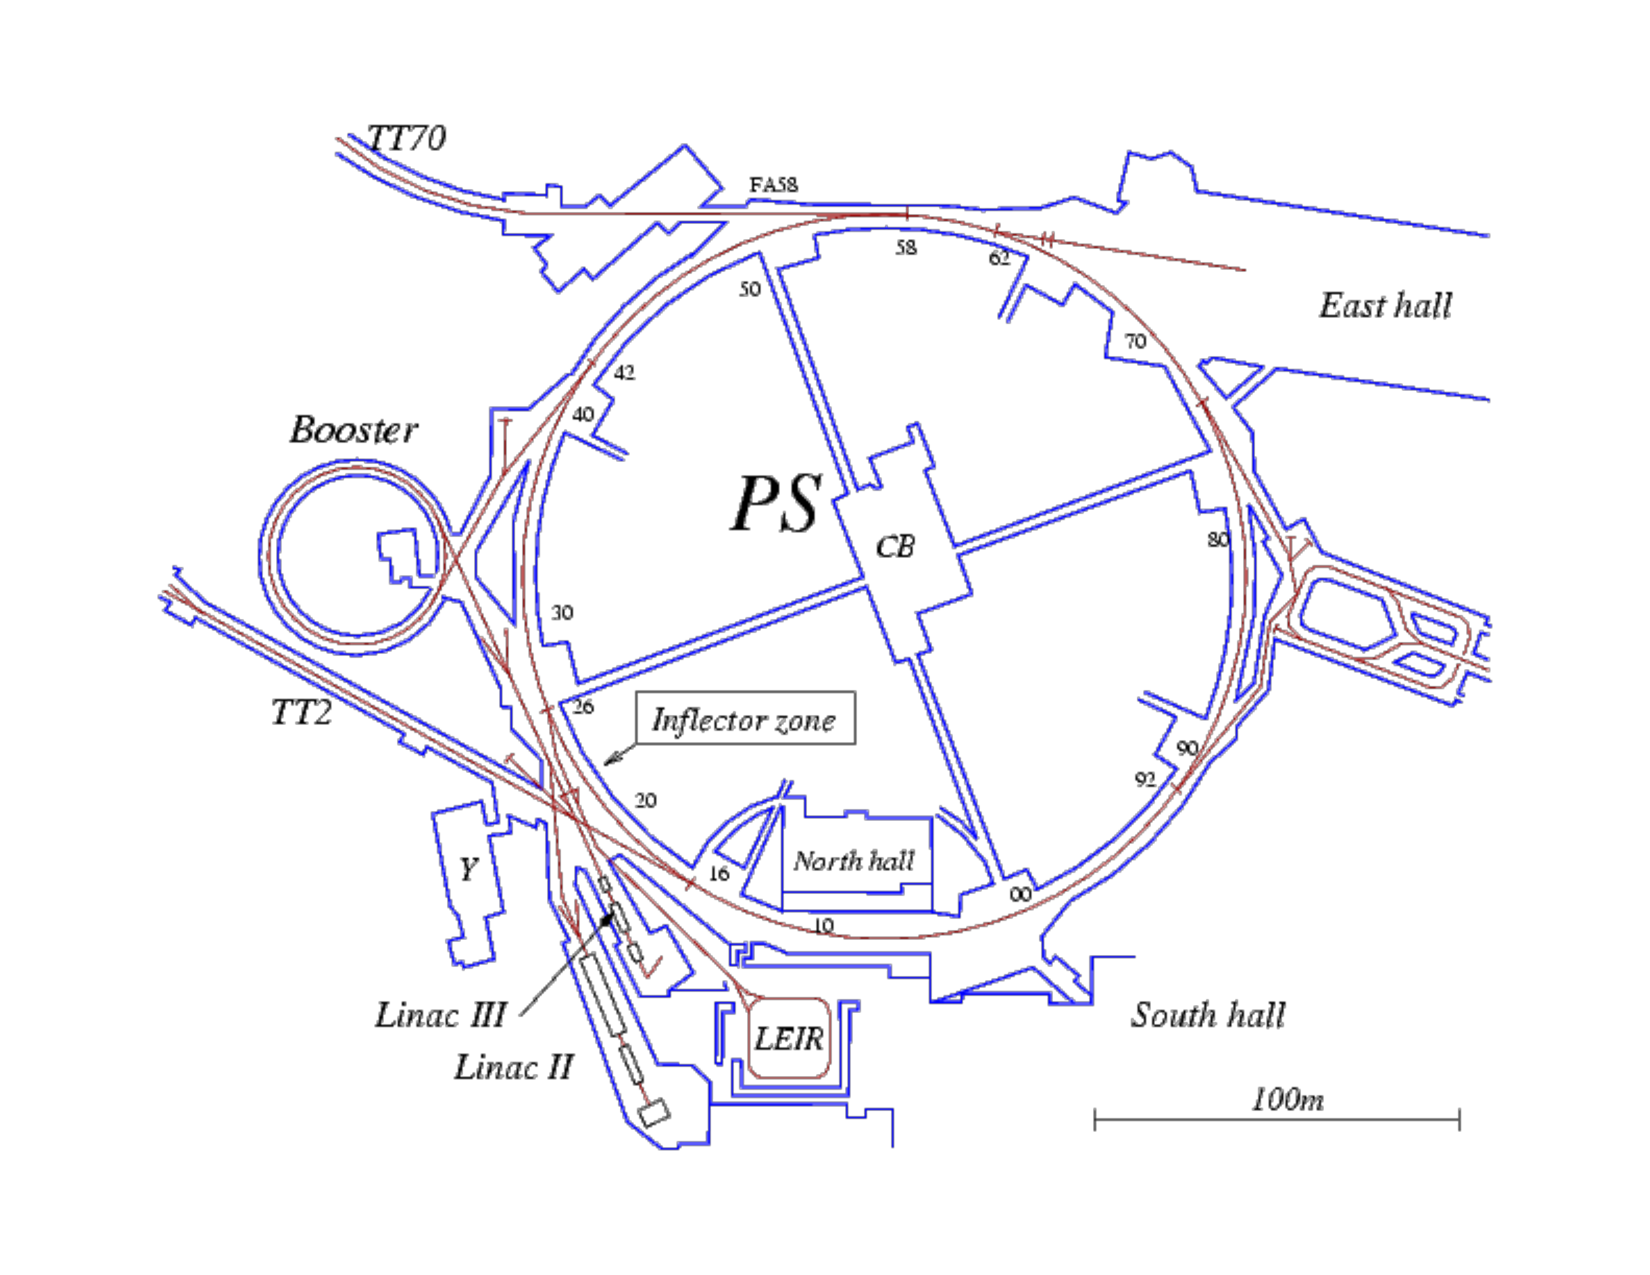
\includegraphics[width=\textwidth]{Figures/LHC_Diagrams/LHC__PS__pscomplex.pdf}
        \caption{A diagram of the PS layout \cite{LHC:LHC_ps_layout_image}}\label{fig:ps_layout}
      \end{subfigure}
      ~ %add desired spacing between images, e. g. ~, \quad, \qquad, \hfill etc.
      % (or a blank line to force the subfigure onto a new line)
    \begin{subfigure}[h]{0.45\textwidth}
        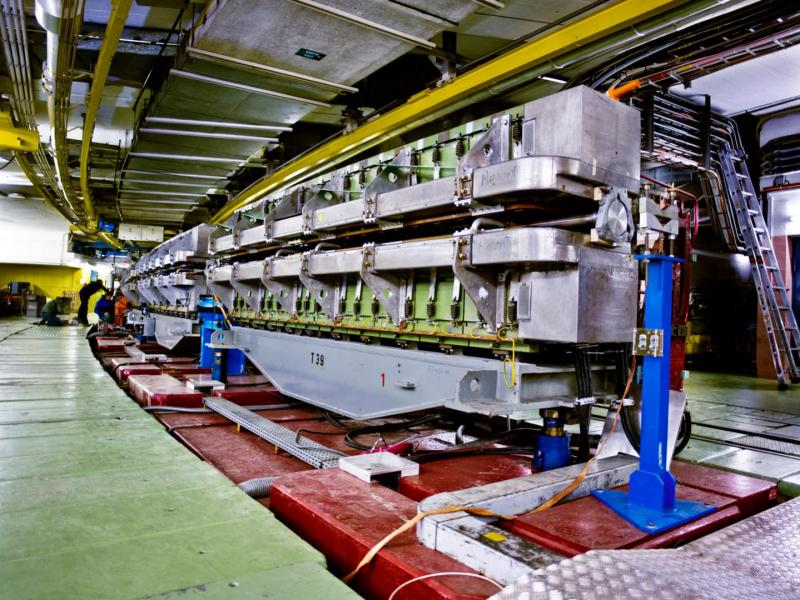
\includegraphics[width=\textwidth]{Figures/LHC_Diagrams/LHC__PS__Dipoles_accelerators-ps.jpg}
        \caption{Dipole magnets used to steer the beam around the 100
          m radius PS ring \cite{LHC:LHC_ps_dipoles_image}}\label{fig:ps_dipoles}
      \end{subfigure}
      ~ %add desired spacing between images, e. g. ~, \quad, \qquad, \hfill etc.
      % (or a blank line to force the subfigure onto a new line)
      \begin{subfigure}[h]{0.45\textwidth}
        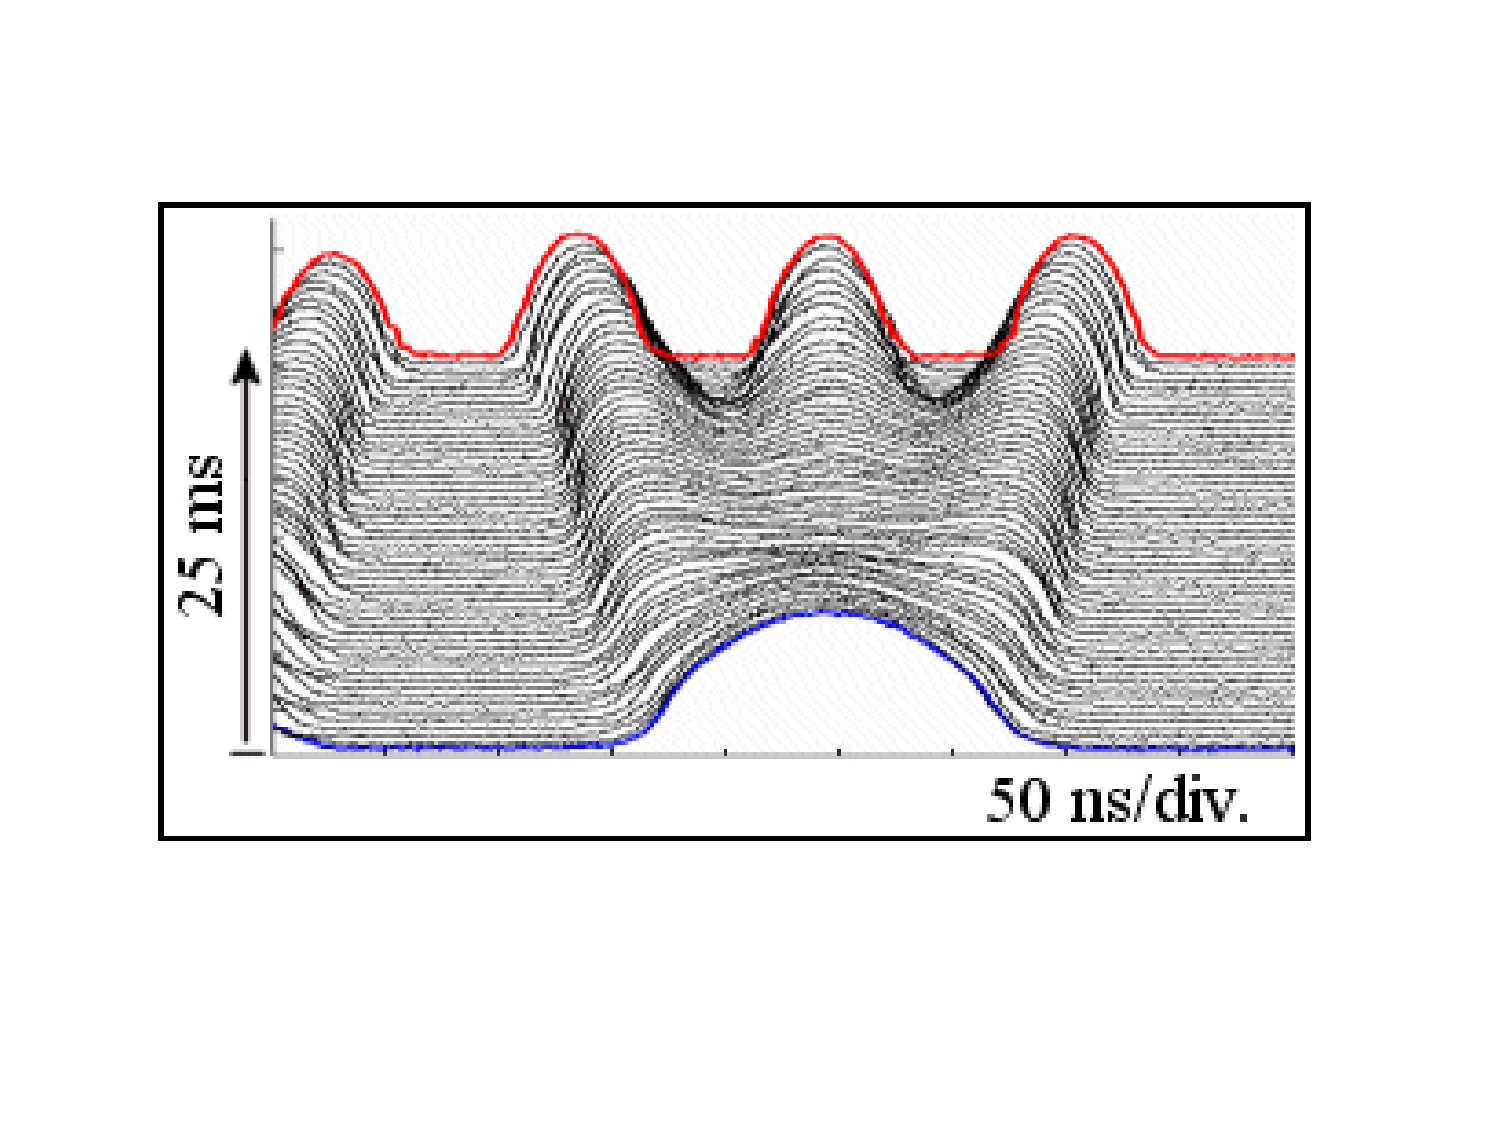
\includegraphics[width=\textwidth]{Figures/LHC_Diagrams/LHC__PS__TripleBunchSplitting.pdf}
        \caption{A simulation of the PS using the $h=7,14,21$ modes of
        to split the beam into 3 bunches \cite{LHC:TDR_Vol3_InjectionChain_Benedikt}}\label{fig:ps_split3}
      \end{subfigure}
       ~ %add desired spacing between images, e. g. ~, \quad, \qquad, \hfill etc.
      % (or a blank line to force the subfigure onto a new line)
      \begin{subfigure}[h]{0.45\textwidth}
        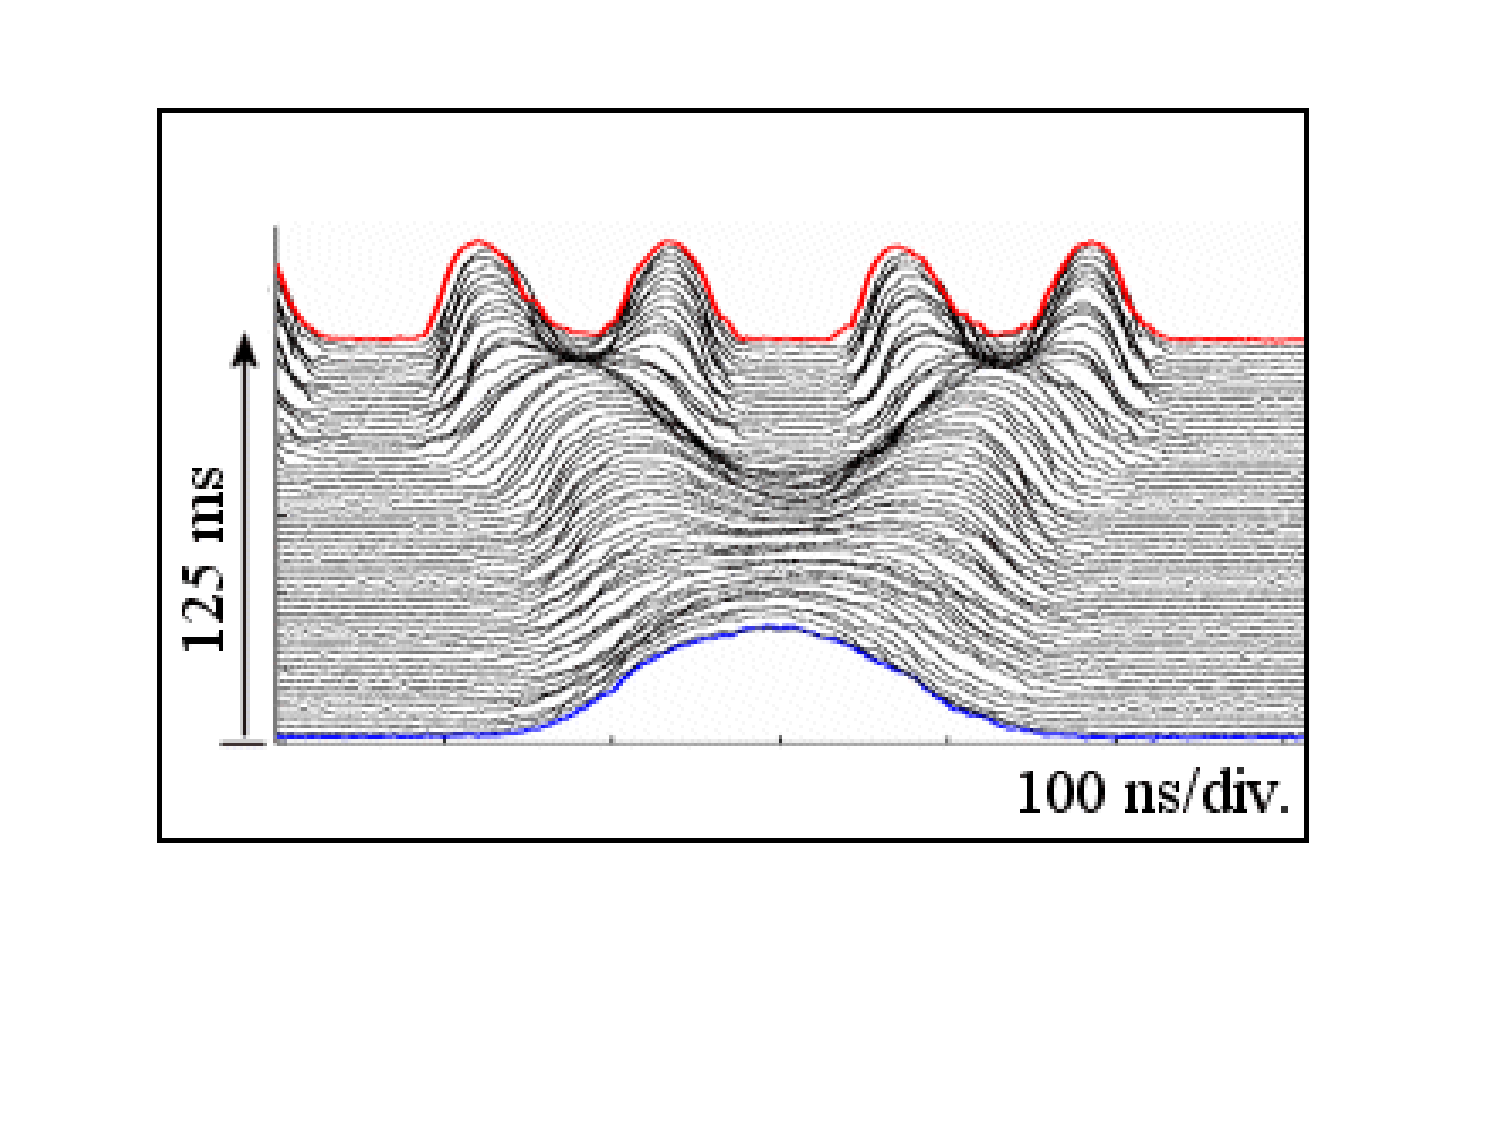
\includegraphics[width=\textwidth]{Figures/LHC_Diagrams/LHC__PS__DoubleDoubleBunchSplitting.pdf}
        \caption{A simulation of the splitting each bunch into two,
          and two again \cite{LHC:TDR_Vol3_InjectionChain_Benedikt} }\label{fig:ps_split2x2}
      \end{subfigure}
       ~ %add desired spacing between images, e. g. ~, \quad, \qquad, \hfill etc.
      % (or a blank line to force the subfigure onto a new line)
      \begin{subfigure}[h]{0.45\textwidth}
        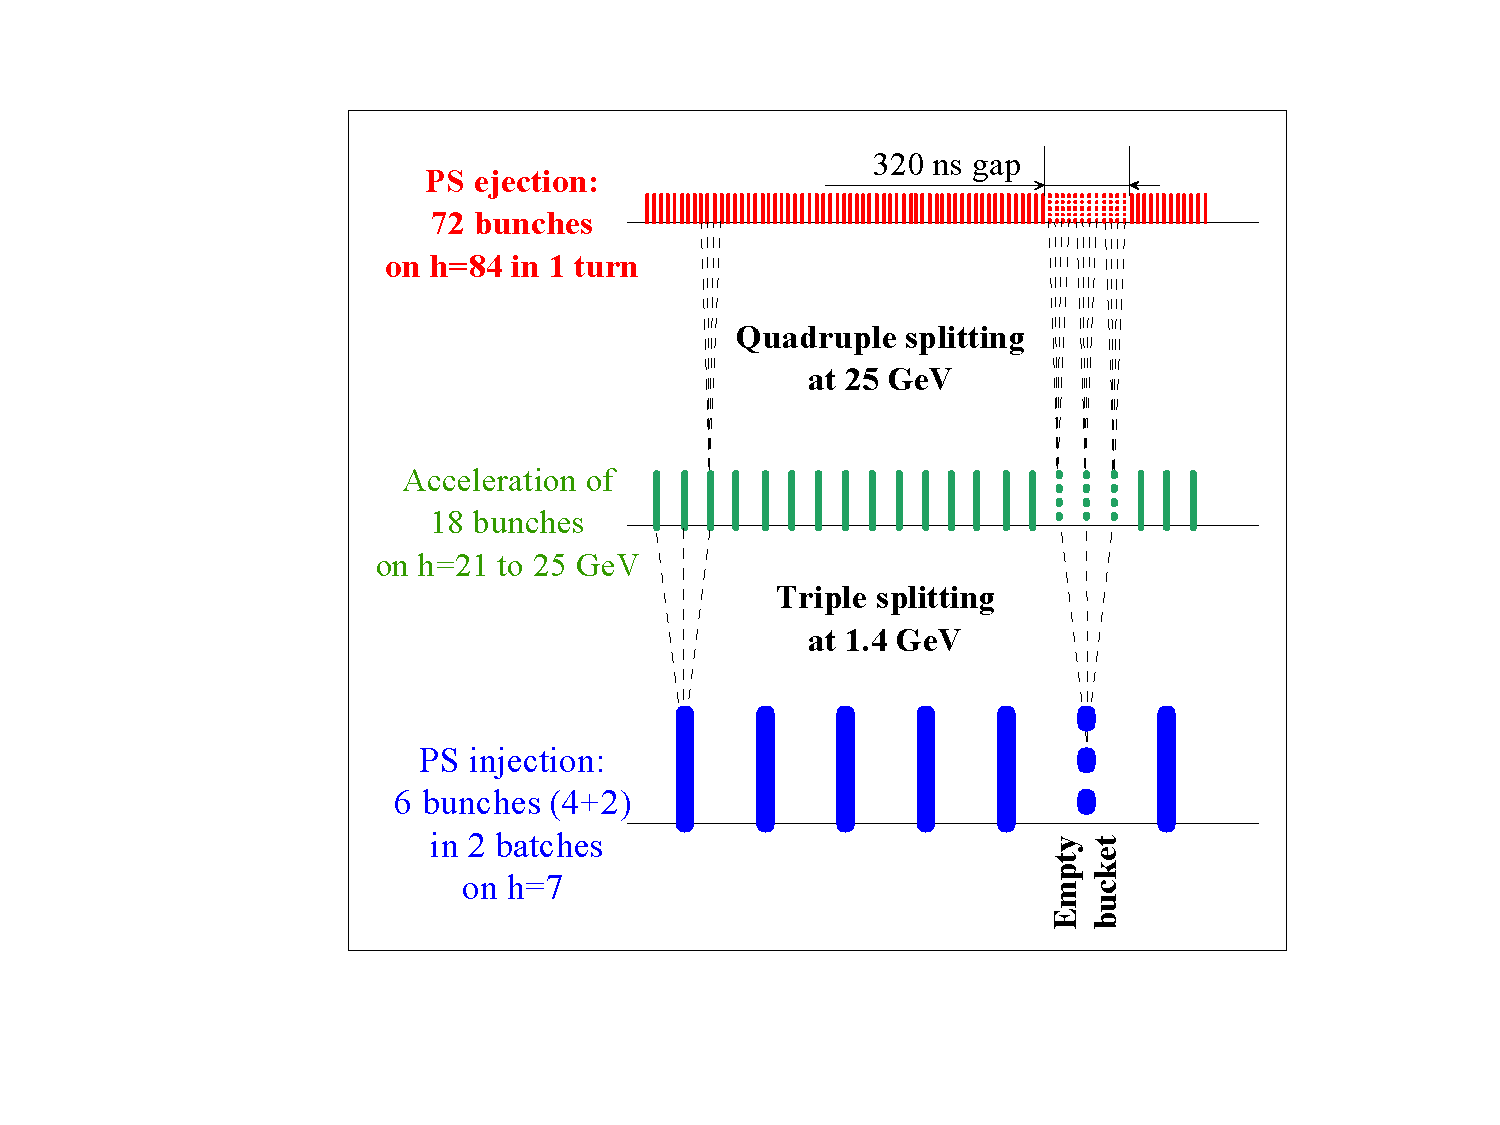
\includegraphics[width=\textwidth]{Figures/LHC_Diagrams/LHC__PS__BunchSplittingDiagram.pdf}
        \caption{An overview of the splitting procedure \cite{LHC:TDR_Vol3_InjectionChain_Benedikt}}\label{fig:ps_splitting}
      \end{subfigure}
      ~ %add desired spacing between images, e. g. ~, \quad, \qquad, \hfill etc.
      % (or a blank line to force the subfigure onto a new line)
      \begin{subfigure}[h]{0.45\textwidth}
        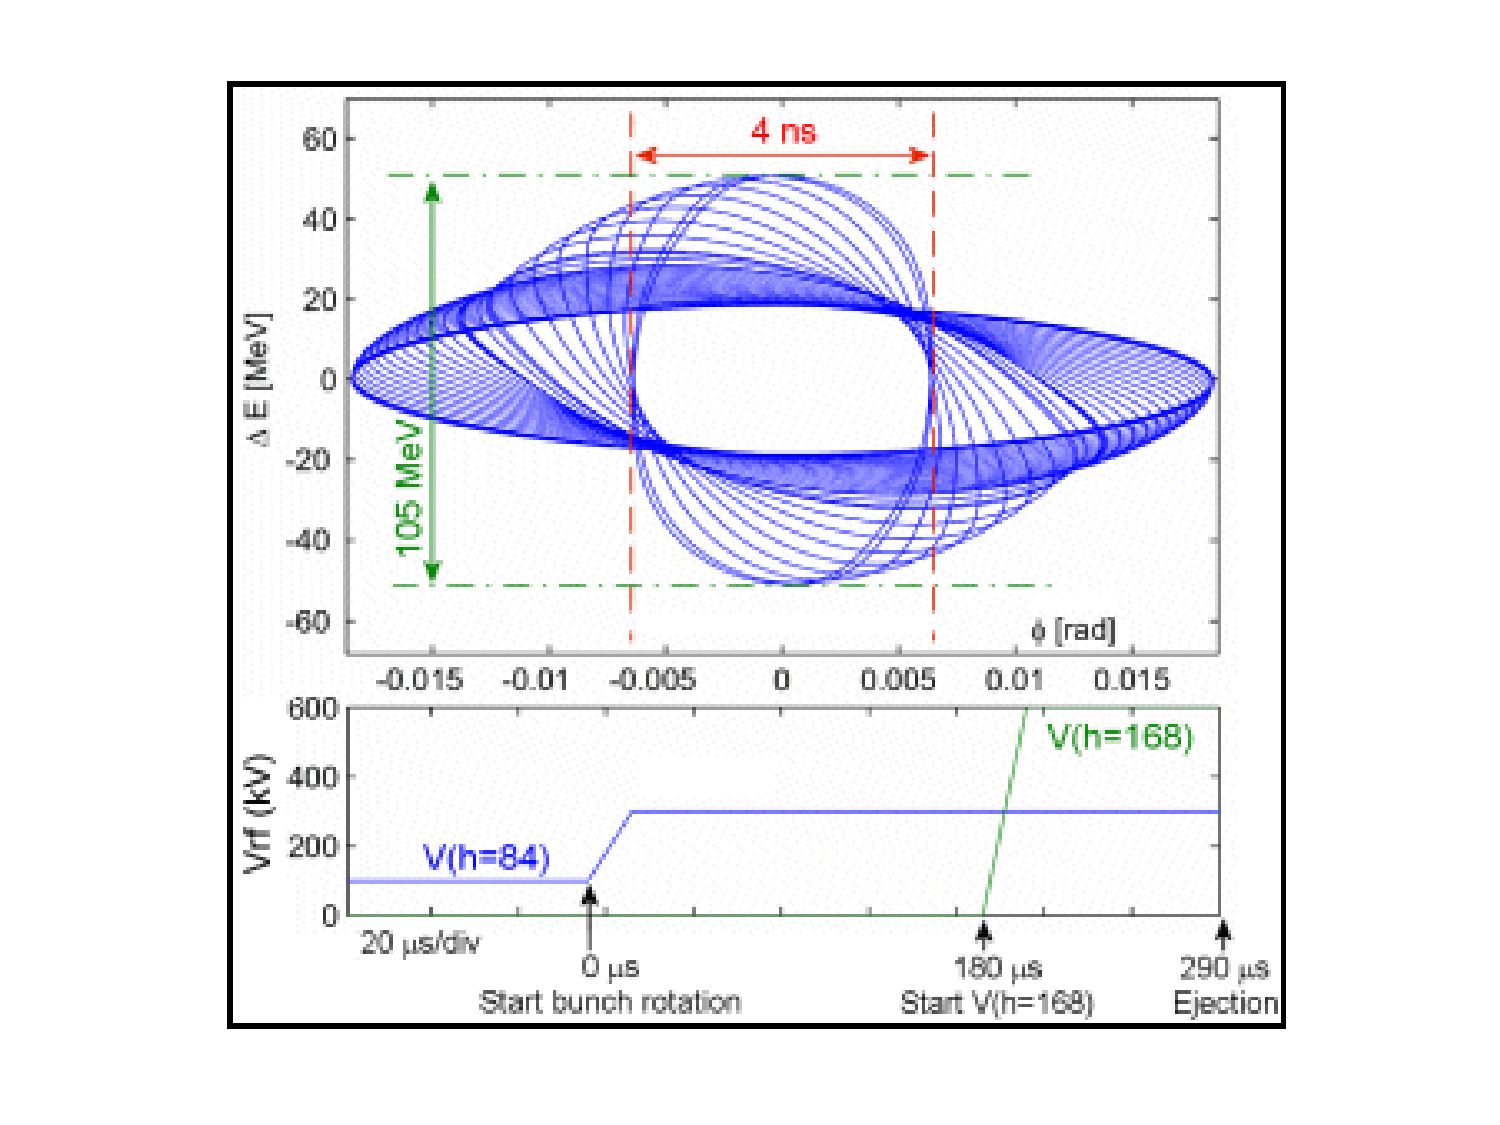
\includegraphics[width=\textwidth]{Figures/LHC_Diagrams/LHC__PS__BunchCompression.pdf}
        \caption{Rotation in phase space of the 25 \GeV proton beam,
          compressing the bunch lengths from 11 ns to 4 ns \cite{LHC:TDR_Vol3_InjectionChain_Benedikt}}\label{fig:ps_bunch_compression}
      \end{subfigure}
      \caption{Features of the PS, the third stage of
        the LHC injection chain}\label{fig:ps}
\end{figure}


\par The next stage is the Proton Synchrotron (PS), which will boost the
protons up to 25 \GeV~\cite{LHC:TDR_Vol3_InjectionChain_Benedikt}.
The layout is shown in figure \ref{fig:ps}(\subref{fig:ps_layout}).  
The ring has a circumference of 628 m, and uses 100 dipole magnets and
177 higher-order focusing magnets, to steer the beam around the ring.
Figure \ref{fig:ps}(\subref{fig:ps_dipoles}) shows a picture of one of
the dipole magnets used at the PS.  In addition to providing
acceleration up to 25 \GeV, the PS forms the basis of the bunch
structure that is eventually used in the LHC.  The $h=7$ harmonic is
used to capture the 6 bunches of protons delivered from the PS
booster, leaving a gap in the place of a seventh bunch.  The beam is
then split into three, by using three different RF cavities tuned to
the $h=7,14,21$ modes of the PS.  Figure
\ref{fig:ps}(\subref{fig:ps_split3}) shows a simulation of a proton
bunch being divided  into three over the course of 25 ms.  The $h=21$
mode is then used to accelerate the protons to from 1.4 to 25 \GeV
using the 20 MHz RF cavity.  Each bunch is then split twice,
using the $h=21,42,84$ synchrotron modes, to create 72 bunches, spaced
25 ns apart, with a 320 ns gap for the 12 unused buckets of the $h=84$
harmonic. This process is simulated in figure
\ref{fig:ps}(\subref{fig:ps_split2x2}), over the course of 125 ms. The
320 ns gap is created to account for the rise time of the  kicker
magnet, which ejects the beam out of the PS into the SPS.  The entire
splitting process is summarized in figure
\ref{fig:ps}(\subref{fig:ps_splitting}).  For the case of 50 ns bunch
spacing, the final stage of splitting is not performed, and the
$h=21,42$ modes are used to split the beam.  Finally, in order to fit
the bunches into the 200 MHz RF acceleration scheme of the SPS, the 
bunch length must be compressed from 11 ns to 4 ns.  This is achieved
by rotating the beam in the energy vs time phase space by sequential
increases in voltage to the 40 MHz $h=84$ mode, followed by an
increase to the 80 MHz $h=168$ mode.  Figure
\ref{fig:ps}(\subref{fig:ps_bunch_compression}) shows the result of
this rotation - a distortion free ellipse with a smaller 4 ns spread,
but a larger spread in the energy spectrum of the proton beam.   

\begin{figure}{h}
    \centering
    \begin{subfigure}[h]{0.45\textwidth}
        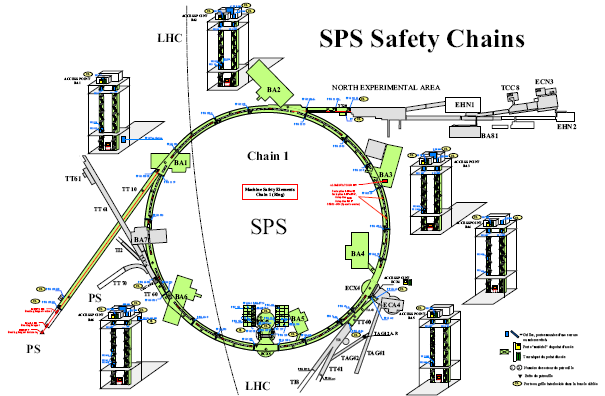
\includegraphics[width=\textwidth]{Figures/LHC_Diagrams/LHC__SPS__layout.png}
        \caption{The layout of the SPS facility \cite{LHC:LHC_sps_layout_image}}\label{fig:sps_layout}
      \end{subfigure}
      ~ %add desired spacing between images, e. g. ~, \quad, \qquad, \hfill etc.
      % (or a blank line to force the subfigure onto a new line)
    \begin{subfigure}[h]{0.45\textwidth}
        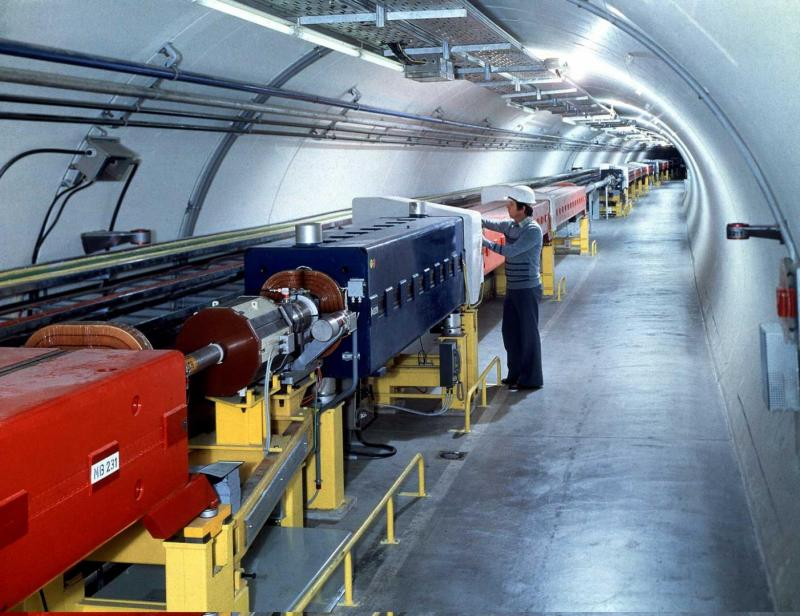
\includegraphics[width=\textwidth]{Figures/LHC_Diagrams/LHC__SPS__beamline.jpg}
        \caption{A section of dipole magnets used in the SPS \cite{LHC:LHC_sps_beamline_image}}\label{fig:sps_dipoles}
      \end{subfigure}
      ~ %add desired spacing between images, e. g. ~, \quad, \qquad, \hfill etc.
      % (or a blank line to force the subfigure onto a new line)
      \begin{subfigure}[h]{0.45\textwidth}
        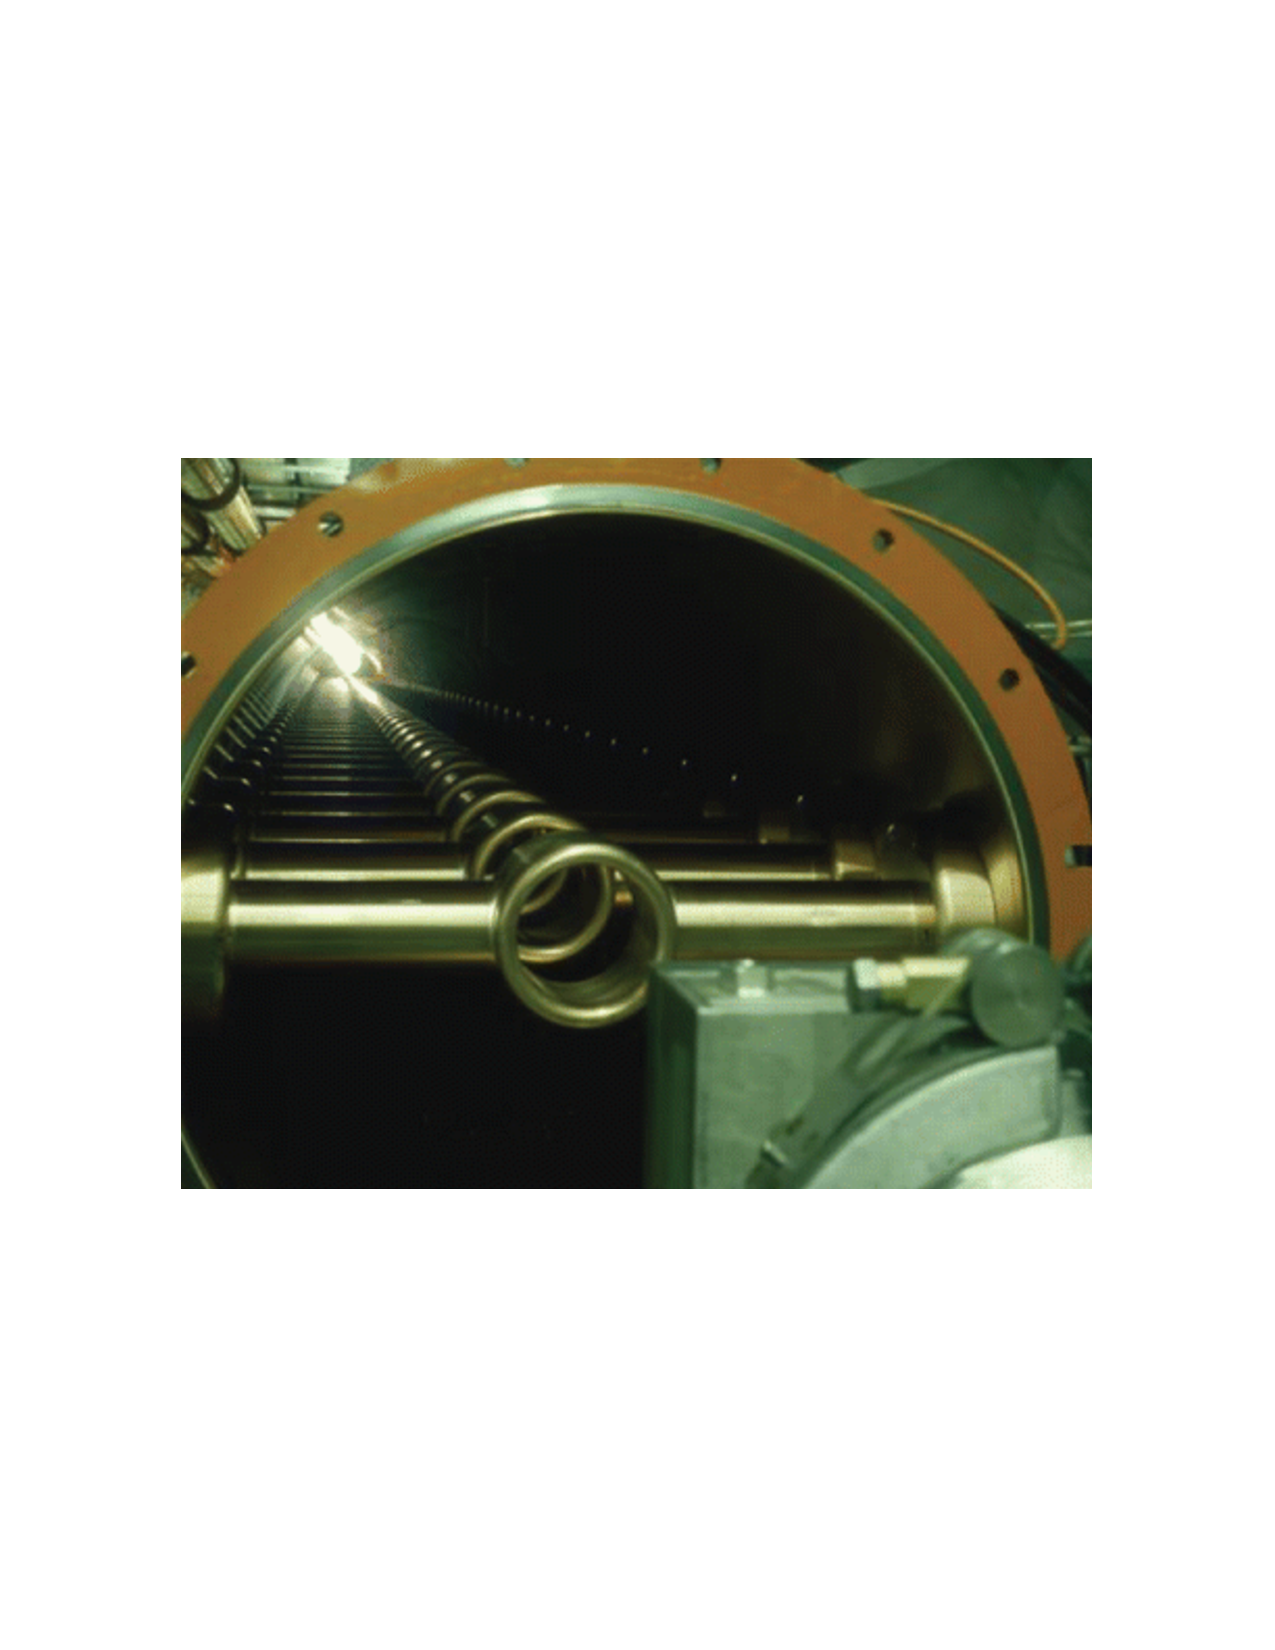
\includegraphics[width=\textwidth]{Figures/LHC_Diagrams/LHC__SPS__RFCavity_InsideView.pdf}
        \caption{The inside of the traveling wave guide structure,
          for the 200 MHz RF cavity in the SPS \cite{LHC:LHC_sps_rf_inside_image}}\label{fig:sps_rf_inside}
      \end{subfigure}
       ~ %add desired spacing between images, e. g. ~, \quad, \qquad, \hfill etc.
      % (or a blank line to force the subfigure onto a new line)
      \begin{subfigure}[h]{0.45\textwidth}
        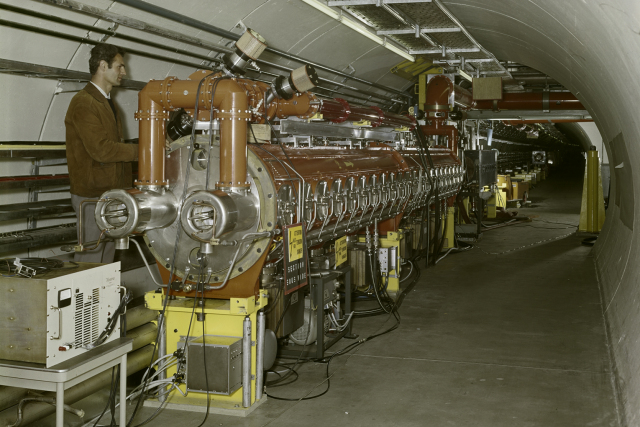
\includegraphics[width=\textwidth]{Figures/LHC_Diagrams/LHC__SPS__RFCavity_OutsideView.jpg}
        \caption{The outside of the 200 MHz RF cavity used to
          accelerate protons from 25 to 450 \GeV \cite{LHC:LHC_sps_rf_outside_image}}\label{fig:sps_rf_outside}
      \end{subfigure}
       \caption{Features of the SPS, the fourth and final stage of
        the LHC injection chain}\label{fig:sps}
\end{figure}

\par Next, the protons arrive at the Super Proton Synchrotron (SPS), where
they will be accelerated to 450 \GeV.  The SPS is the last stage of acceleration
before the protons are injected into the LHC.  The layout is show in
figure \ref{fig:sps}(\subref{fig:sps_layout}).  It has a circumference
of 7 km, and steers the proton beam with 744 dipole magnets, with 573
higher-order focusing magnets~\cite{LHC:LHC_sps_cern_website}.  Figure
\ref{fig:sps}(\subref{fig:sps_dipoles}) shows one of the dipole
magnets in the SPS tunnel.  Like all the other synchrotrons in the
injection chain, the acceleration is provided by RF cavities.  A 200
MHz system of RF cavities capture and fill the SPS by using 2-4
batches of 72 bunch proton beams from the
PS~\cite{LHC:TDR_Vol3_InjectionChain_Benedikt}.  Although the relative
change in frequency is small, the large degree of acceleration
necessitates the use of a tunable RF cavity.  The 200 MHz system has 2
sections of 4 traveling wave cavities in series, and another 2
sections of 5 cavities in series.  Figure
\ref{fig:sps}(\subref{fig:sps_rf_inside}) shows the inside of this
structure, which uses drift tubes to accelerate protons in the gaps
between tubes, with horizontally mounted bars, spaced 374
mm~\cite{LHC:LHC_SPS_200MHzRF_Dôme} apart, determining the periodicity
of the resonant RF field that builds up inside.  The outside of the
structure is shown in figure
\ref{fig:sps}(\subref{fig:sps_rf_outside}).  An additional 800 MHz
system is used to control the transverse emmitance.  It is also used
to stabilize the beam-line and prevent coupled-bunch
instabilities~\cite{LHC:TDR_Vol3_InjectionChain_Benedikt}.  

\par Finally, protons are injected into the LHC ring in one clockwise,
and another counter-clockwise rotating beams.  In order to work in the
limited space of the existing LEP tunnel, the two beams are contained
within a single mechanical and cryostat structure, with a dual-bore
design for each of the beams.  Here, each proton beam is
accelerated to their final energy of 7 \TeV, moving at 99.9999991$\%$
the speed of light, before they meet head on, producing 14 \TeV
center-of-mass collisions.  

\begin{figure}[h]
   \centering
  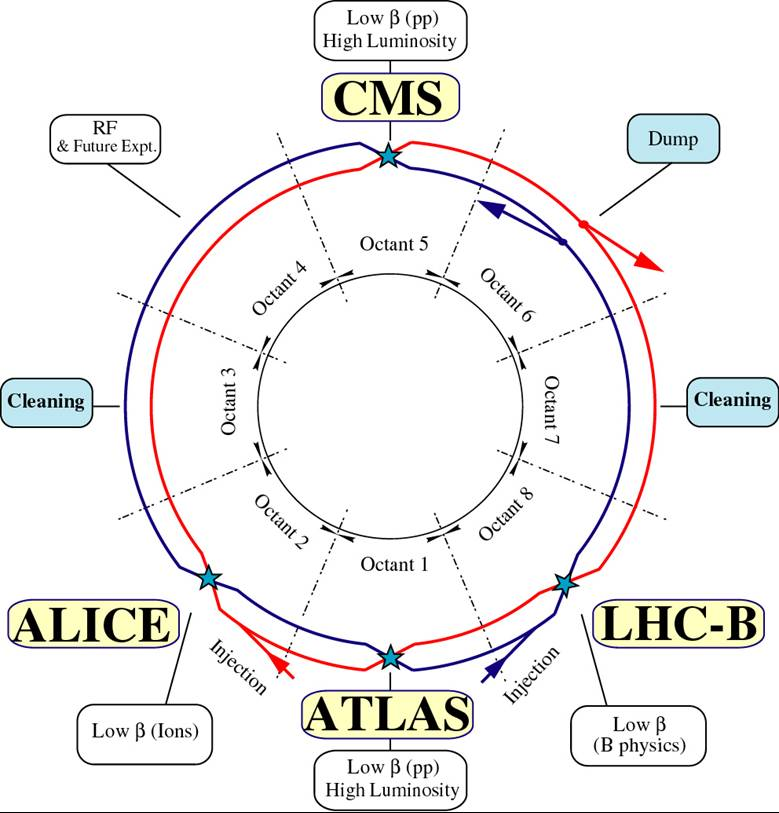
\includegraphics[width=0.8\textwidth]{Figures/LHC_Diagrams/LHC_Octant.jpg}
  \caption{The LHC ring is divided into eight octants \cite{lhc:machine_description}} \label{fig:lhc_octants}
\end{figure}

\par The LHC ring itself is divided into eight octants, with eight
straight sections that are located in front and behind each of the
eight collision points, where the beams are made to cross and
collide, as shown in figure \ref{fig:lhc_octants}.  These crossings
are known as interaction regions (IRs).  Four of these points are
currently being used by experiments.  TOTEM has detectors on either
side of the CMS experiment at one interaction region, known as point 5
(P5).  LHCf has detectors on either side of ATLAS at point 1 (P1).
MOeDAL has detectors near LHCb at point 8 (P8) and the ALICE detector
is located at point 2 (P2).  The following sections will cover the RF,
magnet, cryogen, and vacuum technologies used in the LHC ring.  


\section{LHC Magnets}
\label{lhc_magnets}

\par Several types of magnets are used in order to properly circulate
and focus the proton beam as it makes its way around the 26.7 km long
tunnel.  A complete list of all types, can be found in the technical
design report~\cite{LHC:TDR_Vol1_MainRing_Brüning}, as well as through
CERN's outreach web
resources~\cite{LHC:LHC_outreach_listOfAllMagnets}.  This section will
give an overview of the a few of the critical subsystems: the septum
and kicker magnets used for injection from the SPS, the dipole magnets
used for bending the beam around the circumference of the ring, and
the higher-order-pole magnets that are used for focusing the beam.  

\begin{figure}[h]
   \centering
  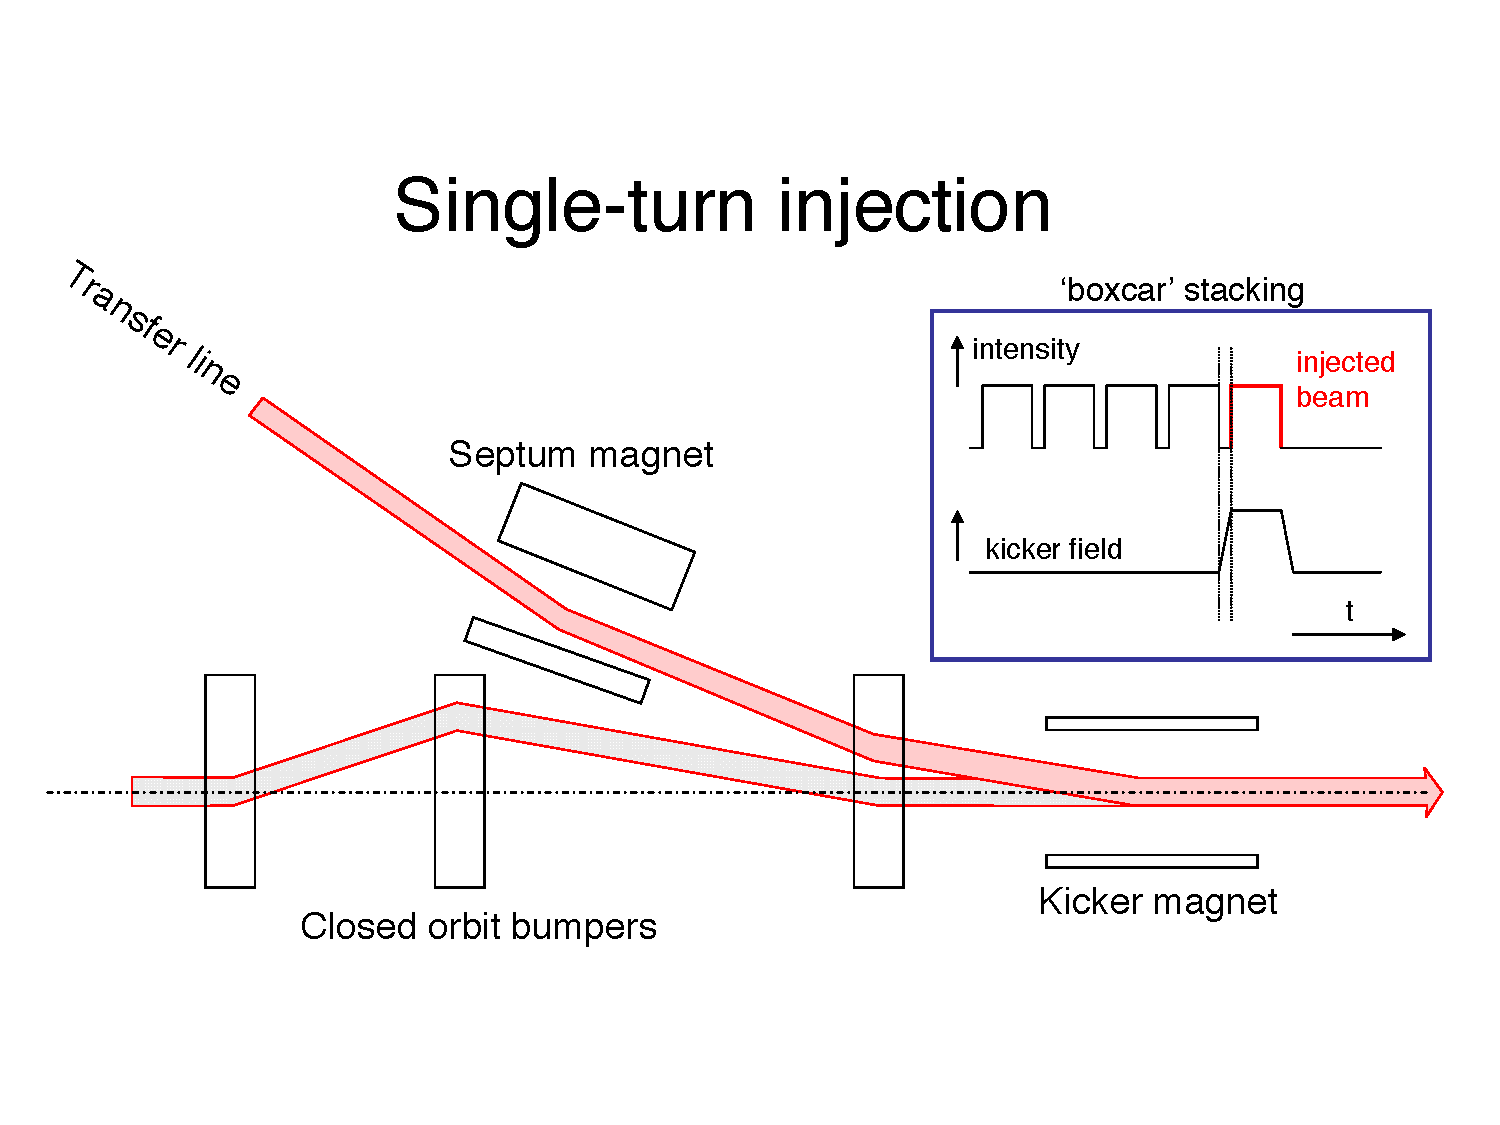
\includegraphics[width=0.8\textwidth]{Figures/LHC_Diagrams/LHC_SingleTurnInjection.pdf}
  \caption{The single turn injection scheme.  A septum magnet makes
    the initial alignment.  The kicker magnet times the injection and
    makes the final alignment.  Bumper magnets align the LHC beam with
  the injected beam \cite{LHC:LHC_kickers_Barnes}} \label{fig:lhc_singleTurnInjection}
\end{figure}

\par The injection and extraction of proton beams from one synchrotron
to another involves three types of magnets, septums, kickers, and
bumpers.  Septum magnets contain a partition, or a septum, that
provides a boundary between a high magnetic field region and a
near-zero magnetic field region and are operated in DC or a
slow-pulsed mode~\cite{LHC:LHC_septums_Barnes}.  In case of injecting
a beam of protons into a synchrotron, the target beam-pipe of the synchrotron
passes through the low-field region, so the trajectory is unaffected
by the high-field region, which bends the injection beam towards the
synchrotron aligning it horizontally, with the target beam.  The
kicker magnet, is a fast-pulsed magnet and provides the timing
selection in order to make a final vertical bend into the
synchrotron orbit, and into the correct basket of the synchrotron bunch 
train~\cite{LHC:LHC_kickers_Barnes}.  Finally, bumper magnets make
small bends to the beam and align it with the injection site.  Figure
\ref{fig:lhc_singleTurnInjection} shows a schematic for this process,
where a transfer line brings protons to a septum, which bends the beam
to a kicker, which makes the final corrections to match the
synchrotron orbit.  For extraction, the kicker magnet quickly
displaces a portion of the beam, which is steered away by the septum,
while the original beam passes through it's low-field region 
unaffected.   

\begin{figure}[h]
   \centering
  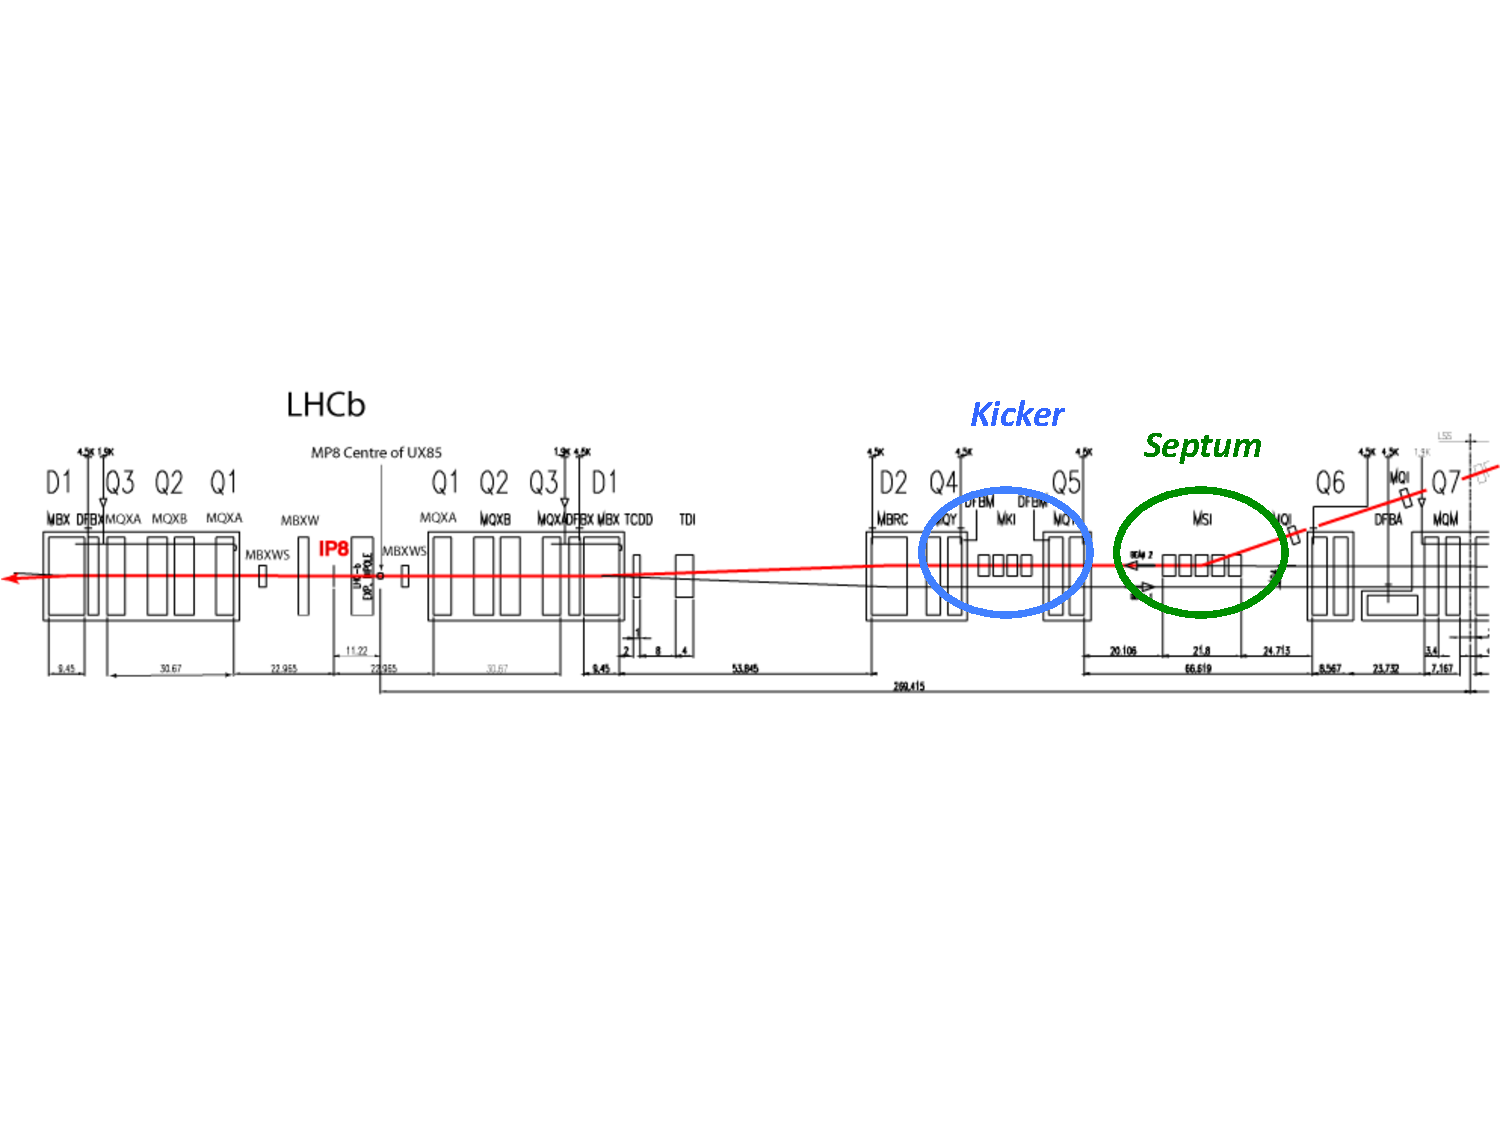
\includegraphics[width=0.8\textwidth]{Figures/LHC_Diagrams/LHC_IR8-layout.pdf}
  \caption{Layout of Interaction Region 8, where one proton beam is
    injected into the LHC ring.  A transfer line from the SPS bring a
    proton in from the right.  In green, a septum magnet aligns the
    beam horizontally with the LHC.  In blue, a kicker magnet makes
    the final vertical alignment into the LHC, and is timed to fill
    one of the 400 MHz buckets of the RF capture
    system \cite{lhc:machine_description}} \label{fig:lhc_IR8_layout}
\end{figure}

\begin{figure}[h]
   \centering
  \includegraphics[width=0.8\textwidth]{Figures/LHC_Diagrams/LHC_bunchStructure.pdf}
  \caption{The initial filling of 6 batches of protons from the PSB to
  the PS, leaves 12 empty buckets in the PS bunch structure.  The rise
time of the SPS magnet creates an additional gap in the SPS bunch
structure.  Additional gaps emerge due to the rise time of the LHC
injection and dumping kicker magnets \cite{lhc:machine_description}} \label{fig:lhc_bunchStructure}
\end{figure}

\par At the LHC, beam is injected at Interaction Regions (IR) 2 and
8~\cite{lhc:machine_description}.  Two transfer lines bring the beam
extracted from the SPS to $\sim150$ m of the LHC ring.  Five
Labertson-type septum magnets, of field strength $\sim1$ T, are used
to deflect each of the transfer line beams 12 mrad to align the
transfer beam horizontally with the LHC orbit.  Then, four $\sim0.12$T
MKI kicker magnets quickly deflect the beam 0.85 mrad to close the
orbit with the LHC ring.  Figure \ref{fig:lhc_IR8_layout} shows the
layout of the injection point at IR 8.  The green circle encloses the
septum structure, which provides the horizontal alignment, and the
blue encloses the kicker structure, which makes the final vertical
alignment and synchronizes the injection of the beam into the LHC.
The rise time for the field provided by the kicker magnets in the LHC
and SPS determine the final bunch structure of the LHC.  Figure
\ref{fig:lhc_bunchStructure} extends figure
\ref{fig:ps}(\subref{fig:ps_splitting}) showing how the rise times of
the kickers that inject, or eject beam create gaps in the bunch
structure of the LHC.  The initial filling of the PS with 6 batches of
protons from the PSB, leaves one initial bucket unused in the PS.
After the splitting of the beam into the 25 ns bunches, there 12 empty
buckets at the of the PS bunch train.  The SPS is filled with three to
four of these trains, leaving an additional 8 25 ns buckets unfilled
due to the 220 ns rise time of the SPS kicker magnet. These three to
four trains are then injected into the LHC, where there are 38 or 39
bunch gaps due to the LHC injector 0.94 $\mu$s rise time.  At the end
of a full LHC orbit, 119 buckets are left empty to allow for the rise
time of the beam dumping kicker magnet, used to remove beam from the
LHC.     

\begin{figure}{h}
    \centering
    \begin{subfigure}[h]{0.450\textwidth}
        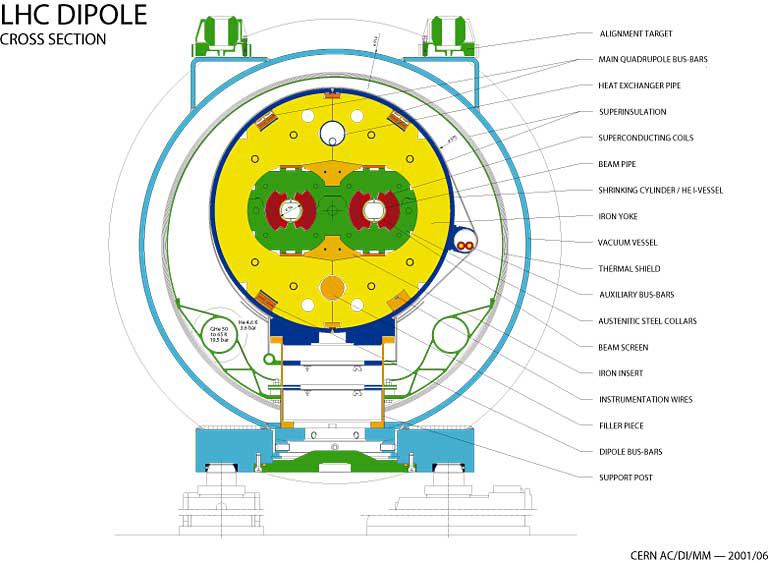
\includegraphics[width=\textwidth]{Figures/LHC_Diagrams/LHC_XSec_Dipole_Magnet__LHC-PHO-2001-187.jpg}
        \caption{Cross Section of a LHC dipole magnet \cite{lhc:machine_description}}\label{fig:lhc_dipole_xs}
      \end{subfigure}
      ~ %add desired spacing between images, e. g. ~, \quad, \qquad, \hfill etc.
      % (or a blank line to force the subfigure onto a new line)
    \begin{subfigure}[h]{0.450\textwidth}
        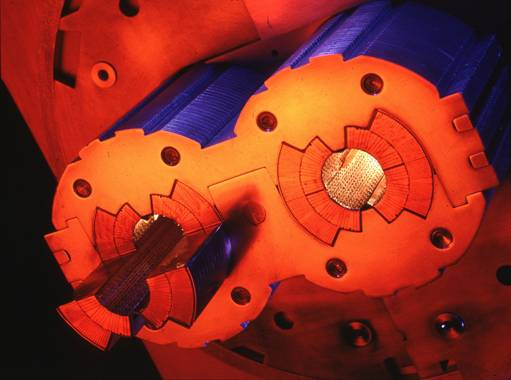
\includegraphics[width=\textwidth]{Figures/LHC_Diagrams/LHC_Dipole_CollarAndCoils.jpg}
        \caption{A close-up picture of the non-magnetic collar and
          superconducting coils of an LHC dipole magnet \cite{LHC:LHC_lhc_dipole_dual_bore_image}}\label{fig:lhc_dipole_collarAndCoils}
      \end{subfigure}
      ~ %add desired spacing between images, e. g. ~, \quad, \qquad, \hfill etc.
      % (or a blank line to force the subfigure onto a new line)
      \begin{subfigure}[h]{0.450\textwidth}
        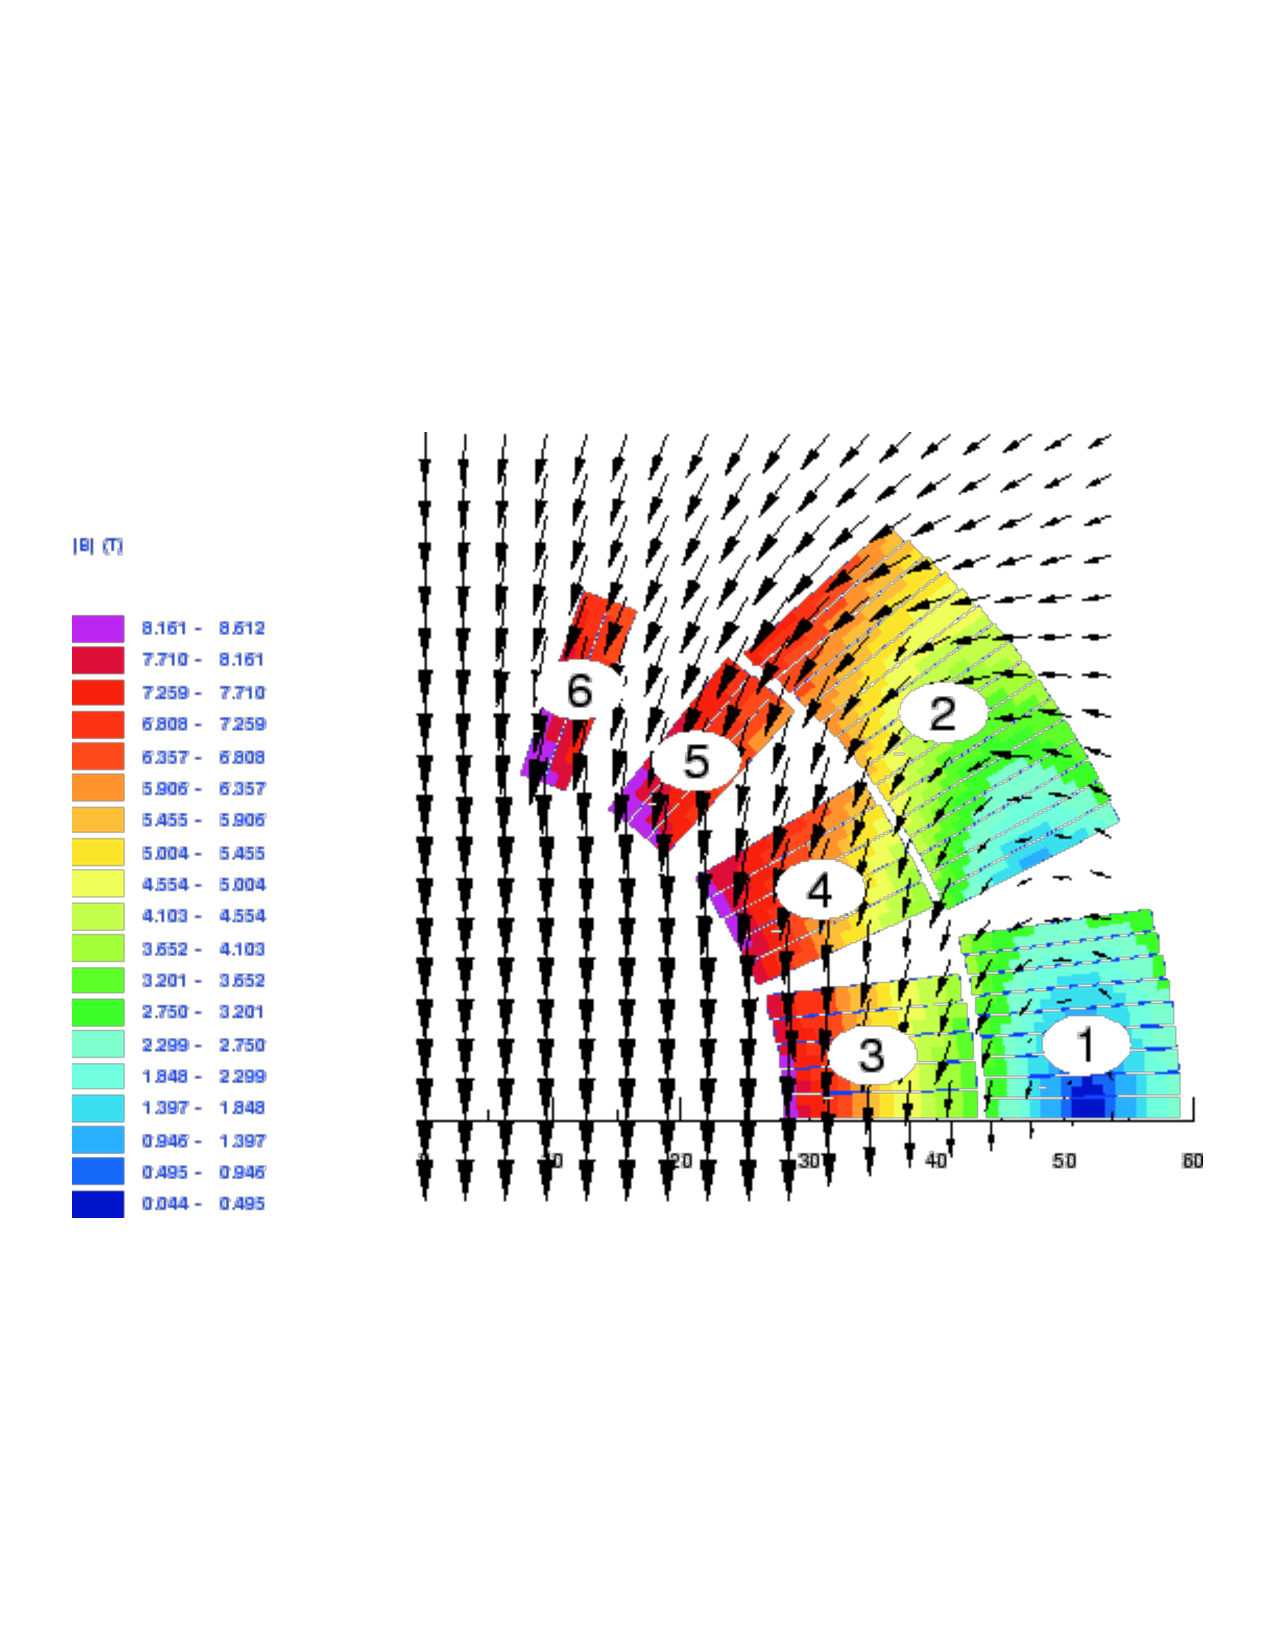
\includegraphics[width=\textwidth]{Figures/LHC_Diagrams/LHC_Dipole_Field.pdf}
        \caption{A simulation of the homogenous, vertical magnetic field lines of the
          dipole \cite{LHC:LHC_lhc_dipole_field_image}. }\label{fig:lhc_dipole_field}
      \end{subfigure}
       ~ %add desired spacing between images, e. g. ~, \quad, \qquad, \hfill etc.
      % (or a blank line to force the subfigure onto a new line)
      \begin{subfigure}[h]{0.450\textwidth}
        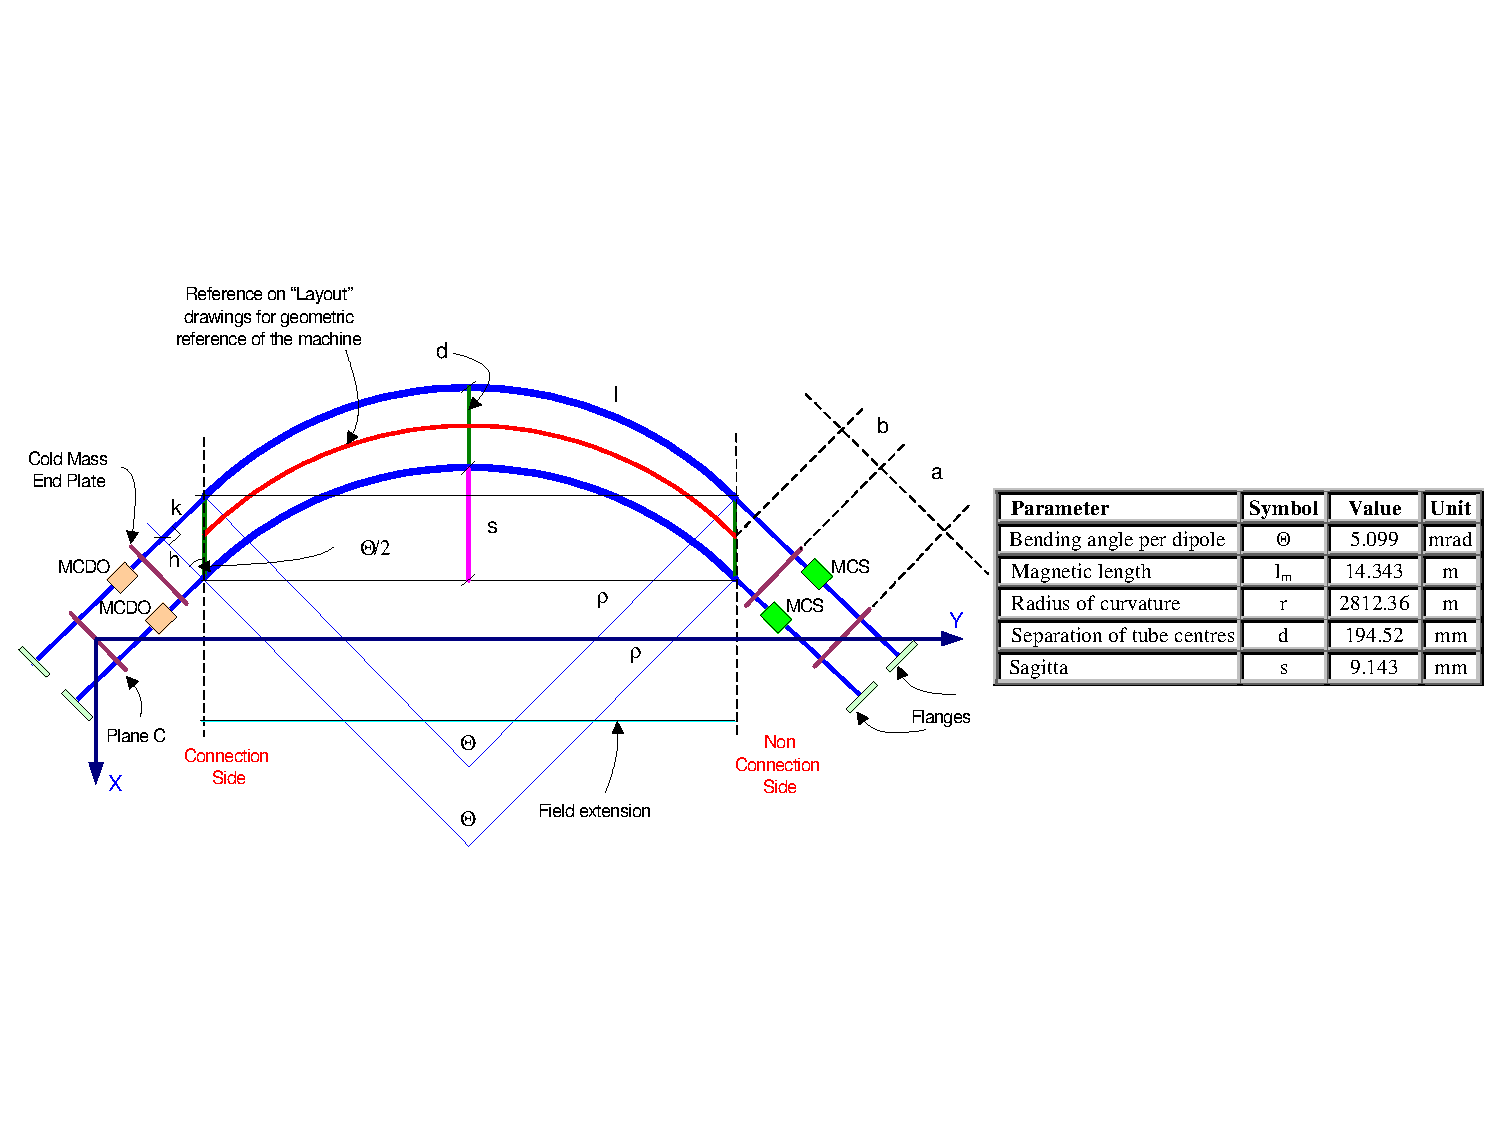
\includegraphics[width=\textwidth]{Figures/LHC_Diagrams/LHC_Dipole_ExageratedCurvature.pdf}
        \caption{A diagram showing the exaggerated curvature of a
          dipole magnet, with measurements for some of it's most
          important features \cite{LHC:LHC_lhc_dipole_Beauquis}. }\label{fig:lhc_dipole_curvature}
      \end{subfigure}
      \begin{subfigure}[h]{0.450\textwidth}
        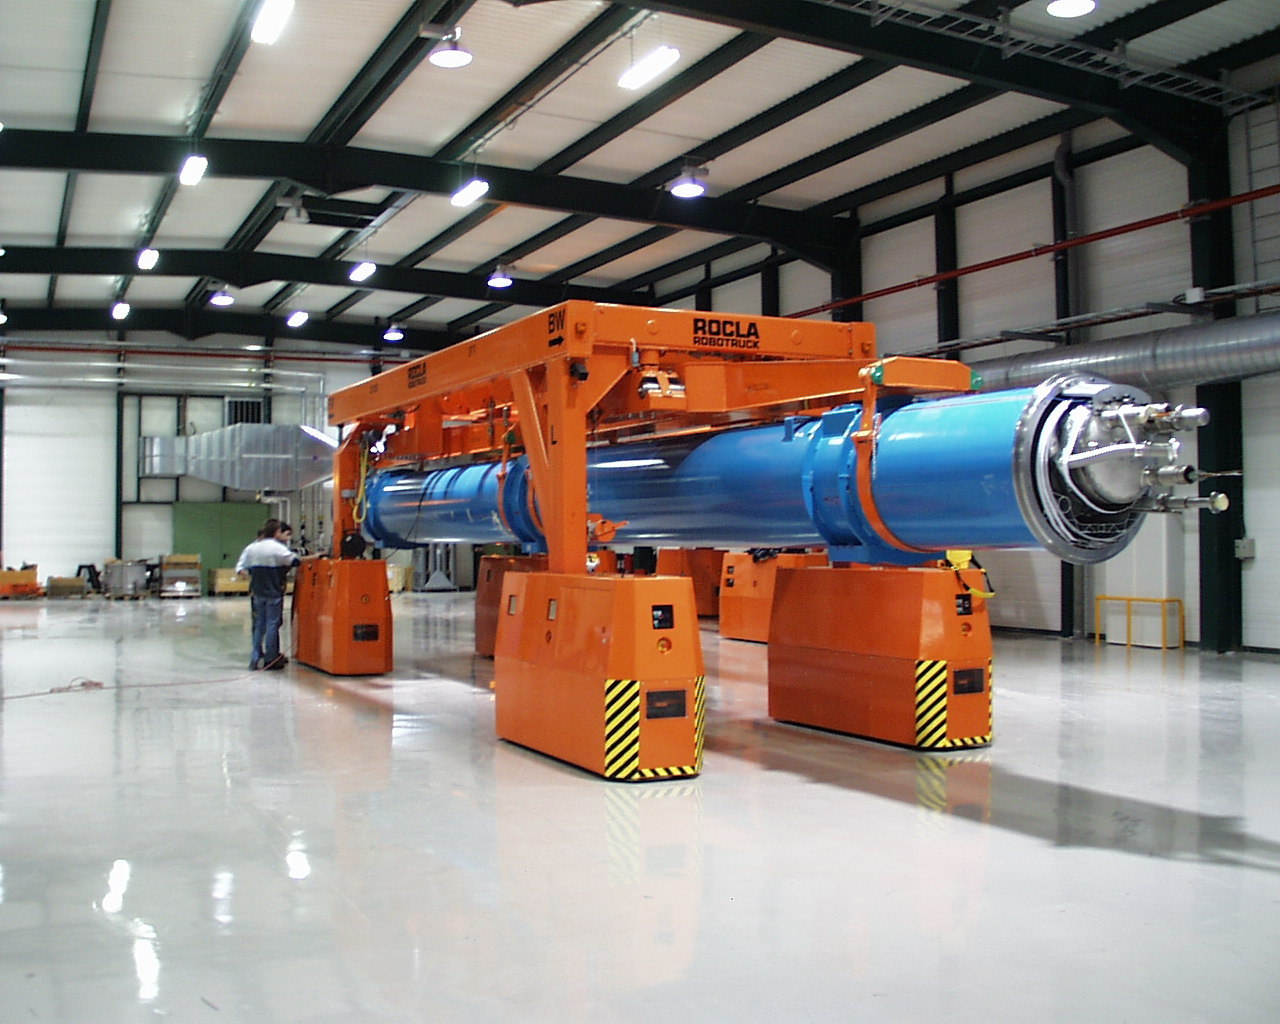
\includegraphics[width=\textwidth]{Figures/LHC_Diagrams/LHC_Dipole_transp-2001-001_05.jpg}
        \caption{A $\sim$15 m long dipole magnet, in a staging area at
        CERN, awaiting installation \cite{LHC:LHC_lhc_dipole_image}}\label{fig:lhc_dipole_staging}
      \end{subfigure}
       \caption{Features of the dipole magnets used in the LHC}\label{fig:lhc_dipole}
\end{figure}

\par Once the beam is injected, the curved path around the
circumference of the LHC is maintained via 1232 superconducting dipole
magnets.  The superconducting material niobium-titanium, NbTi, is
cooled to 1.9 K in order to produce the 8.33 T field.  Figure
\ref{fig:lhc_dipole}(\subref{fig:lhc_dipole_xs}) shows a cross-section
view of one of the LHC dipoles.  The dual-bore design of the beam-pipe
is enclosed by an iron yoke, that serves as the cold mass to maintain
the superconducting temperature, and provides a 195 mm gap between
each beam.  A close up picture of the non-magnetic collar and
superconducting coils are shown in figure
\ref{fig:lhc_dipole}(\subref{fig:lhc_dipole_collarAndCoils}).  A
simulation  of the magnet in figure
\ref{fig:lhc_dipole}(\subref{fig:lhc_dipole_field}) shows the
homogenous, vertical magnetic field produced in the center of the
coil.  Diagram \ref{fig:lhc_dipole}(\subref{fig:lhc_dipole_curvature})
shows an exaggerated view of the 2812 m radius curvature of each
dipole. However, since each dipole is only $\sim14$ m in length, this
curvature is hardly noticeable, as shown in a photo of an actual
dipole magnet in a staging area at CERN, awaiting installation in
figure \ref{fig:lhc_dipole}(\subref{fig:lhc_dipole_staging}).   

\begin{figure}{h}
    \centering
    \begin{subfigure}[h]{0.450\textwidth}
        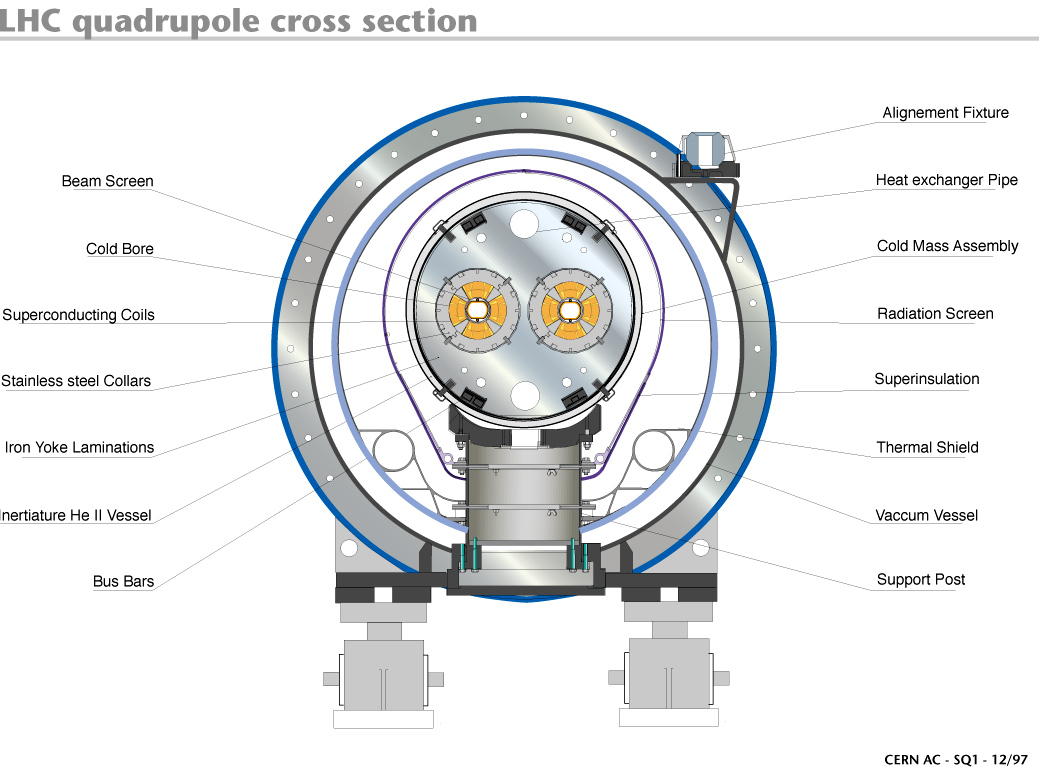
\includegraphics[width=\textwidth]{Figures/LHC_Diagrams/LHC_Quardupole_Schematic-1998-312.jpg}
        \caption{Cross Section of a LHC quadrupole magnet \cite{LHC:LHC_lhc_quadrupole_schematic_image}}\label{fig:lhc_quadrupole_xs}
      \end{subfigure}
      ~ %add desired spacing between images, e. g. ~, \quad, \qquad, \hfill etc.
      % (or a blank line to force the subfigure onto a new line)
    \begin{subfigure}[h]{0.450\textwidth}
        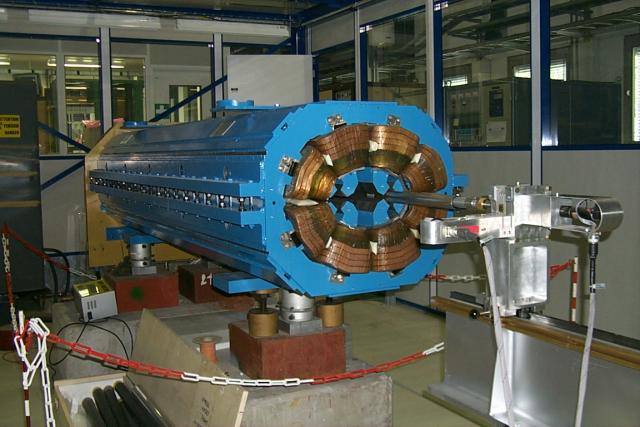
\includegraphics[width=\textwidth]{Figures/LHC_Diagrams/LHC_Quadrupole_TwinMagnets_Staged.jpg}
        \caption{A dual-bore quadrupole magnet, in a staging area
          prior to installation \cite{LHC:LHC_lhc_quadrupole_staged_image}}\label{fig:lhc_quadrupole_staged}
      \end{subfigure}
      ~ %add desired spacing between images, e. g. ~, \quad, \qquad, \hfill etc.
      % (or a blank line to force the subfigure onto a new line)
      \begin{subfigure}[h]{0.450\textwidth}
        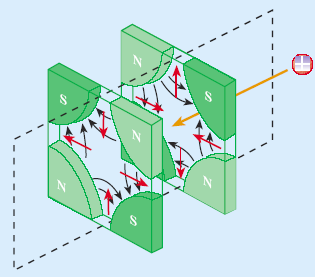
\includegraphics[width=\textwidth]{Figures/LHC_Diagrams/LHC_Quadrupole_Focusing.png}
        \caption{A quadrupole magnet can provide focusing either in
          the horizontal or vertical direction \cite{LHC:LHC_lhc_quadrupole_focusing_schematic_image}}\label{fig:lhc_quadrupole_field}
      \end{subfigure}
       ~ %add desired spacing between images, e. g. ~, \quad, \qquad, \hfill etc.
      % (or a blank line to force the subfigure onto a new line)
      \begin{subfigure}[h]{0.450\textwidth}
        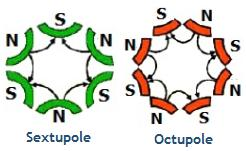
\includegraphics[width=\textwidth]{Figures/LHC_Diagrams/LHC_MultipoleFields.jpg}
        \caption{Multipole fields from a sextupole and an octupole
          magnet \cite{LHC:LHC_lhc_multipole_focusing_schematic_image}}\label{fig:lhc_multipole_field}
      \end{subfigure}
      \begin{subfigure}[h]{0.450\textwidth}
        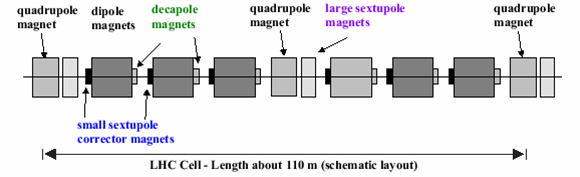
\includegraphics[width=\textwidth]{Figures/LHC_Diagrams/LHC_MagneticCell.png}
        \caption{A typical 110m long magnetic cell at the LHC featuring
        several types of multipole magnets \cite{LHC:LHC_lhc_magnetic_cell_schematic_image}}\label{fig:lhc_magnetic_cell}
      \end{subfigure}
      ~ %add desired spacing between images, e. g. ~, \quad, \qquad, \hfill etc.
      % (or a blank line to force the subfigure onto a new line)
      \begin{subfigure}[h]{0.450\textwidth}
        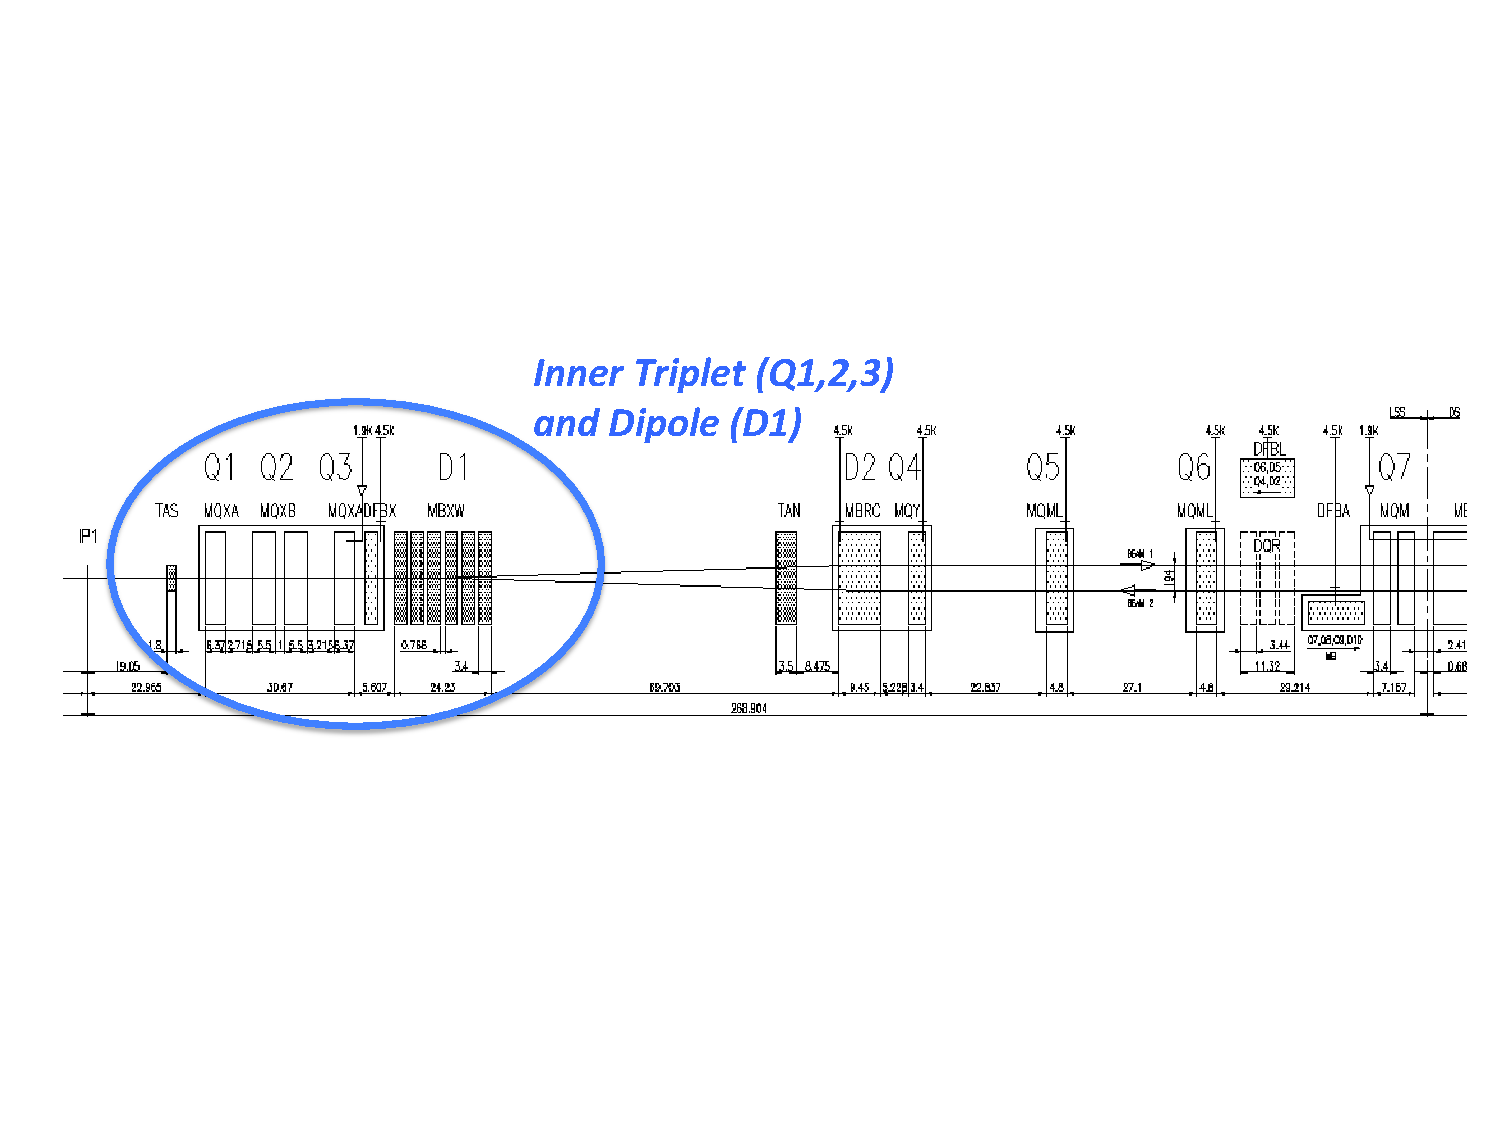
\includegraphics[width=\textwidth]{Figures/LHC_Diagrams/LHC_InnerTriplet.pdf}
        \caption{Schematic of the Inner triplet structure that brings
          the two separate beams together in the interaction region \cite{lhc:machine_description}}\label{fig:lhc_inner_triplet}
      \end{subfigure}
      ~ %add desired spacing between images, e. g. ~, \quad, \qquad, \hfill etc.
      % (or a blank line to force the subfigure onto a new line)
      \begin{subfigure}[h]{0.450\textwidth}
        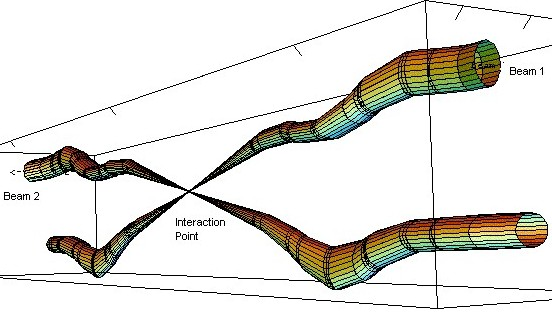
\includegraphics[width=\textwidth]{Figures/LHC_Diagrams/LHC_InteractionRegion.jpg}
        \caption{A simulation of two beams being squeezed together by
          the inner triplet \cite{LHC:LHC_lhc_IR_schematic_image}}\label{fig:lhc_beam_squeeze}
      \end{subfigure}
       \caption{Features of the dipole magnets used in the LHC}\label{fig:lhc_multipole}
\end{figure}


\par Quadrupole, sextupole, octupole, and other multipole magnets are
used to focus a single beam, as well as squeeze the two beams
together.  There are 392 quadrupole magnets
on the LHC ring, each controlling the height and width of the beam.
Figure \ref{fig:lhc_multipole}(\subref{fig:lhc_quadrupole_xs}) shows a
schematic of a dual-bore quadrupole magnet, and figure
\ref{fig:lhc_multipole}(\subref{fig:lhc_quadrupole_staged}) shows an
actual quadrupole in a staging area before  installation.  Quadrupole
magnets use four sets of coils to create a magnetic field that either
squeezes the beam horizonally or vertically, as shown in figure
\ref{fig:lhc_multipole}(\subref{fig:lhc_quadrupole_field}). Finer
corrections to the beam shape are made with the multipole magnets,
since they are able to compress the beam from more than two axes.
Figure \ref{fig:lhc_multipole}(\subref{fig:lhc_multipole_field})
shows the fields lines of a sextupole and  octupole magnet.  A typical
cell of magnets, 110 m long, in the LHC octant is shown in a diagram
in figure \ref{fig:lhc_multipole}(\subref{fig:lhc_magnetic_cell}), where the dipole, 
quadrupole and higher order magnets work in series to confine the
protons to the LHC ring.  Finally, a set of single bore magnets, known
as an inner triplet, bring the two beams together into an interaction
region.  Figure
\ref{fig:lhc_multipole}(\subref{fig:lhc_inner_triplet}) shows the
arrangement of magnets that squeeze the beam together, while figure
\ref{fig:lhc_multipole}(\subref{fig:lhc_beam_squeeze}) shows a
simulation of the beams being brought together to collide in the
interaction region.  


\section{LHC RF Technology}
\label{lhc_rf_overview}

\begin{figure}{h}
    \centering
    \begin{subfigure}[h]{0.450\textwidth}
        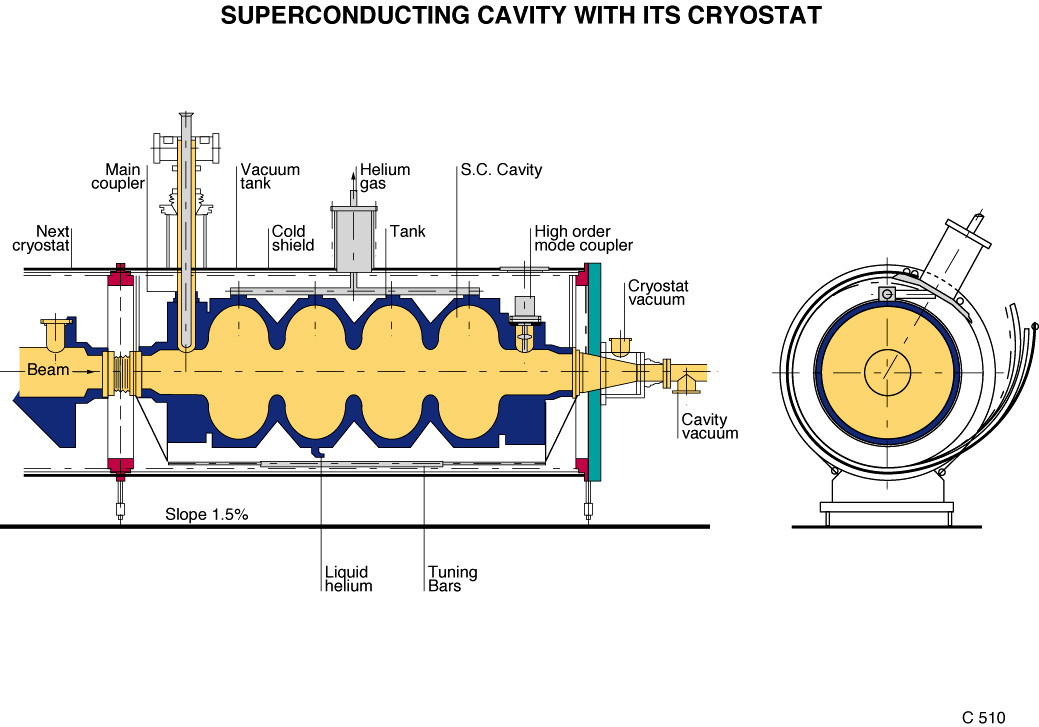
\includegraphics[width=\textwidth]{Figures/LHC_Diagrams/LHC_RFCavity_Schematic-1994-006.jpg}
        \caption{Cross section of a LHC superconducting Radio
          Frequency cavities, which accelerates the beam by imparting
          275 kW of power through a 400 MHz, 16 MV electric field
          resonating in the cavity \cite{Jean-Luc:841461}.}\label{fig:lhc_rf_xs}
      \end{subfigure}
      ~ %add desired spacing between images, e. g. ~, \quad, \qquad, \hfill etc.
      % (or a blank line to force the subfigure onto a new line)
    \begin{subfigure}[h]{0.450\textwidth}
        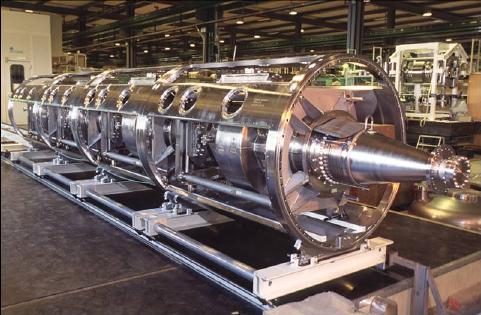
\includegraphics[width=\textwidth]{Figures/LHC_Diagrams/LHC_RFCavity_Staged.jpg}
        \caption{A picture of a four chamber RF cavity in a staging
          area, prior to installation \cite{LHC:LHC_lhc_rfcav_staged_image}}\label{fig:lhc_rf_staged}
      \end{subfigure}
      ~ %add desired spacing between images, e. g. ~, \quad, \qquad, \hfill etc.
      % (or a blank line to force the subfigure onto a new line)
      \begin{subfigure}[h]{0.450\textwidth}
        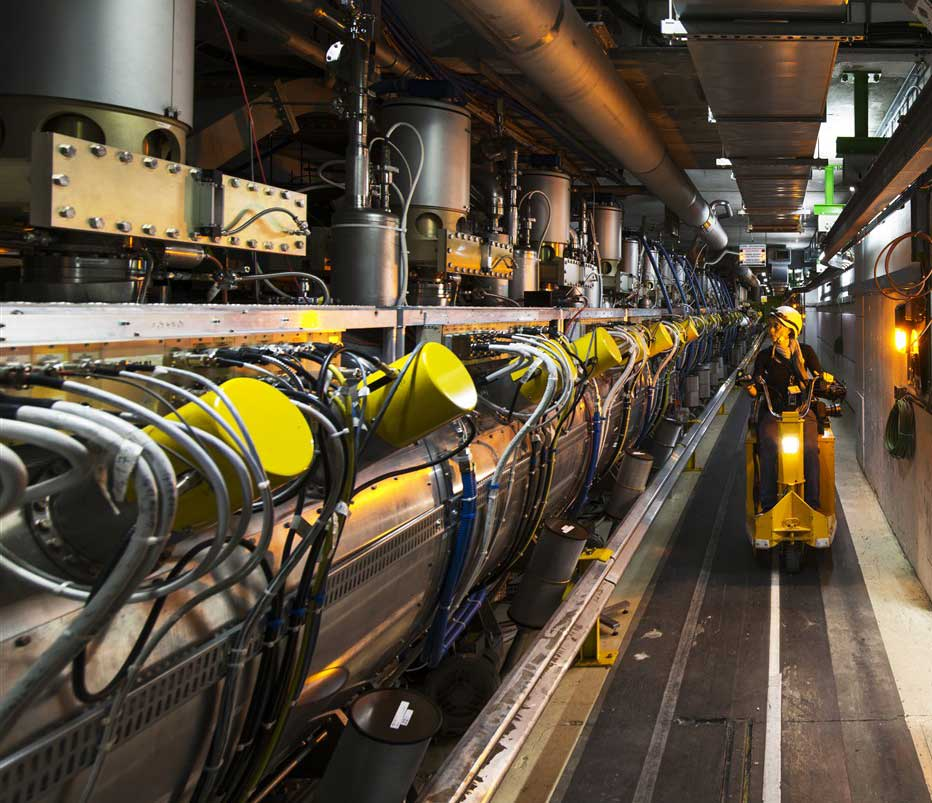
\includegraphics[width=\textwidth]{Figures/LHC_Diagrams/LHC_RFCavity_Installed.jpg}
        \caption{The four chamber RF cavity installed at Point 4 of
          the LHC \cite{LHC:LHC_lhc_rfcav_installed_image}}\label{fig:lhc_rf_at_p4}
      \end{subfigure}
      \caption{Features of the 400 MHz superconducting RF system used in the LHC}\label{fig:lhc_rf}
\end{figure}

\par The LHC uses a 400 MHz superconducting RF cavity system to
capture and accelerate the beam from 450 \GeV to 7
\TeV~\cite{lhc:machine_description}.  Two independent system are used
to provide 8 MV of RF voltage at injection at 16 MV during equilibrium
at 7 \TeV and deliver 275 kW of power to each beam.  This is provided
by 16 niobium sputtered cavities, housed in 4.5 K refrigeration units,
known as cryo-modules, at Point 4 of the LHC octant.  The
superconducting material covering the inside of the cavity has
near-zero resistivity, which dissipates much less power and has a much
narrower resonance width, or Q-factor, than a cavity made from
normally conducting material. Figure
\ref{fig:lhc_rf}(\subref{fig:lhc_rf_xs}) shows a schematic of a four
cavity cryo-module.  The beam pipe passes through the center of each
chamber and longitudinal (left to right in the diagram) electric
fields accelerate the protons each time they circulate the LHC
ring. Figure \ref{fig:lhc_rf}(\subref{fig:lhc_rf_staged}) shows an
actual four cavity module in a staging area prior to installation.  In
this picture, the resonance cavities are concealed underneath the
cylindrical housing of the vacuum tank and cryostat.  Figure
\ref{fig:lhc_rf}(\subref{fig:lhc_rf_at_p4}) is a picture of the
module installed at Point 4.  The thin cylindrical structures
extending off the top is the LHe intake valve and quench system.  The
thicker cylindrical structures are the waveguides that couple the
cavities to the source of the electric field, the klystrons.   

\begin{figure}[h]
   \centering
  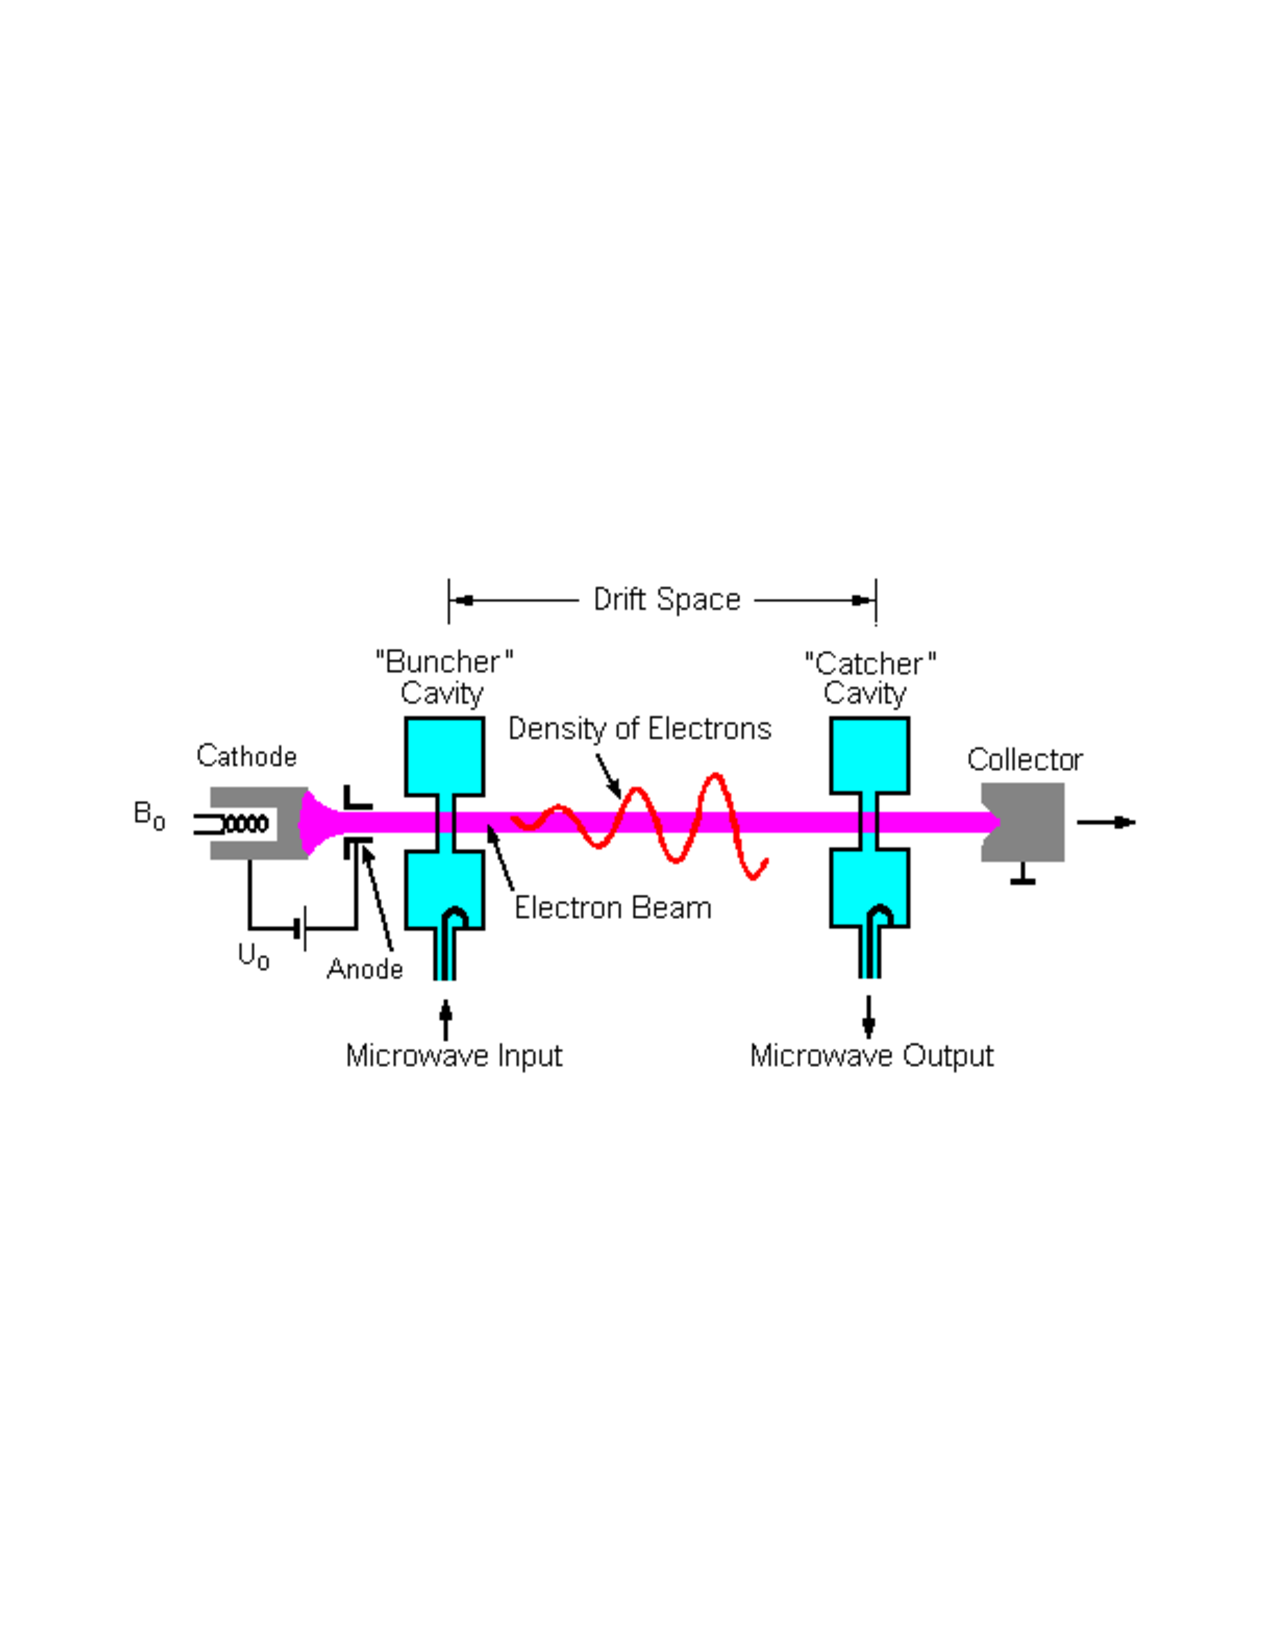
\includegraphics[width=0.8\textwidth]{Figures/LHC_Diagrams/LHC_KlystronBasic.pdf}
  \caption{A klystron uses a weak RF signal coupled to a resonance
    cavity to bunch an electron beam, which in turn creates an
    amplified RF signal as it passes through a second resonance cavity
    tuned to the same frequency \cite{LHC:LHC_klyston_basic}.} \label{fig:lhc_klystron_operation}
\end{figure}

\par A Klystron is the source of RF power that builds up as a
resonance in the cavities that accelerate the protons.  Figure
\ref{fig:lhc_klystron_operation} shows a diagram of the basic
operating principle.  The device uses an anode to accelerate the
thermionic emission of electrons off of a cathode material into one or
more bunching cavities tuned to the frequency the device is designed
to produce.  This cavity is driven with a weak RF source, that groups
electrons into bunches.  Just as discussed for protons earlier, when
electrons arrive at the entrance of the cavity at just the right time,
it will experience the zero-point of the oscillation of the resonating
electric field.  If it arrives early or late, it is accelerated or
decelerated and thus bringing it closer to its neighbors, and
increasing the density of the beam.  After passing through multiple
chambers, the tightly bunched electrons enter a catcher cavity tuned
to the same resonance frequency.  As the electrons pass through at
this resonance frequency, standing electric waves are excited and
quickly build up in the catcher cavity.  The electron beam is thus
used to amplify the original RF signal in the catcher cavity, which is
then transported via waveguide to power the RF cavity used to
accelerate the proton beam-line.  

\begin{figure}[h]
   \centering
  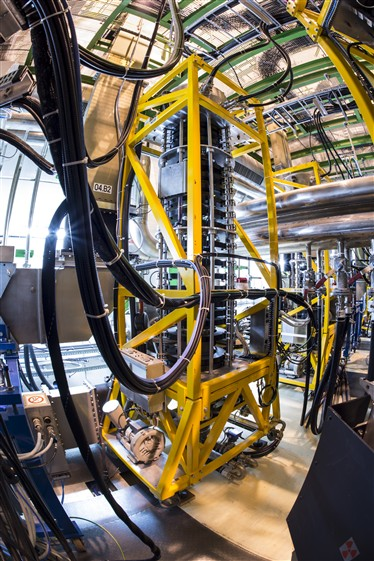
\includegraphics[width=0.6\textwidth]{Figures/LHC_Diagrams/LHC_Klystron_Installed.jpg}
  \caption{One of sixteen 300 kW, 400 MHz klystrons that power the
    superconducting RF cavities that accelerate the proton beam \cite{LHC:LHC_klyston_installed}.} \label{fig:lhc_klystron}
\end{figure}

\par At the LHC, 16 400 MHz, 300 kW klystrons, work together to provide 4800 kW
of power to the superconducting RF
cavities~\cite{lhc:machine_description}.  They are also located at
Point 4, in the UX45 service cavern adjacent to the RF cavities, about
6 m below the beam-line.  An average of 22 m of waveguide is used to
transport the power generated by the klystrons to the RF cavities.
Figure \ref{fig:lhc_klystron} shows a klystron installed at the LHC, and like most modern
klystrons, it also utilizes a multi-bunching chamber design.

\section{The LHC Cryogen System}
\label{lhc_cryogen_overview}

\begin{figure}[h]
   \centering
  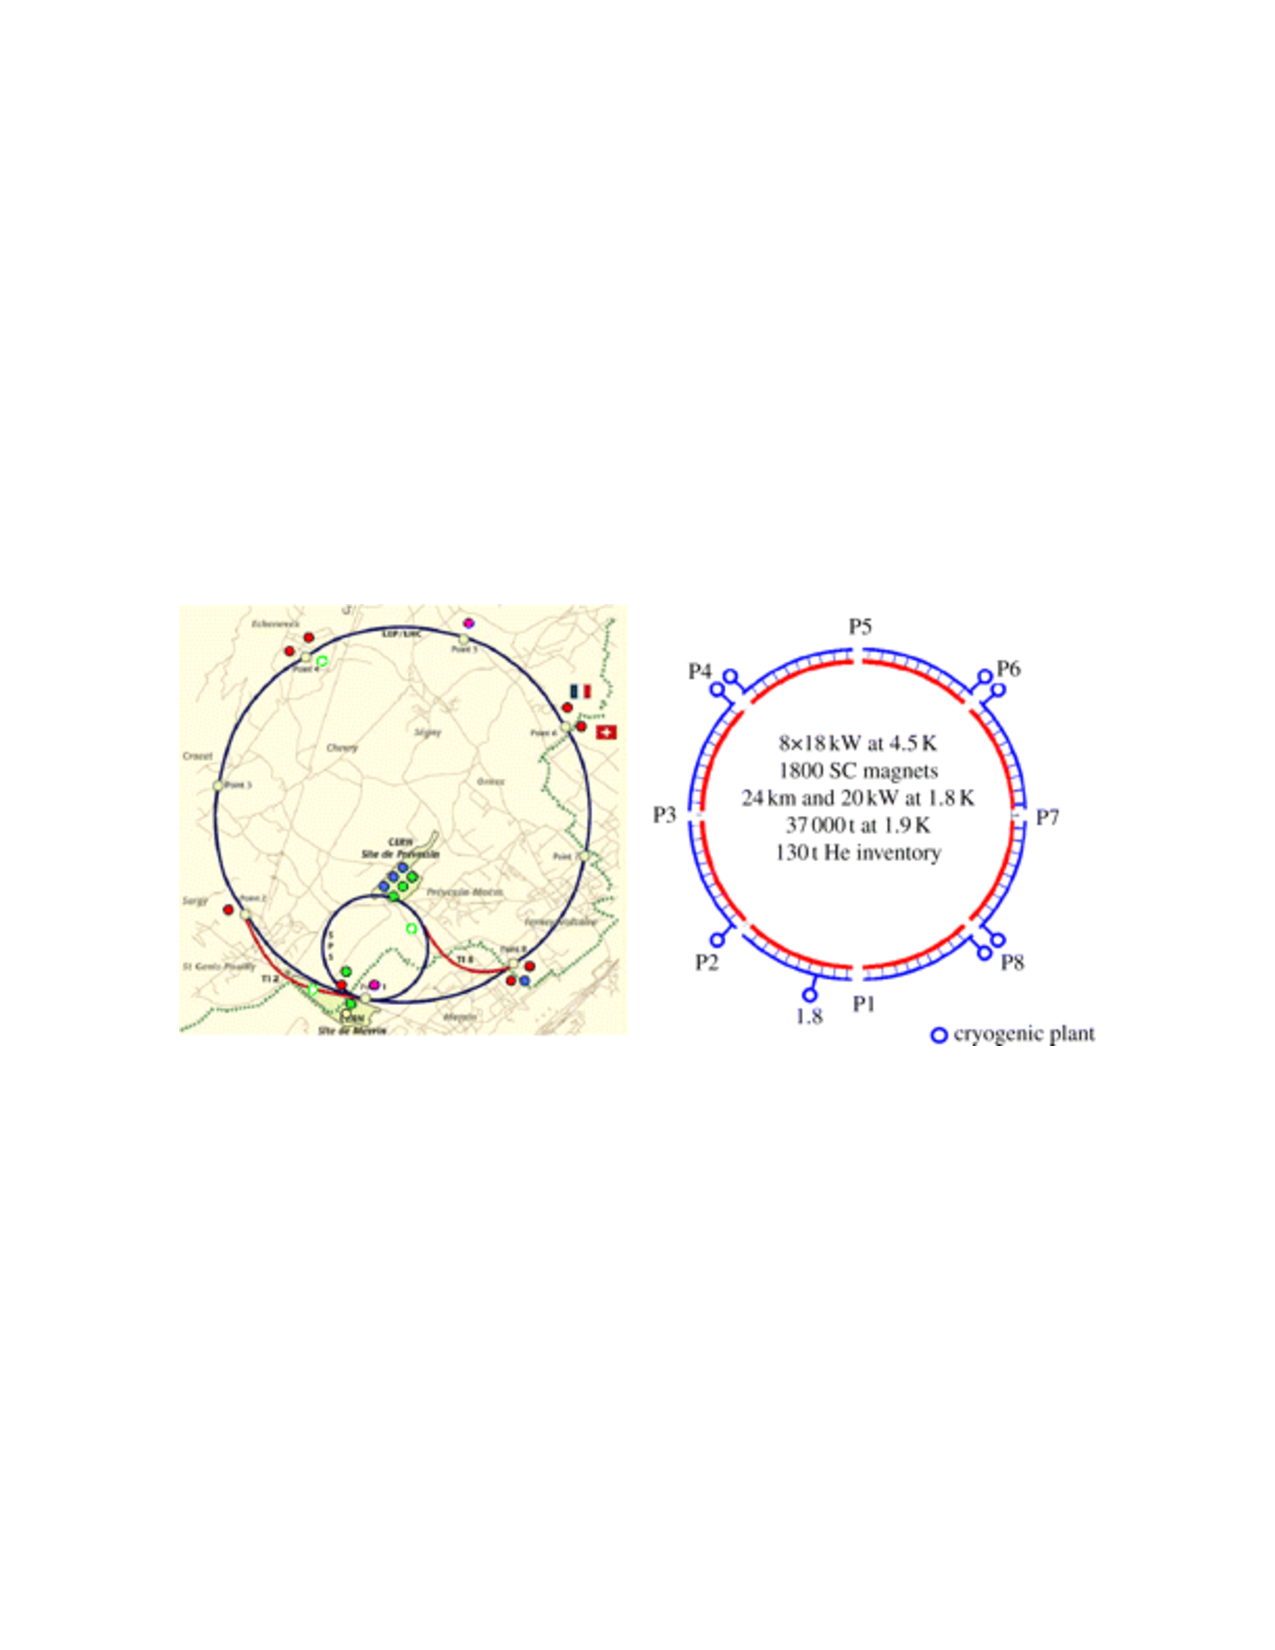
\includegraphics[width=0.6\textwidth]{Figures/LHC_Diagrams/LHC_CoolingPlants.pdf}
  \caption{Layout of the five cryogenic islands, which are home to the
  eight facilities that provide liquid helium to the LHC \cite{LHC:LHC_lhc_cryogen_islands_layout_image}} \label{fig:lhc_cryogenic_islands}
\end{figure}

\par The LHC is the largest cryogenic system in the
world~\cite{LHC:LHC_lhc_cryogen_cernWebsite}, as its operating
temperature is 1.8 K, in order to produce the high-magnetic fields
needed by the dipole magnets.  Additionally, the acceleration
mechanism, the RF cavities, are also superconducting, and must be 
cooled to 4.5 K.  Over 120 tons of Helium are used as the cryogenic
medium, since once it is cooled below 2.17 K, it becomes a superfluid,
a phase of matter with a high thermal conductivity, making it ideal
for refrigeration.  Cryogenic and auxiliary equipment are
concentrated into 5 "cryogenic islands" at Points 1,2,4,6, and
8~\cite{lhc:machine_description}.  As shown in figure
\ref{fig:lhc_cryogenic_islands}, Points 4,6, and 8 house two facilities
each, making a total of eight, one for each octant of the LHC arc. 

\begin{figure}{h}
    \centering
    \begin{subfigure}[h]{0.450\textwidth}
        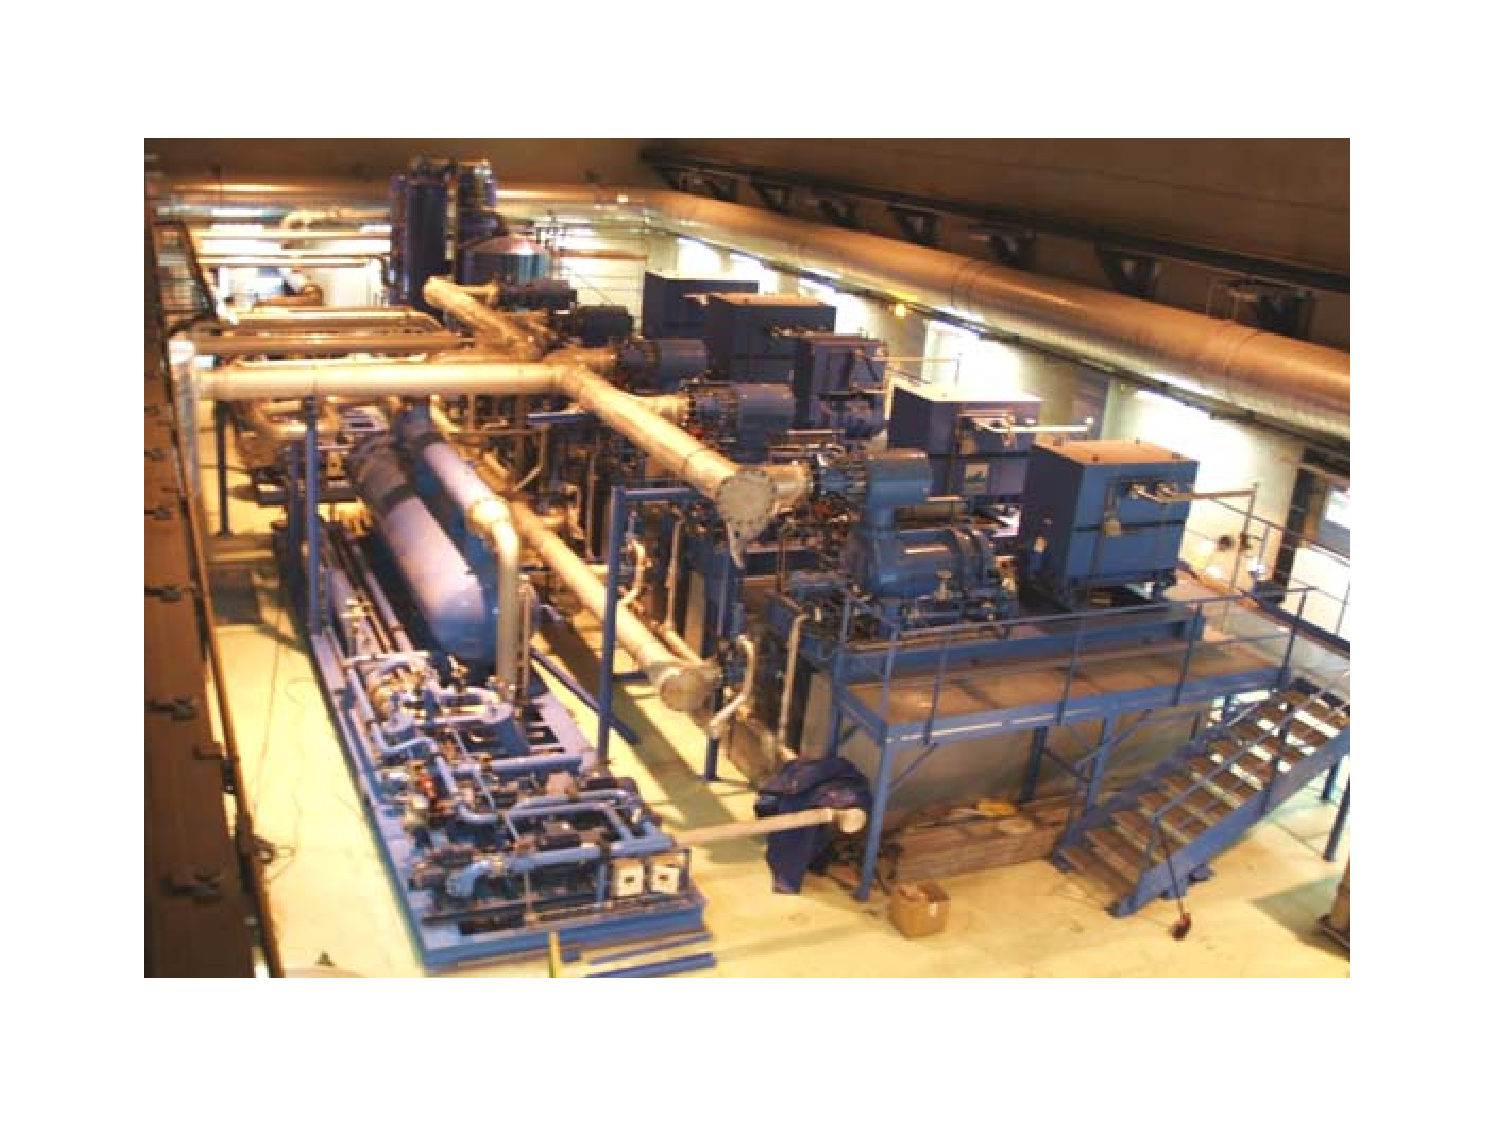
\includegraphics[width=\textwidth]{Figures/LHC_Diagrams/LHC_Cryogen_4p5KFridgeCompressor.pdf}
        \caption{The compressor station for the 4.5 K refrigeration system}\label{fig:lhc_cryo_4p5_compressor}
      \end{subfigure}
      ~ %add desired spacing between images, e. g. ~, \quad, \qquad, \hfill etc.
      % (or a blank line to force the subfigure onto a new line)
    \begin{subfigure}[h]{0.450\textwidth}
        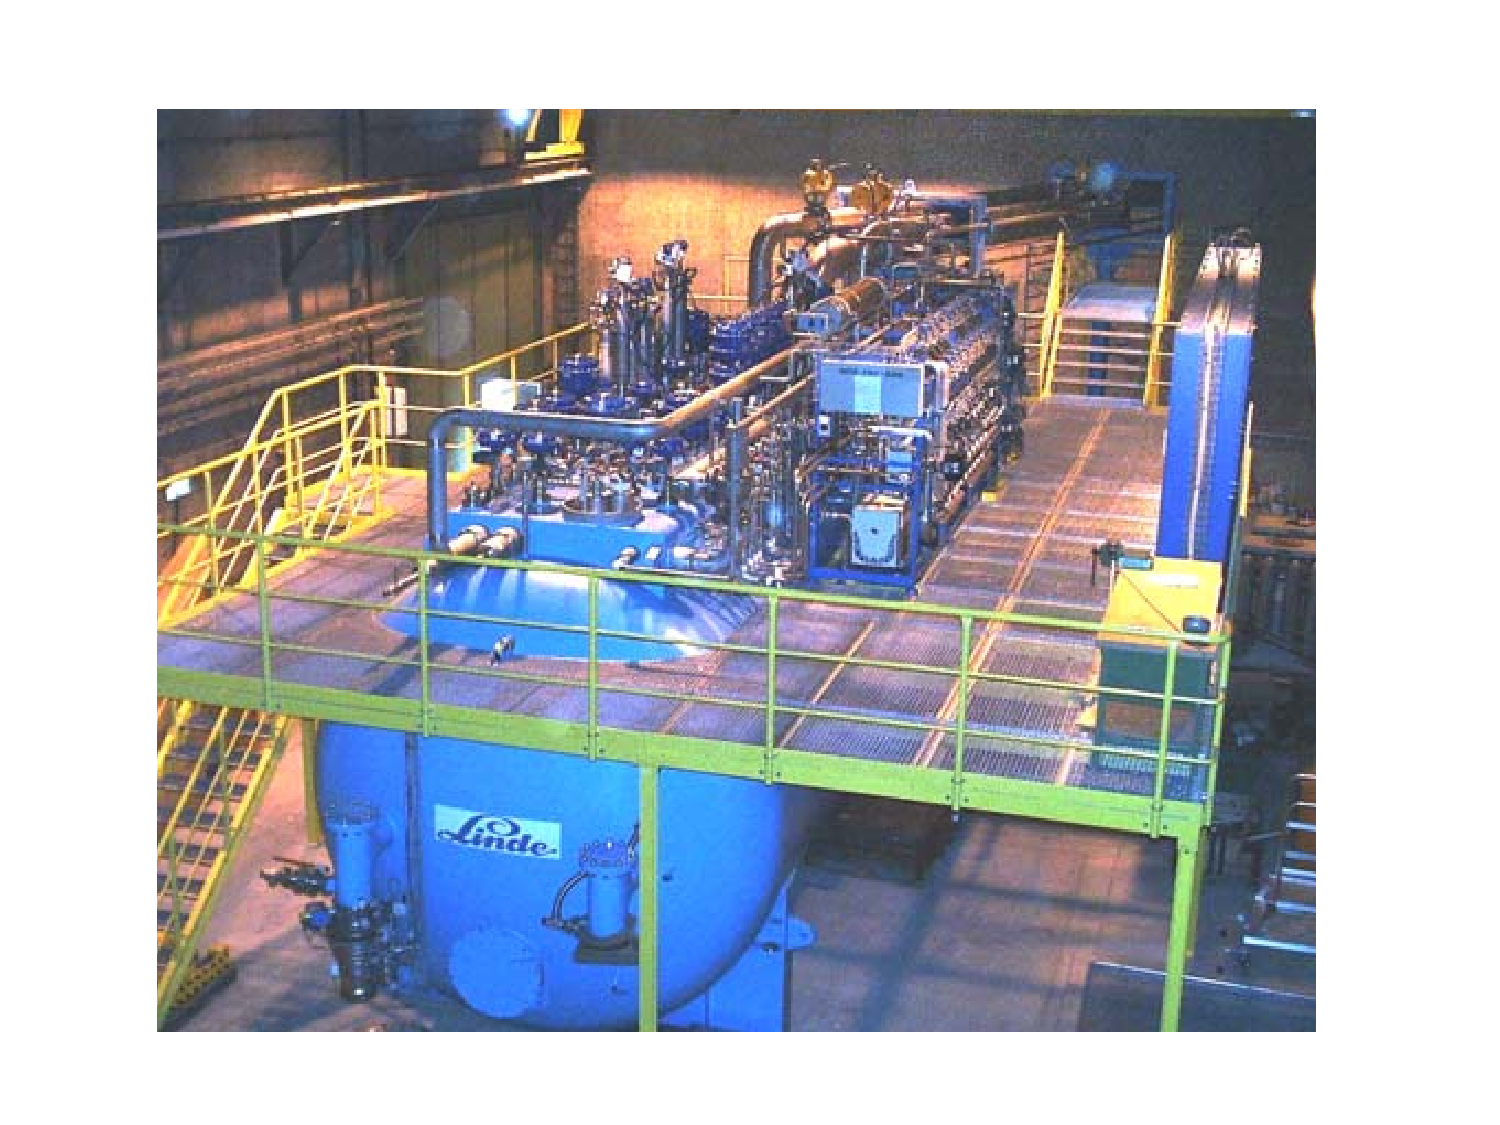
\includegraphics[width=\textwidth]{Figures/LHC_Diagrams/LHC_Cryogen4p5KFridge_Coldbox.pdf}
        \caption{The 4.5 K refrigeration system cold box, containing
          heat exchanging fins and turbines to cool the He}\label{fig:lhc_cryo_4p5_coldbox}
      \end{subfigure}
      \caption{Features of the 4.5 K refrigeration system \cite{LHC:LHC_cryogenicHe_system_Lebrun}}\label{fig:lhc_cryo_4p5}
\end{figure}

\par At each cryogenic plant, He is cooled to 80 K by circulating it
through refrigeration equipment with liquid nitrogen in the heat
exchangers\cite{LHC:LHC_lhc_cryogen_cernWebsite}.  Next, the He is
brought to 4.5 K with refrigerators recovered from the LEP experiment
\cite{LHC:LHC_cool_challenge}.  The He gas is first compressed and allowed
to expand, where it is cooled by losing energy through mechanical
turbo-expanders that run at up to 140,000 rpm on helium-gas
bearings, as shown in figure
\ref{fig:lhc_cryo_4p5}(\subref{fig:lhc_cryo_4p5_compressor}).  The He
is then liquified after passing through a vacuum sealed box containing
heat exchangers and more turbo-expanders
\cite{LHC:LHC_cryogenicHe_system_Lebrun}. The compressor for this
system is pictured in figure
\ref{fig:lhc_cryo_4p5}(\subref{fig:lhc_cryo_4p5_coldbox}).  Finally,
the liquified He is brought to 1.8 K with a refrigeration unit that
uses a cold compression train to decrease the saturation pressure, and
thus temperature as well. 

\begin{figure}[h]
   \centering
  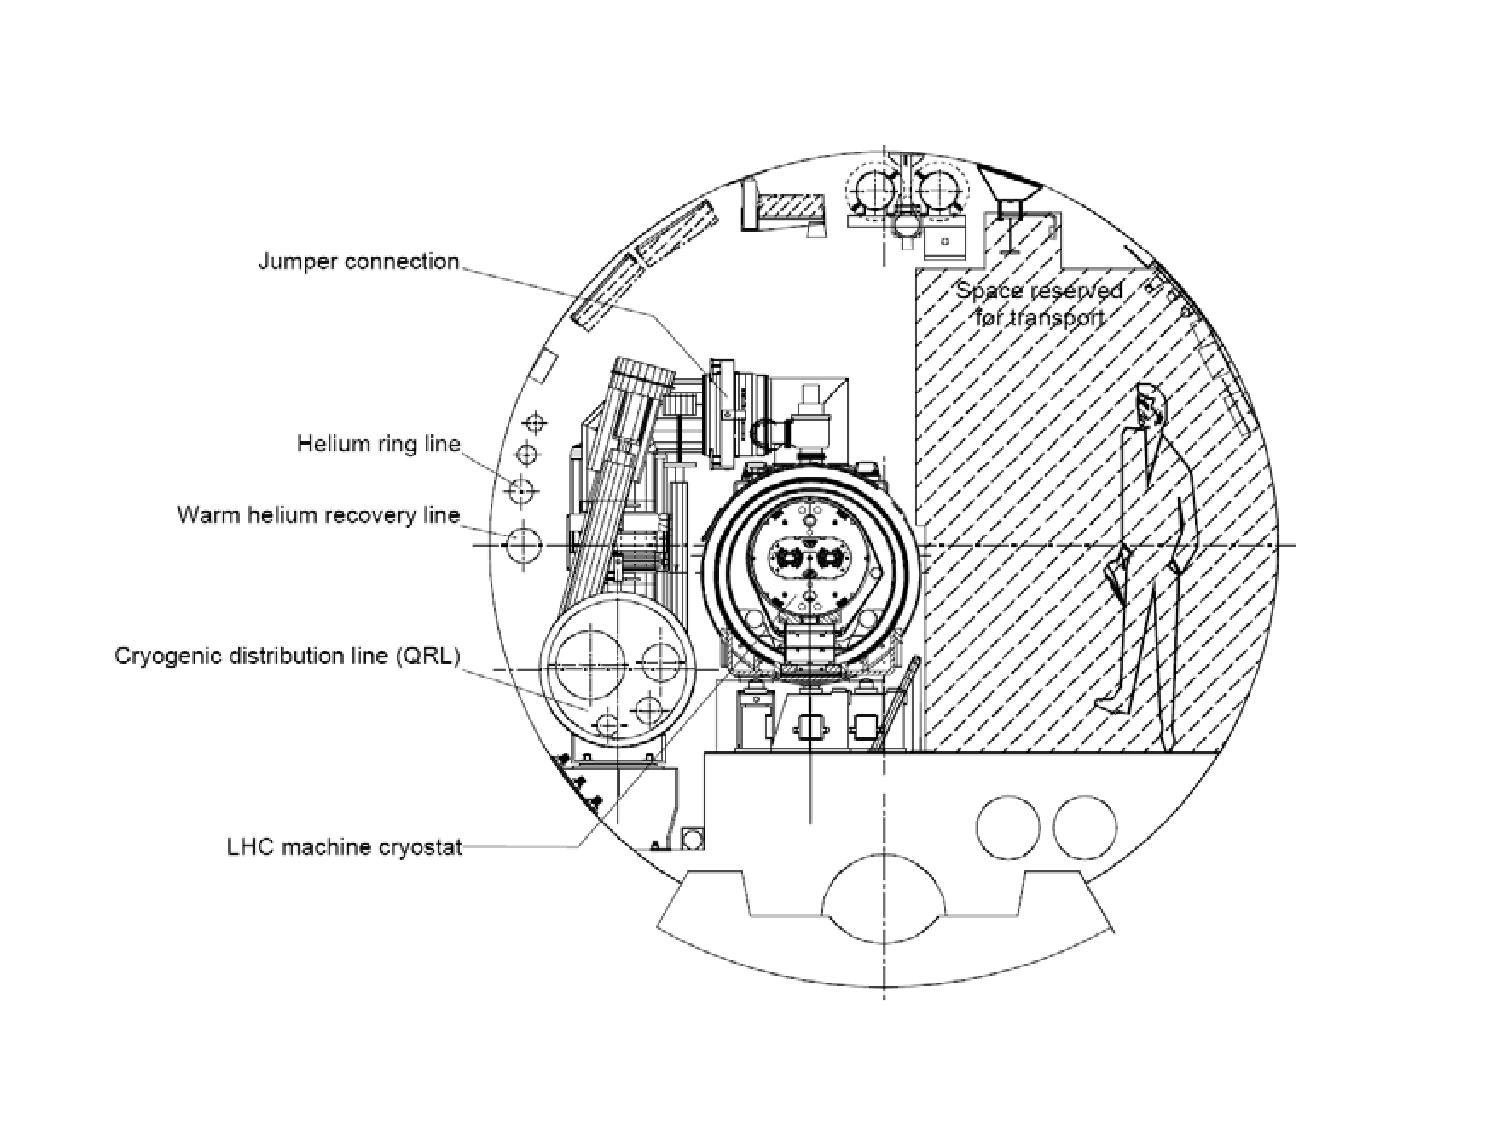
\includegraphics[width=0.6\textwidth]{Figures/LHC_Diagrams/LHC_CryogenInTunnel.pdf}
  \caption{Cross section schematic of the cryogenic distribution
    system in the LHC tunnel \cite{lhc:machine_description}} \label{fig:lhc_cryogen_tunnel_xs}
\end{figure}

\par In the LHC tunnel, a cryogenic distribution line runs parallel to
the machine \cite{LHC:LHC_cool_challenge}.  It consists of eight 3.2
km long cryostats, that contain the equipment to supply and recover
helium with temperatures ranging from 4 K to 75 K.  A total of 310
service modules, are used to control the system and provide safety
mechanisms against pressure buildup and magnet quenching.  Figure
\ref{fig:lhc_cryogen_tunnel_xs} shows a cross section of the cryogen
distribution system in the tunnel. 

\section{The LHC Vacuum System}
\label{lhc_vacuum_overview}

\par The LHC is also the largest operational vacuum system in the
world and is capable of achieving pressures lower than outer space
\cite{LHC:LHC_lhc_vacuum_cernWebsite}.  Three different types of
vacuum systems are used: one for insulating the helium distribution
lines, another for insulating the dipole magnets, and a final
ultra-high vacuum system for the beam pipe
\cite{lhc:machine_description}.  

\par The vacuum systems for insulating the helium distribution and
dipoles involves some 104 km of piping an over 250,000 welding
joints \cite{LHC:LHC_lhc_vacuum_cernWebsite}.  Pressure here is
required to be kept at $10^{-1}$ mbar, but at cryogenic temperatures,
pressures tend to equalize at a much lower level, to $10^{-6}$ mbar
($\sim10^{-9}$ atm) \cite{lhc:machine_description}.   

\begin{figure}[h]
   \centering
  \includegraphics[width=0.6\textwidth]{Figures/LHC_Diagrams/LHC_BeamScreen.jpg}
  \caption{Beam screen for the LHC, with slits to allow for easy
    pumping of residual gas molecules in the beam-pipe \cite{LHC:LHC_lhc_beamScreen_image}.} \label{fig:lhc_beam_screen}
\end{figure}

\par The most stringent requirements come on the vacuum of the
beam-pipe.  The beam must minimize the number of interactions it has
with any particles outside of the interaction region.  A pressure of
$10^{-10}$ to $10^{-11}$ mbar are maintained in the 54 km of
beam-pipe \cite{LHC:LHC_lhc_vacuum_cernWebsite}.  Weeks of cryogenic
pumping, eventually condenses gas trapped in the beam-pipe into a
liquid that can be absorbed by the walls of the beam-pipe.  The inside
beam-pipe is also coated with a thin layer of a special substance 
developed at CERN, a titanium-zirconium-vanadium alloy, which absorbs
residual particles when heated.  780 ion pumps are used to remove the
noble gases and methane, which do not interact with the substance,
which acts as its own distributed pumping system.  Room-temperature
sections of the beam-pipe are also heated to 300$^{\deg}$ to be
baked-out from the outside.  This is done to periodically remove 
any material which may have settled and become trapped. Additionally,
the beam-pipe is designed with a racetrack shape, which optimizes the
available aperture while leaving space for the cooling tubes, as shown
in figure \ref{fig:lhc_beam_screen}.  Slits also allow for gas
molecules to be easily pumped out from inside its volume.   

